% August 2017 (TOC contents linked in blue in pdf file)
%This template was prepared by Dorothea F. Brosius of the
%Institute for Electronics and Applied Physics, University of Maryland, College Park, MD
%The template was last updated in August 2017
%Thesis Main Page used with thesis.sty based on the
%University of Maryland Electronic Thesis and Dissertation (ETD) Style Guide (2016)

%The YourInformation file was created by Freja Nordsiek, 2014.
%Code for linking the TOC titles to the text in the pdf file was created by Freja Nordsiek, 2014.

% Select the version that fits how you are making this LaTeX document (its driver).
% The first two are the most likely ones to be needed.

 \newcommand{\mydriver}{pdflatex} %Making a PDF directly using pdflatex.
%\newcommand{\mydriver}{dvipdfmx} %Making a DVI and converting that to PDF using dvipdfmx.
%\newcommand{\mydriver}{dvipdfm} %Making a DVI and converting that to PDF using dvipdfm.
%\newcommand{\mydriver}{dvips} %Making a DVI and converting that to PS using dvips (may later be converted to PDF).
%\newcommand{\mydriver}{dvipsone} %Making a DVI and converting that to PS using dvipsone (may later be converted to PDF).
%\newcommand{\mydriver}{ps2pdf} %Same as the one for dvips except it is compatible with Ghostscript's PDF writer.


\documentclass[12pt,\mydriver]{thesis}  %12pt is larger than 11pt

\usepackage{titlesec}
   \titleformat{\chapter}
      {\normalfont\large}{Chapter \thechapter:}{1em}{}
\usepackage{graphicx}
\usepackage{cite}
\usepackage{lscape}
\usepackage{indentfirst}
\usepackage{latexsym}
\usepackage{multirow}
\usepackage{epstopdf}
\usepackage{tabls}
\usepackage{wrapfig}
\usepackage{slashbox}
\usepackage{longtable}
\usepackage{supertabular}
\usepackage{subeqn}
\usepackage{subfigure}

%hyperref
\usepackage[colorlinks=true,urlcolor=black,linkcolor=blue,citecolor=blue]{hyperref}

\newcommand{\tbsp}{\rule{0pt}{18pt}} %used to get a vertical distance after \hline
\renewcommand{\baselinestretch}{2}
\setlength{\textwidth}{5.9in}
\setlength{\textheight}{9in}
\setlength{\topmargin}{-.50in}
%\setlength{\topmargin}{0in}    %use this setting if the printer makes the the top margin 1/2 inch instead of 1 inch
\setlength{\oddsidemargin}{.55in}
\setlength{\parindent}{.4in}
\pagestyle{empty}

% Pete's editing special sauce
% \usepackage[usenames,dvipsnames,svgnames,table]{xcolor}
\newcommand{\todo}[1]{{\textcolor{red}{#1}}}
\newcommand{\pjk}[1]{{\textcolor{red}{PJK: #1}}}
\newcommand{\ben}[1]{{\textcolor{orange}{Ben: #1}}}

\begin{document}
\pagestyle{empty}
%Abstract Page

\hbox{\ }

\renewcommand{\baselinestretch}{1}
\small \normalsize

\begin{center}
\large{{ABSTRACT}}

\vspace{3em}

\end{center}
\hspace{-.15in}
\begin{tabular}{ll}
Title of dissertation:    & {\large  PLANETARY SCALE DATA STORAGE }\\
\ \\
&                          {\large  Benjamin Bengfort} \\
&                           {\large Doctor of Philosophy, 2018} \\
\ \\
Dissertation directed by: & {\large  Professor Peter J. Keleher} \\
&               {\large  Department of Computer Science } \\
\end{tabular}

\vspace{3em}

\renewcommand{\baselinestretch}{2}
\large \normalsize

The success of virtualization and container-based application deployment has fundamentally changed computing infrastructure from dedicated hardware provisioning to on-demand, shared clouds of computational resources. One of the most interesting effects of this shift is the opportunity to localize applications in multiple geographies and support mobile users around the globe. With relatively few steps, an application and its data systems can be deployed and scaled across continents and oceans, leveraging the existing data centers of much larger cloud providers.

The novelty and ease of a global computing context means that we are closer to the advent of an Oceanstore, an Internet-like revolution in personalized, persistent data that securely travels with its users. At a global scale, however, data systems suffer from physical limitations that significantly impact its consistency and performance. Even with modern telecommunications technology, the latency in communication from Brazil to Japan results in noticeable synchronization delays that violate user expectations. Moreover, the required scale of such systems means that failure is routine.

To address these issues, we explore consistency in the implementation of distributed logs, key/value databases and file systems that are replicated across wide areas. At the core of our system is hierarchical consensus, a geographically-distributed consensus algorithm that provides strong consistency, fault tolerance, durability, and adaptability to varying user access patterns. Using hierarchical consensus as a backbone, we further extend our system from data centers to edge regions using federated consistency, an adaptive consistency model that gives satellite replicas high availability at a stronger global consistency than existing weak consistency models.

In a deployment of 105 replicas in 15 geographic regions across 5 continents, we show that our implementation provides high throughput, strong consistency, and resiliency in the face of failure. From our experimental validation, we conclude that planetary-scale data storage systems can be implemented algorithmically without sacrificing consistency or performance.
 %(must be first, required, non-numbered)
%Titlepage

\thispagestyle{empty}
\hbox{\ }
\vspace{1in}
\renewcommand{\baselinestretch}{1}
\small\normalsize
\begin{center}

\large{{GOAL TRAJECTORIES DURING INTERACTIVE-KNOWLEDGE GOAL REASONING}}\\
\ \\
\ \\
\large{by} \\
\ \\
\large{Benjamin Bengfort}%Your full name as it appears in University records.
\ \\
\ \\
\ \\
\ \\
\normalsize
Dissertation submitted to the Faculty of the Graduate School of the \\
University of Maryland, College Park in partial fulfillment \\
of the requirements for the degree of \\
Doctor of Philosophy \\
2016
\end{center}

\vspace{7.5em}

\noindent Advisory Committee: \\
Professor Don Perlis, Chair/Advisor \\
Dr. Michael Cox, Co-Advisor \\
Professor James A. Reggia \\
Professor Ben Shneiderman \\
Dr. David Aha
 %(must follow Abstract, required, non-numbered)
%Copyright

\thispagestyle{empty}
\hbox{\ }

\vfill
\renewcommand{\baselinestretch}{1}
\small\normalsize

\vspace{-.65in}

\begin{center}
\large{\copyright \hbox{ }Copyright by\\
Benjamin Bengfort  %Type your name as it appears in University records
\\
2016}
\end{center}

\vfill
 %(highly recommended, non-numbered)

%Pages from this point start at lower-case Roman number ii)
\pagestyle{plain} \pagenumbering{roman} \setcounter{page}{2}
% \addcontentsline{toc}{chapter}{Preface}
% %Preface
\pagestyle{plain}\pagenumbering{roman} \setcounter{page}{2}
\renewcommand{\baselinestretch}{2}
\small\normalsize
\hbox{\ }

\vspace{-.65in}

\begin{center}
\large{Preface}
\end{center}


If needed.
  %(if present, start at lower-case Roman number ii)
% \addcontentsline{toc}{chapter}{Foreword}
% %Foreword

\renewcommand{\baselinestretch}{2}
\small\normalsize
\hbox{\ }
 
\vspace{-.65in}

\begin{center}
\large{Foreword} 
\end{center} 

If needed.
 %(if present, lower-case Roman)
\addcontentsline{toc}{chapter}{Dedication}
%Dedication

\renewcommand{\baselinestretch}{2}
\small\normalsize
\hbox{\ }

\vspace{-.65in}

\begin{center}
\large{Dedication}
\end{center}

This dissertation is dedicated to my grandmothers, both of whom overcame extreme hardship so that their children and grandchildren could attain the highest levels of education.
 %(if present, lower-case Roman)
\addcontentsline{toc}{chapter}{Acknowledgements}
%Acknowledgments

\renewcommand{\baselinestretch}{2}
\small\normalsize
\hbox{\ }

\vspace{-.65in}

\begin{center}
\large{Acknowledgments}
\end{center}

\vspace{1ex}

I could not have done this alone. 
 %(if present, lower-case Roman)

\renewcommand{\baselinestretch}{1}
\small\normalsize
\tableofcontents %(required, lower-case Roman)
\newpage
\listoftables %(if present, lower-case Roman)
\newpage
\listoffigures %(if present, lower-case Roman)
\newpage
% LIST OF ABBREVIATIONS
\addcontentsline{toc}{chapter}{List of Abbreviations}
%List of Abbreviations


\renewcommand{\baselinestretch}{1}
\small\normalsize
\hbox{\ }

\vspace{-4em}

\begin{center}
\large{List of Abbreviations}
\end{center}

\vspace{3pt}

\begin{supertabular}{ll}
EC & Eventual consistency \\
HC & Hierarchical consensus \\
%$\alpha$ & alpha \\
%$\beta$  & beta \\
%&  \\
%IREAP & Institute for Research in Electronics and Applied Physics \\
%NSA & National Security Agency
\end{supertabular}


\newpage
\setlength{\parskip}{0em}
\renewcommand{\baselinestretch}{2}
\small\normalsize

%Pages from this point start at Arabic numeral 1
\setcounter{page}{1}
\pagenumbering{arabic}
%Chapter 1

\renewcommand{\thechapter}{1}

\chapter{Introduction}
% Going for about 5 pages or so here.

Ubiquitous computing is becoming the norm.
    More users are mobile
    Non-human users (IoT is generating a lot of data)
    Applications are global
    Requires transparent persistence

Oceanstore provides a model for untrusted global-scale data
    Requires connectivity, security, durability (consistency), divorced from location
    Oceanstore model relies on encryption and async commit with conflict resolution
    Two tiers for updates: Byzantine quorum and eventual consistency layer

Cloud revolution
    The model has changed: client-server interactions and siloed data (not files)
    Trusted replicas are available across the globe (or secured with encryption/SUNDR)
    Updates are still too fast, however, centralization means that consistency is now the number one issue.
    FIGURE: locations of cloud computing data centers

Toward Edge and Fog computing
    Data systems are becoming increasingly complex (many publishers, few subscribers, distributed accesses)
    Sensor networks, energy platforms, self-driving vehicle networks
    Greater localization is required

Our vision: planetary-scale data storage
    First tier: strong, resilient, fast consensus with hierarchical consensus
    Second tier: highly available eventual consistency federated with strong consistency
    Adaptiveness: online monitoring and network adaptation

Contributions:
    Design, implementation, and evaluation of hierarchical consensus
    Design, implementation, and evaluation of federated consistency
    Design, implementation, and evaluation of bandit-based anti-entropy
    Design and implementation of planetary-scale key/value store
    Design and implementation of a planetary-scale file system
    Description and discussion of distributed systems in the very wide area
    Description and discussion of dependent scaling of consensus algorithms

Organization of the rest of the paper

%Chapter 2

\renewcommand{\thechapter}{2}

\chapter{A Geo-Distributed System Architecture}
\label{ch:architecture}

% Goals for this chapter:
%   1. Present a case that geo-replicated systems are more common
%   2. Present the challenges for a geo-replicated system
%   3. Outline our proposed architecture
%   4. Outline our proposed apps: distributed log, kv store, file system

% At the end of this chapter the reader should believe that planetary-scale  data systems are necessary and that existing solutions don't meet current requirements exactly.

% The primary purpose of this chapter is to show that our core component, hierarchical consensus is the center of any geo-replicated system.

The advent of cloud computing has accelerated both commercial and academic interest in distributed systems connected via wide area networks and the Internet.
Cloud computing exists because large Internet companies, which had deployed extremely large data centers around the world to meet global user demand for their services, created extra capacity that could be leased to tenants on-demand.
The global nature of cloud providers means that there is an opportunity for more common usage of geographically replicated data systems besides the specialized systems they developed for internal use.
Though these systems have been made available to customers as provisioned services, they suffer from application-specific data models to narrow to solve general problems.

The specialization of the current generation of distributed systems is designed to optimize their behavior when deployed within a pristine data center context.
This environment, with strong facility support and backbone communications, allows design choices that optimistically assume that repairs will be made quickly and that redundancy need only protect from few failures at a time~\cite{bermbach_eventual_2011,wada_data_2011,node_failure,jhawar_fault_2013}.
This has led to a general architecture for geo-replication that provisions consistency requirements across transactions, individual objects, and within blocks stored on disk, often leading to multiple, independent consistency models within the same system.
This design leads to confusion about where data is stored and what guarantees can be made about each access.

Instead, a single, global consistency model is required to correctly reason about a single, global system's behavior.
The central thesis of this dissertation is that this can only be achieved with a globally-distributed consensus protocol.

Consistency depends on the network environment and in highly curated data centers, systems are built using localized consensus~\cite{bolosky_paxos_2011}.
Outside the data center, however, single process failures show the impossibility of distributed consensus~\cite{fischer_impossibility_1985}.
Therefore our approach is a continuous, flexible consistency model with geographic consensus at its core and a federated approach at its edge.
The result is a single, understandable consistency model that leads to an architecture capable of supporting global systems both inside and outside of the data center.

In this chapter, we will describe the details of our proposed architecture for a planet-wide distributed data store.
To motivate our architectural decisions, we first describe the motivations and challenges for the design of such a system.
We motivate our work in two parts.
First, we argue that there is a new software deployment paradigm that requires geographic replication.
Second, we argue that existing geo-replicated data stores are not general enough to meet the needs of that paradigm.
We follow these motivations with the challenges of geo-replication described as requirements, which we will then use to present an overview of our system architecture.

\section{Challenges and Motivations}
\label{ch02_challenges_and_motivations}

Many of the world's most influential companies grew from the ashes of the dot-com bubble of the 1990s, which paid for an infrastructure of fiber-optic cables, giant server farms, and research into mobile wireless networks~\cite{casey_blockchain_2018}.
As these companies filled market voids in eCommerce, search, and social networking, they created new database technologies to leverage the potential of underused computational resources and low latency/high bandwidth networks that connected them, eschewing more mature systems that were developed with resource scarcity in mind~\cite{stonebraker_what_2005,stonebraker_mapreduce_2010}.
What followed was the rise and fall of NoSQL data systems, a microcosm of the proceeding era of database research and development~\cite{mohan_history_2013}.

Although there are many facets to the story of NoSQL, what concerns us most is the use of NoSQL to create geographically distributed systems, as these systems paved the way to the large-scale storage systems in use today.
The commercial and open source interest in geo-replicated systems both for big data analysis and Web application development has led to the development of many database and file systems.
These systems share common traits, allowing us to describe a general architecture for distributed systems.
More importantly, the prevalence of such systems has led to a new application development paradigm: modern software must be designed as a global services.

\subsection{A New Application Development Paradigm}
\label{ch02_new_software_paradigm}

The launch of the augmented reality game Pokémon GO in the United States was an unmitigated disaster~\cite{kain_pokemon_2016}.
Due to extremely overloaded servers from the release's extreme popularity, users could not download the game, login, create avatars, or find augmented reality artifacts in their locales.
The company behind the platform, Niantic, scrambled quickly, diverting engineering resources away from their feature roadmap toward improving infrastructure reliability.
The game world was hosted by a suite of Google Cloud services, primarily backed by the Cloud Datastore~\cite{cloud_datastore}, a geographically distributed NoSQL database.
Scaling the application to millions of users therefore involved provisioning extra capacity to the database by increasing the number of shards as well as improving load balancing and autoscaling of application logic run in Kubernetes~\cite{Kubernetes} containers.

Niantic's quick recovery is often hailed as a success story for cloud services and has provided a model for elastic, on demand expansion of computational resources.
A deeper examination, however, shows that Google's global high speed network was at the heart of ensuring that service stayed stable as it expanded ~\cite{stone_bringing_2016}, and that the same network made it possible for the game to immediately become available to audiences around the world.
The original launch of the game was in 5 countries -- Australia, New Zealand, the United States, the United Kingdom, and Germany.
The success of the game meant worldwide demand, and it was subsequently expanded to over 200 countries starting with Japan~\cite{yamazaki_developer_2016}.
Unlike previous games that were restricted with region locks~\cite{region_locking}, Pokémon GO was a truly international phenomenon and Niantic was determined to allow international interactions in the game's feature set, interaction which relies on Google's unified international architecture and globally distributed databases.

Stories such Niantic's deployment are increasingly becoming common and medium to large applications now \emph{require developers to quickly reason about how data is distributed in the wide area, different political regions, and replicated for use around the world}.

It is not difficult to find many examples of companies and applications, from large to small, that have international audiences and global deployments which highlight the new challenges of software development.
Dropbox has users in over 180 countries and is supported in 20 languages, maintaining offices in 12 locations from Herzliya to Sydney \cite{dropbox}.
Slack serves 9 million weekly active users around the world and has 8 offices around the world, prioritizing North America, Europe, and Pacific regions \cite{slack}.
WeWork provides co-working space in 250+ international applications and uses an app to manage global access and membership \cite{wework_global_access}.
Tile has sold 15 million of its RFID trackers worldwide and locates 3 million unique items a day in 230 countries \cite{tile}.
Trello, a project management tool, has been translated into 20 languages and has 250 million world-wide users in every country except Tuvalu; their international rollout focused on marketing and localization \cite{trello}.
Runkeeper~\cite{runkeeper} and DarkSky~\cite{darksky} are iOS and Android apps that have millions of global users and struggled to make their services available in other countries, but benefitted from international app stores.
Signal and Telegraph, both encrypted messaging apps, have grown primarily in countries at the top of Transparency International's Corruption Perception Index~\cite{signal}.

The new application development paradigm, even for small applications, is to build with the thought that your application will soon be scaling across the globe.
None of the applications described above necessarily have geography-based requirements in the same way that an augmented reality or airline reservations application might, just a large number of users who regularly use the app from a variety of geographic locations.
Web developers are increasingly discussing and using container based approaches both for development and small-scale production.
Web frameworks have built in localization tools that are employed by default.
Services are deployed on autoscaling cloud platforms from the start.

To address this paradigm shift, cloud service providers have expanded their offerings to include use of their distributed data stores to application developers, as in the case of Niantic.
This presents two problems, however.
First, those systems were designed for the huge applications of the Internet companies themselves, not for the general needs of a large audience of developers.
Second, cloud providers organized their services around geographically distinct regions, allowing their tenants the choice to deploy their applications in one or more regions.
As a result, tenants naturally choose cloud regions based on the locations of their users and treat regions as independent deployments from both a software and billing perspective.
Even though there may be some cross-region backup to prevent catastrophic failures, region-specificity usually means that services are deployed piecemeal and partitioned.

Region-based organization of cloud services has ensured that users are able to minimize latencies and provide applications to areas of interest, but applications have increasingly become more global.
The possibility of region-agnostic deployment is tantalizing, particularly as larger applications spend a non-trivial amount of administration time determining where writes to objects are going to optimize their systems.
Consistent updates across regions are not even considered as a possibility because in-house cloud services used data models that avoided large latencies wherever possible.
Moreover, as we will see in the next section, the design of provisioned cloud databases have made it difficult to reason about consistent behavior.
Not only is there a need for strong consistency semantics, data-location awareness, and geo-replication in distributed data storage systems, there is also the need for a familiar and standardized storage API.

\subsection{Building Geo-Replicated Services}
\label{ch02_systems_background}

The growth of database systems distributed across the wide-area started with large Internet companies like Yahoo~\cite{pnuts}, Google~\cite{bigtable}, and Amazon~\cite{dynamo} but quickly led to academic investigations.
One reason that the commercial systems enjoyed this academic attention was that at the time, the unique scale of their usage validated the motivation behind their architecture.
However their success has meant that these types of scales are no longer limited to huge software systems.
The development of geo-replicated services has therefore undergone several phase shifts, and has led to a general framework that underlies most current systems.

The first shift was the creation of highly available, sharded systems intended to meet the demand of increasing numbers of clients.
Commercially, these types of systems include Dynamo~\cite{dynamo} and BigTable~\cite{bigtable}, which in turn spawned open source and academic derivatives such as Cassandra~\cite{cassandra} and HBase~\cite{hbase}.
Although these systems did support many concurrent accesses, they achieved their availability by relaxing consistency, which many applications found to be intolerable.
The second shift was a return to stronger consistency, even at the cost of decreased performance or expensive engineering solutions.
Again, commercial systems led the way with Megastore~\cite{megastore} and Spanner~\cite{spanner} along with academic solutions such as MDCC~\cite{mdcc} and Calvin~\cite{calvindb,calvinfs}.
Part of this realignment was a reconsideration of the base assumptions that drove the NoSQL movement as expressed in the CAP theorem~\cite{cap,pushing_cap}.
The new thinking is that the lines between availability, partition tolerance, and consistency may not be as strictly drawn as previously theorized~\cite{hat,consistency_tradeoffs,cap_rules_change}.
This has led to a final shift, the return of SQL, as the lessons learned during the first two phases are applied to more traditional systems.
As before, both commercial systems, such as Aurora~\cite{aurora} and Azure SQL~\cite{azure_sql_database}, and open source systems such as Vitess~\cite{vitess} and CockroachDB~\cite{cockroachdb} are playing an important role in framing the conversation about consistency in this phase.

% This brief and limited description of the history of NoSQL distributed systems serves to set the tone for two primary points. First, designing distributed systems to support a large number of users across large geographies entails a number of challenges and trade-offs due to physical limitations that no single architecture has been able to fully cover. Second, there exists commercial and practical motivations to build such systems and these motivations have been the impulse toward academic research. With this backdrop in mind, we explore in this chapter the question of whether a planetary-scale data system is really necessary, and the challenges that we face when designing such systems.

These systems have defined several strategies from relaxed consistency to interval time that are essential to understanding geo-replicated services.
The first and primary strategy, however, is to shard data into independent groups of semi-related objects.
A shard can be specifically defined either as buckets of objects, tablets of contiguous rows, or in the most extreme cases, individual objects.

Sharding allow extremely massive databases and file systems to be broken down into smaller, related pieces that are more easily managed in a distributed context.
Sharding allows concurrent access to objects without synchronization.
If a shard is defined within a specific region, then it is easy to prioritize local accesses and coordination with that region.
Sharding also provides a data model for underlying redundant storage.
If a tablet can be written to a specific page on disk, that page can also be replicated to more easily colocate replicas with data.
If multiple shards need to be accessed simultaneously in a transaction, then
only the shards involved in the transaction need be coordinated, while all other shards can remain independent.

The unit of coordination is therefore at the shard level.
The namespace of the system must be allocated to individual components of the system, which must be globally available, and requires coordination to move part of the namespace from one region to another.
Accesses to data on disk for individual objects must also be allowed to happen in a fault-tolerant manner, which requires coordination between several replicas to guarantee no data loss.
Finally, transactions that require access to multiple objects must be coordinated to ensure atomic guarantees.
To support all of these features in a system, a multi-process architecture of independent components for geo-replication is generally deployed, as shown in Figure~\ref{fig:ch02_distributed_architecture}.

\begin{figure}
    \begin{center}
        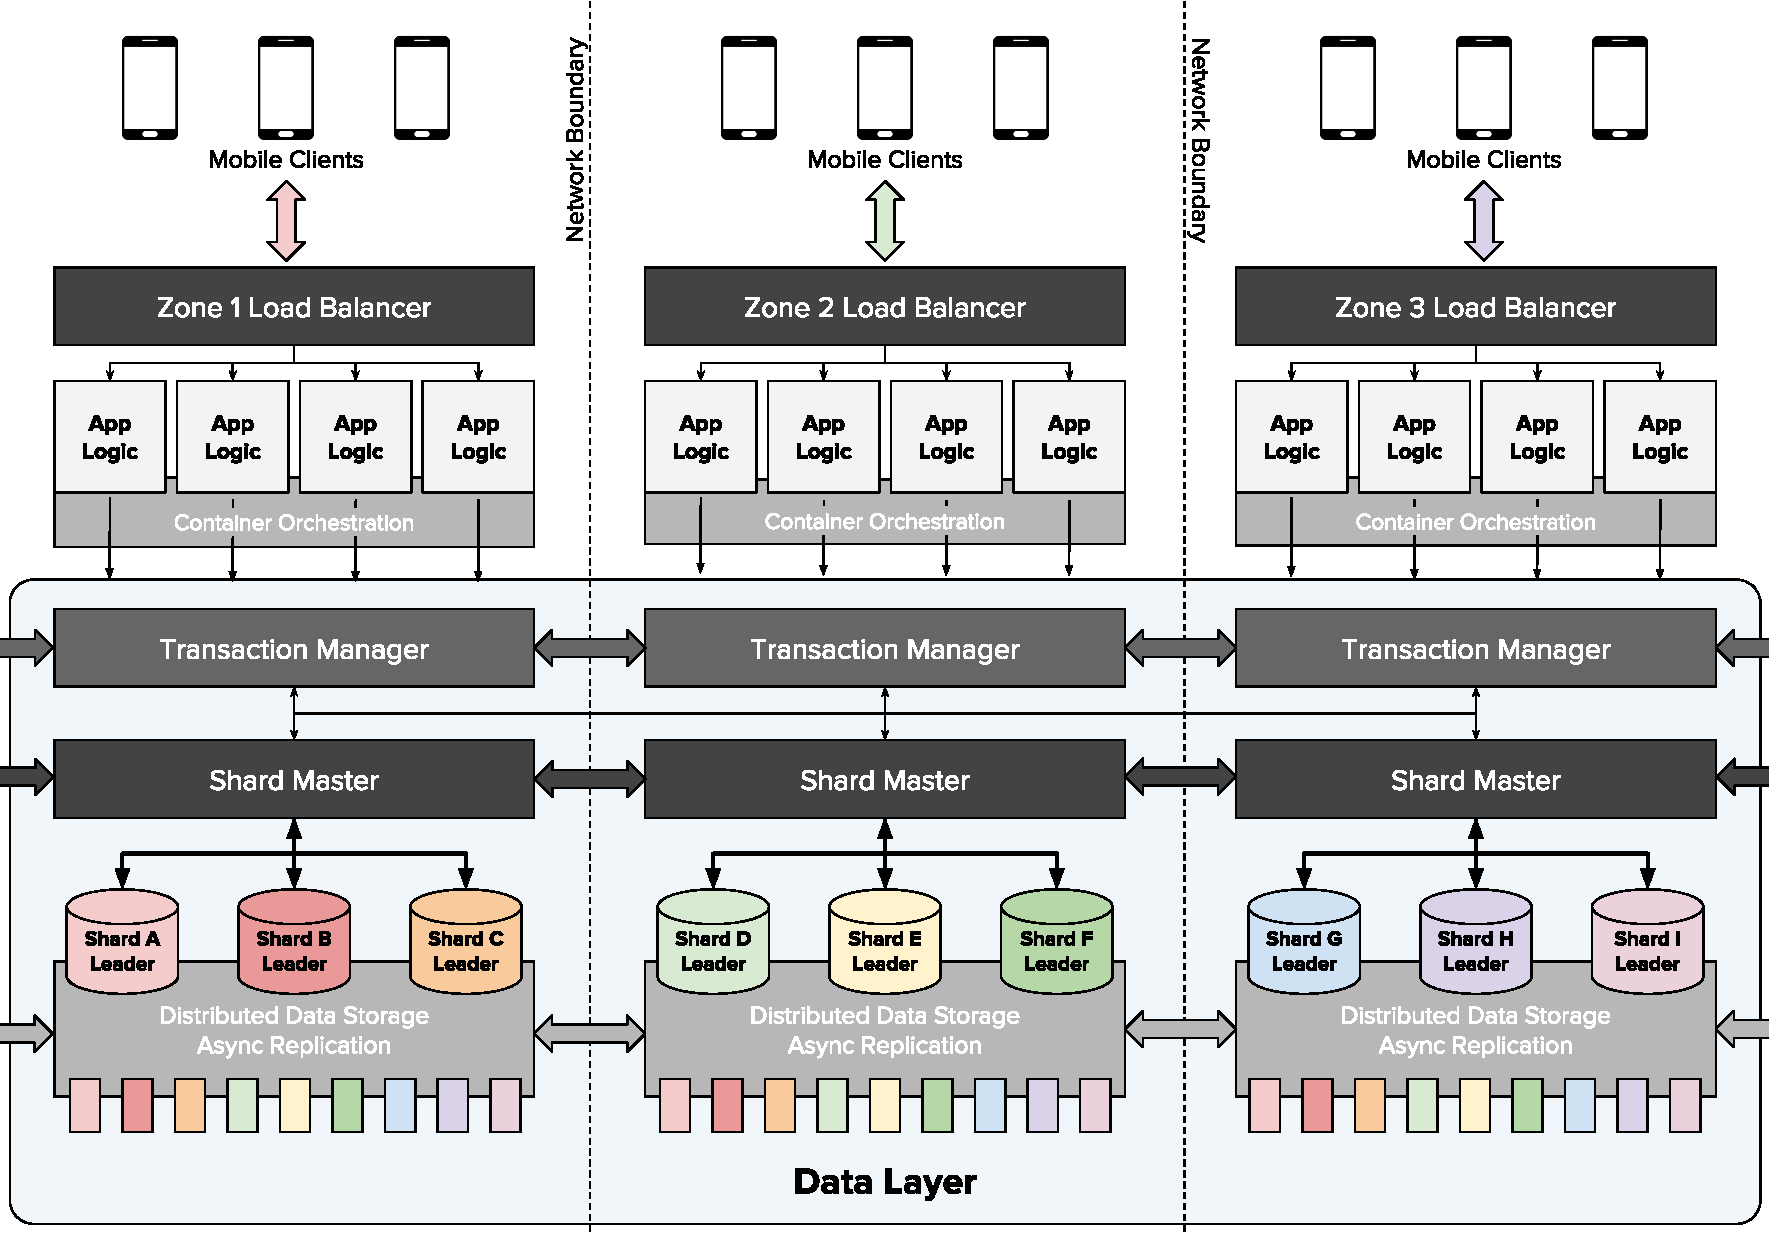
\includegraphics[width=5in]{figures/ch02_distributed_architecture.pdf}
    \end{center}
    \renewcommand{\baselinestretch}{1}
    \small\normalsize

    \begin{quote}
        \caption[A Generalized Geo-Distributed System Architecture]{A generalized architecture of a geographically distributed application using a basic sharding strategy. The namespace of the database is coordinated by shard masters, which point to quorums of replicas who replicate data over multiple disks. Accesses to multiple objects are coordinated via transaction managers.}
        \label{fig:ch02_distributed_architecture}
    \end{quote}
\end{figure}
\renewcommand{\baselinestretch}{2}
\small\normalsize

Clients access geographically-replicated data systems either by making geographic based requests via domain name (e.g. requesting a \texttt{.ca} addressed service vs. a \texttt{.fr} address) or by using IP and ping based network location~\cite{geoping}.
Multiple, concurrent requests are load-balanced to container based compute nodes that hold application logic, elastically scaled to meet changing demand~\cite{load_balancing}.
Though this aspect of distributed applications is outside the scope of a geo-replicated data store, the increased frequency of accesses across multiple regions increases the likelihood of collisions -- concurrent access by multiple clients to the same object(s), which leads to the consistency concerns of this dissertation.

The data layer follows the application logic layer and is the layer that must coordinate accesses from many simultaneous geographies.
If the data layer supports transactions~\cite{hat,calvindb,calvinfs,cockroachdb,vitess,aurora} then the top level of coordination is the transaction manager, which is responsible for identifying the shards that manage the objects and correctly committing or rolling back the transaction.
Other systems support snapshot isolation for read-transactions~\cite{spanner,megastore}, ensuring that all reads for a specified time window are consistent.

If the data layer does not support transactions or if only a single object is being accessed, then the system must coordinate with the shard master, a process that allocates the namespace to the replicas that manage those objects.
Some systems use the data-model directly, using key-space addressing to determine the locality of objects~\cite{bigtable,spanner}, others use consistent hashing~\cite{chord,scatter} to balance objects around a hash ring, coordinating the insertion and removal of name management servers.
However, if the preservation of data locale and the ability to move objects between regions is required, then a synchronized lookup table must be used.
The most popular mechanism to achieve namespace synchronization is to use a lock service such as Chubby~\cite{chubby} or etcd~\cite{etcd_raft} to hand out leases for which an replica is expected to manage accesses.

Once the replica that manages the shard is discovered, the actual access must occur.
There are several mechanisms for this that use quorums of replicas to make decisions.
Weak consistency models of access use overlapping read and write quorums of varying sizes along with eventual replication of the data~\cite{dynamo}.
Strong consistency models of access use Paxos~\cite{paxos} as the basis for high performance data storage~\cite{bolosky_paxos_2011,lampson_how_1996} -- consensus will be discussed in detail in the next section.
To further increase write throughput, accesses append commands to a distributed log that are applied asynchronously to the underlying data store, so long as the command is committed to the log, it is guaranteed to be written to storage~\cite{logbase,logfs,log_memory}.

Finally, data must be written to stable storage, usually on clusters of disks that are also distributed so as to prevent data loss in the likely event that a disk fails.
Many geo-replicated data systems also use a distributed file system for underlying storage.
BigTable stores its data on GFS~\cite{gfs}, f4~\cite{f4} on top of HDFS~\cite{hdfs}, an open source implementation of GFS, and Spanner stores its data on Colossus~\cite{colossus}, the next generation of GFS.
Other distributed databases such as BTrDB~\cite{btrdb} use the Ceph~\cite{ceph} file system for data replication and because of requirements for location-fault tolerance, it is becoming increasingly rare that hardware based schemes such as RAID~\cite{raid} are used to ensure data durability.

\begin{figure}
    \begin{center}
        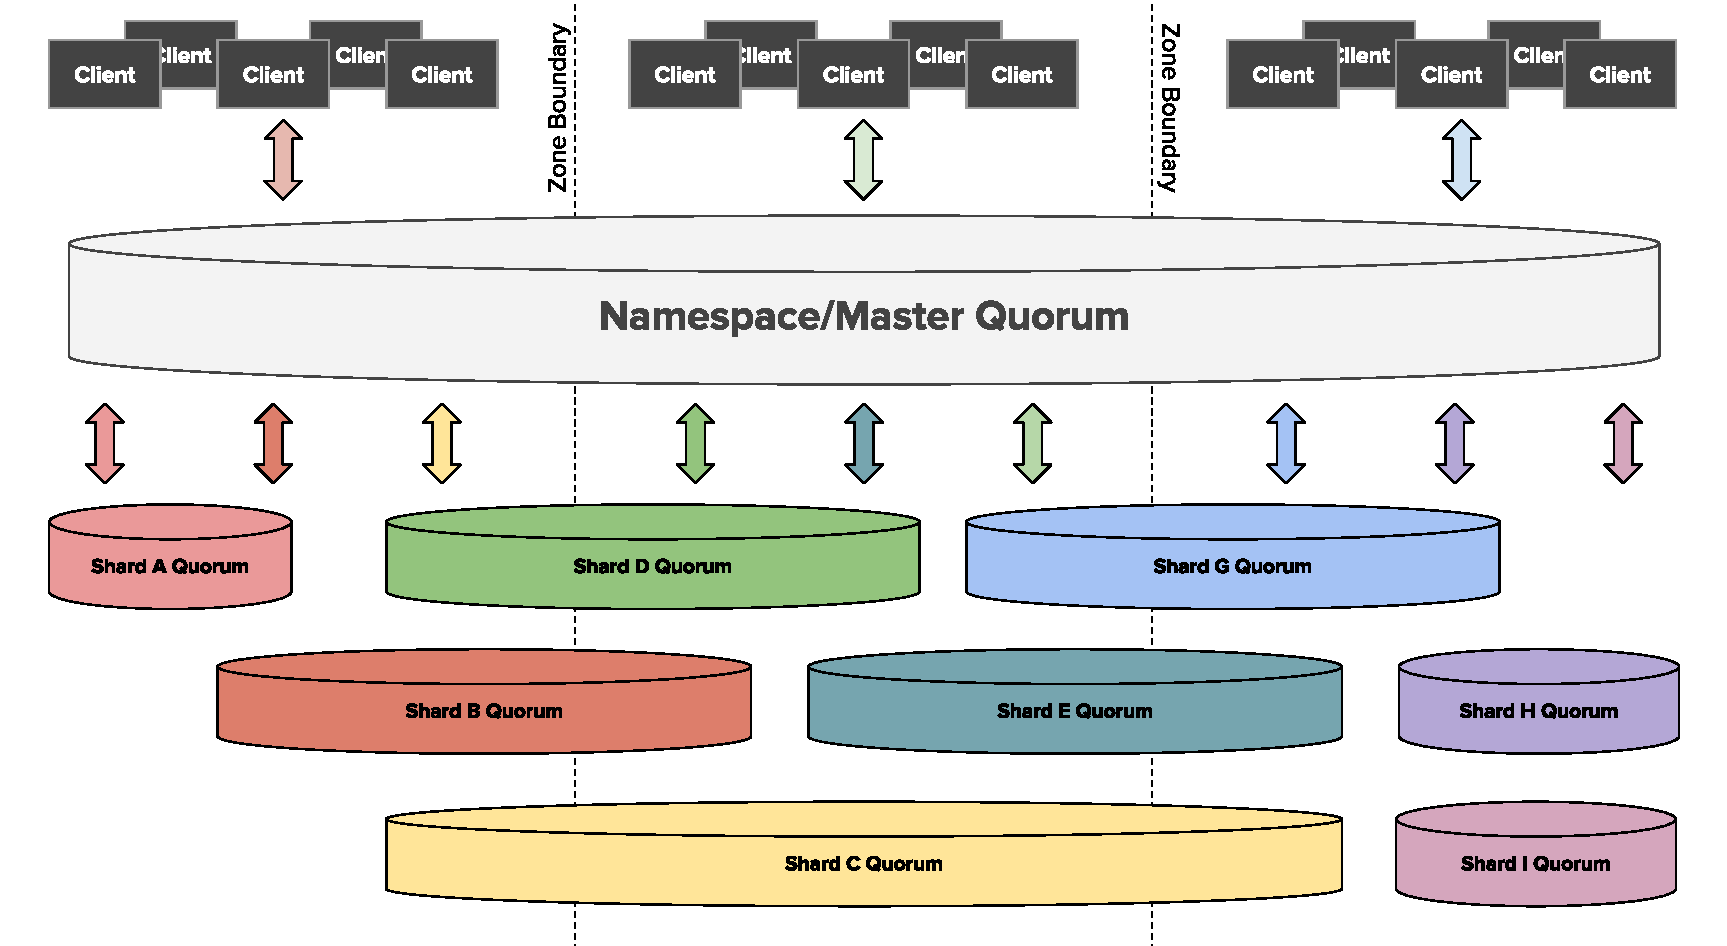
\includegraphics[width=5in]{figures/ch02_simplified_distributed_consensus_alt.pdf}
    \end{center}
    \renewcommand{\baselinestretch}{1}
    \small\normalsize

    \begin{quote}
        \caption[A Simplified Geo-Distributed Consensus Blueprint]{Figure~\ref{fig:ch02_distributed_architecture} can be simplified to a single consensus architecture with a top-level consensus quorum making namespace decisions and directing requests to per-object quorums that are replicated within a single data center or across regions or zones.}
        \label{fig:ch02_simplified_distributed_consensus}
    \end{quote}
\end{figure}
\renewcommand{\baselinestretch}{2}
\small\normalsize

The description above and Figure~\ref{fig:ch02_distributed_architecture} are a useful blueprint for designing large scale geo-replicated systems and generalizes many of the themes and attributes of a wide variety of systems.
The problem with this blueprint is that it imposes a multi-process system architecture; replicas are coordinated by master processes and lock services, and then store data on distributed file systems, yet more processes with independent coordination.
Multiprocess systems then must be further coordinated so that the health and status of each process must be known, leading to the use of monitoring and management tools like Ambari~\cite{ambari} and Zookeeper~\cite{zookeeper}.
With so many layers of coordination, it becomes impossible to reason about consistency and data locality, and such systems become very difficult to deploy without excellent systems administration.

We propose that the complexity of this blueprint can be simplified instead to a multiple consensus process model as shown in Figure~\ref{fig:ch02_simplified_distributed_consensus}.
This model does not eliminate the components described in the blueprint, but rather consolidates them into two primary coordination activities: coordinating the namespace and coordinating accesses to and storage of objects.
In this model, a single geo-replicated quorum manages the global namespace -- the primary master process.
Multiple independent subquorums manage accesses to individual objects, replicated solely within a single datacenter, replicated across zones, or replicated across the wide area.

This simplification makes it clear that the core of a fault-tolerant, geo-replicated distributed system is effective distributed consensus that can scale to multiple replicas across many regions and can survive failures that may occur in wide area systems.
In the next section, we will build upon this idea and describe an overview of our proposed architecture along with consistency and failure requirements.

\section{System Architecture}
\label{ch02_architecture}

We propose a consistency-centric approach to designing distributed data stores, centered on geographically distributed consensus.
Modern software is developed with international audiences in mind from the outset and requires data services that span oceans, continents, and political regions.
Existing large-scale database and file systems were purpose built for gigantic applications created by large Internet companies and include specializations for data-center level computer engineering.
These specializations resulted in complex coordination divided between levels to manage transactions, namespace allocation, accesses, and storage.
To ensure a wider audience of software developers can correctly reason about consistency across the wide area a single, global consistency model is required.

Geographically distributed consensus is not sufficient, however, as system environments are migrating outside of the data center.
The next generation of geo-distributed systems will require edge replicas to support high-throughput writes from sensor networks deployed on the energy grid, traffic coordination networks, and the Internet of Things.
A consistency-centric approach requires therefore that both strong consistency and high availability replicas are federated into a single model of consistency.
Our architecture therefore leverages a hierarchical consensus model to provide strong consistency across regions, centralized by data center along with a federated consistency model for a fog of edge devices surrounding data centers to support heterogenous network environments.

In this section we will first describe a consistency model that informs our architectural decisions.
Next, we will describe the requirements for distributed systems that our architecture addresses.
Finally, we will provide an overview of our planet-scale architecture that serves as the foundation for this dissertation.

\subsection{Consistency and Consensus}
\label{ch02_consistency}

Our consistency model is a \textit{data-centric} model, as opposed to a \textit{client-centric} model~\cite{bermbach_consistency_2013}.
Client-centric models view the system as a black box and consistency is described as guarantees made to processes or applications that interact with the system such as ``read your writes'' or ``write follows read''~\cite{eventual_consistency}.
Data-centric consistency on the other hand is concerned about the ordering of operations applied to a replica and generally considers the problem of how those operations relate to each other in a per-replica, append-only log.

Data-centric consistency can be reasoned about by considering a log-based model of consistency.
Replicas in a distributed system can be viewed as independent state machines that apply commands in response to client requests or messages from other replicas~\cite{state_machine_approach}.
Each command is appended to a log that records a time-ordered sequence of operations such that from the same starting state, every time the log is replayed the replica will reach the same ending state.
Two replicas are locally consistent (consistent with each other) if their logs are able to bring them to identical states.
Global consistency requires all replicas logs express a single, abstract ordering that brings the entire system to identical states.

Neither local nor global consistency requires replica logs to be identical, only that a log, when applied, leads to the same state.
Consistency guarantees can therefore be described by specifying how the logs of two replicas or all logs in a system are allowed to vary.
These variations can generally be described along two dimensions: staleness and ordering.

\begin{enumerate}
    \item \emph{Staleness} refers to how far behind the latest global state a local log is and can be expressed by the visibility latency of distributing a command to all replicas or simply by how many updates the log is behind by.
    \item \emph{Ordering} refers to how closely individual logs adhere to an global chronological ordering of commands. A strict ordering requires all logs or some prefix of the log to be identical, whereas weaker ordering allows some divergence in order updates applied to the log.
\end{enumerate}

Most data-centric consistency models refer to the strictness of ordering guarantees and the method by which updates are applied to the state of the replica~\cite{tanenbaum_distributed_2007}.
The least strict model, weak consistency (WC) makes no guarantees whatsoever about the relationship of local and remote writes and requires no coordination.
Eventual consistency (EC) is primarily concerned with the final state of all logs given some period of quiescence that allows the system to converge~\cite{anti_entropy}.
Though two logs may have an entirely different ordering of commands and not all commands may be present in all logs, EC guarantees that all replicas will achieve the same state, eventually.
Causal consistency (CC) ensures that a log is as up to date as all other logs with respect to a subset of dependencies~\cite{causal,causal_2}.
Sequential consistency (SC) is a strong consistency model that requires all replicas have the same exact log ordering on a per-object or multi-object basis, but does not make guarantees about staleness~\cite{sequential_consistency,sequential_consistency_2}.
Finally, linearizablity (LIN), the strongest form of consistency, requires that clients see a single, externalizable log no matter which part of the system they access~\cite{linearizability}.

Consensus algorithms~\cite{paxos,paxos_simple,paxos_practical,paxos_live,epaxos,fast_paxos,spaxos,multicoordinated_paxos,generalized_paxos,raft} are used to coordinate the logs of replicas to provide strong consistency in a distributed system.
Consensus requires two phases to ensure a command is correctly committed to a majority of replica logs.
The first phase, \emph{PREPARE}, allows a replica to nominate a slot in the log for a specific command.
If the majority of the replicas agree to allow the replica that slot, the second phase, \emph{ACCEPT}, allows a majority of replicas to agree that they have placed a specific command in specified log slot.
At the cost of multiple coordination messages per access, consensus guarantees that all replicas will always have identical logs.

Because enforcing log ordering requires increased coordination between replicas, there is a trade-off between ordering strictness and staleness that often defines the choice of consistency model used in a distributed system.
Coordination adds dependencies to accesses that introduces latency when responding to clients and total failure if part of the system is not available~\cite{fischer_impossibility_1985}.
Eventually consistent models reduce coordination and susceptibility to failure by creating relaxing quorum membership and using asynchronous synchronization.
By relaxing ordering strictness, the system is able to respond more quickly but the reduction in coordination causes staleness, which is the root of all observed inconsistencies in the system~\cite{probabilistically_bounded_staleness,quantifying_pbs}.
Staleness is entirely dependent on latency, therefore, in a data-center context, eventual consistency has been considered consistent enough.
In a geo-replicated context, however, the requirements for data systems change as the physical properties of networks become more apparent.

\subsection{Requirements for Data Systems}
\label{ch02_requirements}

We contend that \emph{consistency depends on the network environment}.
A network with instantaneous and perfectly reliable communications would never be inconsistent because all updates could be applied simultaneously with no latency.
Real world networks have to contend with physical systems and distances that create meaningful delays when coordinating messages.
Eventually consistent systems depend on the speed at which updates are disseminated through the network -- the slower the dissemination, the more likely that an inconsistency is observed.
Strong consistency systems implemented with consensus are provably correct but will fail to make progress as network conditions deteriorate.
In a geo-replicated system, consistency challenges are even greater because latencies are larger and outages more widespread.
Most proposed geo-replicated systems~\cite{redblue,hat,wren,walter,eiger,alvaro2013consistency} therefore attempt to find some balance of consistency models, trading off between the types of expected failures.
In this section we will briefly describe our expectations for network conditions and the requirements for our data system.

In large systems with thousands of replicas and millions of clients, failure is common and should be expected~\cite{node_failure}.
Disk failure is the most destructive form of failure in a system because it leads to permanent data loss and can only be managed through redundancy.
Replica failure either due to hardware failure or power loss, though temporary, reduces the total availability of the system.
Homogeneity in both disks and replicas can also lead to correlated failures, causing an extremely destructive cascading effect~\cite{f4}.

In addition to node failures, communication failure must also be resolved.
We assume a reliable network protocol that buffers messages and ensures delivery if a replica can be communicated with, messages are not dropped so long as the recipient is online.
We therefore treat network failures as partitions such that replicas cannot communicate with some subset of its peers.
In the case of either replica or network failure, once replicas can communicate and are back online, they must be able to gracefully rejoin the system.

In a geo-replicated context, large latencies are not primary issue, rather variability in expected latencies are.
Access patterns are typically location-dependent and correlated with respect to time (e.g. there are more accesses during daylight business hours).
There is a known physical limit to message traffic and with deterministic latency a network could be constructed to efficiently and correctly propagate data around the system.
Unfortunately, because both partitions and latency are variable, systems must be designed to be fully connected to all areas of the network.

In the face of failure, the primary requirements for a geo-replicated system are therefore durability, fault-tolerance, heterogeneity, and adaptability.
Durability normally considers three disk replication to ensure that 2 failures do not lead to data loss.
In a geo-replicated context, regions provide robustness in the case of catastrophic failures, e.g. a natural disaster that causes wide-spread power failures~\cite{cloud_deployments}.
Therefore durability and fault tolerance require not just disk replication but also zone and region replication.
Heterogeneity prevents both cascading, correlated failure, but also allows many different types of systems to participate in the network.
Finally adaptability allows the system to respond to changes in the network environment, both in terms of outages and user access patterns.
An adaptable system will also be able to dynamically add and remove nodes and scale with an increased number of regions.
With these requirements in mind, in the next section we describe our proposed architecture.

\subsection{A Planetary Scale Architecture}
\label{ch02_planetary_scale_architecture}

We envision a consistency-centric, planetary-scale distributed system as a two tier architecture shown in Figure~\ref{fig:ch02_global_architecture}.
The first tier resides inside of a data center environment and relies on high-speed backbone connections and high performance machines to implement geo-distributed consensus using the hierarchical consensus protocol, which we describe in Chapter~\ref{ch:hierarchical_consensus}.
The second tier is a highly-available network of edge replicas that disseminate updates in the wide area between data centers using a federated consistency model, which we will describe in Chapter~\ref{ch:federated_consistency}.
Such a large system requires machine learning mechanisms to monitor and adapt behavior according to changing network conditions, maximizing the consistency of the entire system, which we will describe in Chapter~\ref{ch:adaptive_consistency}.

\begin{figure}
    \begin{center}
        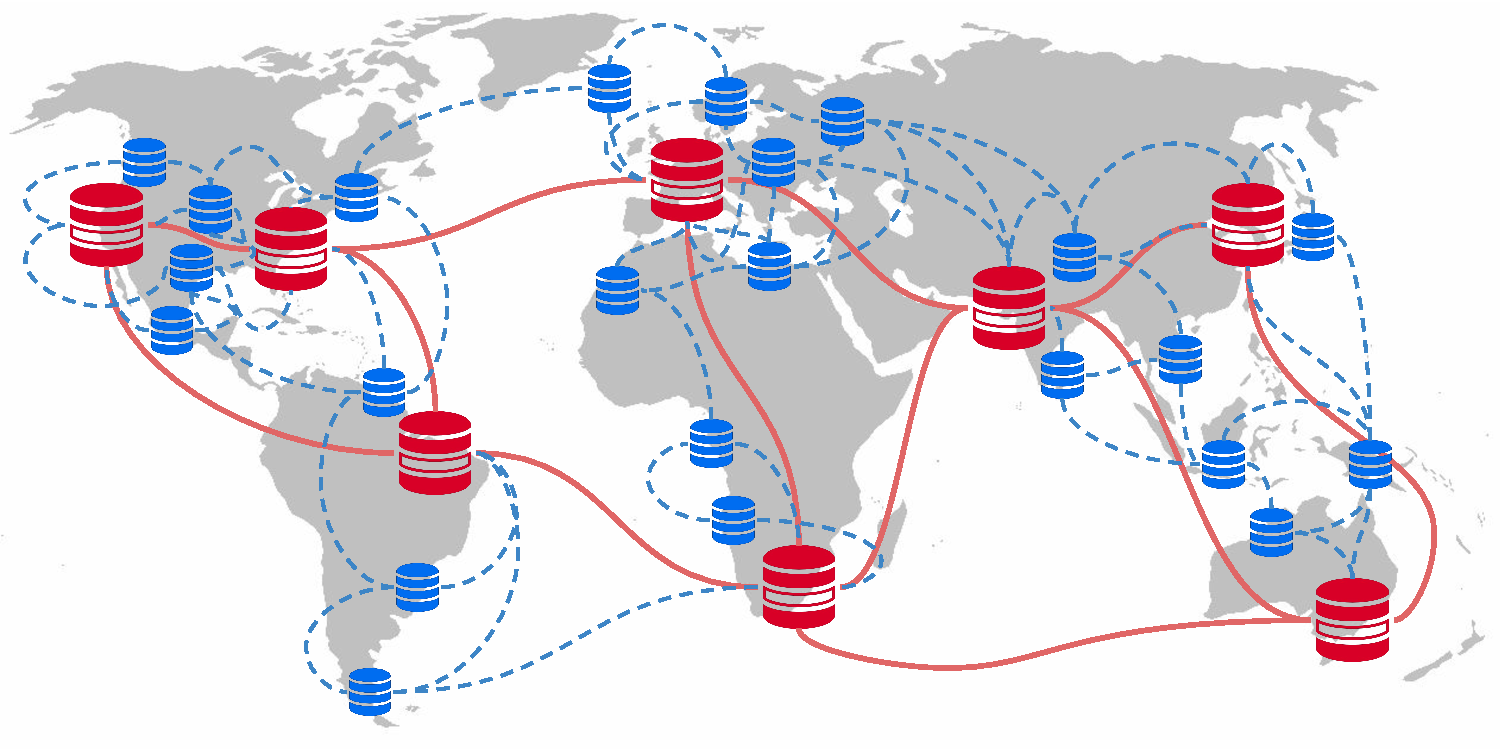
\includegraphics[width=5in]{figures/ch02_global_architecture.pdf}
    \end{center}
    \renewcommand{\baselinestretch}{1}
    \small\normalsize

    \begin{quote}
        \caption[Global Architecture]{A global architecture composed of a core backbone of hierarchical consensus replication (red) and a fog of heterogenous, federated consistency replicas (blue).}
        \label{fig:ch02_global_architecture}
    \end{quote}
\end{figure}
\renewcommand{\baselinestretch}{2}
\small\normalsize

Modern software applications require a strong consistency model that is region-agnostic.
Hierarchical consensus provides that consistency model by unifying coordination into a single-process model rather than having multiple, independent processes all coordinating accesses.
Hierarchical consensus ensures that there is an intersection between namespace coordination and access coordination so that there is a provably strong relationship between the participation of all replicas in consensus across the globe.
This relationship ensures that a general audience of developers can reason about consistency, geolocate data, and deploy systems without the complexity of most systems.

The next generation of systems will also require high-throughput writes from a mobile, heterogenous network.
Rather than relying on the centralizing effect of the cloud, we also propose to augment our system with a decentralized fog of highly available replicas.
These replicas use traditional eventually consistent systems to ensure high-availability for writes at the cost of a high likelihood of stale reads.
We propose that this outer edge layer is not independent of the centralized applications, but rather we propose a federation of consistency models that increases global consistency.
Federated consistency allows replicas to choose at which consistency level they participate in the system, creating a continuous, hybrid consistency across independent objects.

The base application we have constructed is a key/value store as described in Chapter~\ref{ch:system_implementation}.
Keys serve as the basis for sharding in our system and allow us to generically apply dependency relationships depending on the application.
Key/value stores can be seen as the underlying storage for databases, but we target two other applications: a distributed ledger and a file system.
Distributed ledgers have recently grown in popularity thanks to decentralized blockchain protocols~\cite{fruitchains}.
Hierarchical consensus can be used to quickly export a per-object or multi-object distributed log.
Key/value stores can also be used for underlying file systems~\cite{s3}.
Many high-performance distributed databases rely on an underlying replicated file system~\cite{aurora,btrdb,bigtable,megastore,spanner}.
We believe that a planet-scale file system will therefore provide the best platform to construct a myriad of services that are themselves planet-scale.

\section{Conclusion}
\label{ch02_conclusion}

In this chapter we have presented the challenges, motivations, and background of today's geo-replicated data systems.
Modern software systems are now developed with international audiences in mind, largely due to the success of large Internet companies that provide cloud infrastructure around the world.
As the demand for global-scale software has grown, so to has the need for geo-replicated services, however, while cloud providers have provided access to provisioned large scale databases, these database have been specialized and optimized for the applications they were built for, not a general audience.
The result is that software developers have to deeply consider consistency and localization semantics at the application level, which leads to confusion.

The challenge is that the current generation of geo-distributed systems rely on a pristine data-center environment, able to support a multi-process architecture on high-performance machines and networks.
Multi-process architectures have multiple levels of coordination and replication, making it extremely difficult to reason about the consistency model.
Moreover, the next generation of geo-distributed system will not reside in data-centers, but in more variable, mobile network environments.
To accommodate both of these trends, we have proposed a consistency-centric architecture for planet-scale systems.

The primary challenges for a planet-scale systems are their scale and the variability of the connections between participants.
Our architecture places primary importance on durability, fault-tolerance, heterogeneity, and adaptability by specifying two federated tiers of access.
The first tier, inside of data centers, uses hierarchical consensus to provide strong geo-replicated consistency as well as catastrophic failure tolerance by replicating data cross zones and regions.
The second tier, at the edge in the mobile network federates a highly available system model with a strong consistency model to provide stronger global guarantees.
Finally, our system self-organizes by monitoring access patterns and the network environment, adapting to change to provide resilience over time.

In the next chapter, we will explore the core component of this dissertation: hierarchical consensus.

%Chapter 3

\renewcommand{\thechapter}{3}

\chapter{Hierarchical Consensus}
% Overview, details, consistency, performance, lessons learned.

% This paragraph sucks.
The backbone of our planetary scale data system is \emph{hierarchical consensus}.
Hierarchical consensus provides a strong consistency foundation that totally orders critical accesses and arbitrates the eventual consistency layer in the fog, which raises the overall consistency of the system.
To be effective, an externalizable view of consistency ordering must be available to the entire system.
This means that strong consistency must be provided across geographic links rather than provided as localized, independent decision making with periodic synchronization.
The problem that hierarchical consensus is therefore designed to solve is that of distributed consensus.

Solutions to distributed consensus primarily focus on providing high throughput, low latency, fault tolerance, and durability.
Current approaches \cite{epaxos,mencius,calvindb,spaxos,sutra_fast_2011,peluso_making_2016} usually assume a small number of replicas, each centrally located on a highly available, powerful, and reliable host.
These assumptions are justified by the environments in which they run: highly curated environments of individual data centers connected by dedicated networks.
Although replicas in these environments may participate in global consensus, our data model requires us to accommodate replicas with heterogenous capabilities and usage modalities.
Widely distributed replicas might have neither high bandwidth nor low latency and might suffer partitions of varying durations.
Such systems of replicas might also be dynamic in membership, in relative locations, and have relative workloads.
Most importantly, to provide a backbone for a planetary scale data system, the consistency backbone must scale to include potentially hundreds of replicas around the world.

As a result, straightforward approaches of running variants of Paxos~\cite{paxos}, ePaxos~\cite{epaxos}, or Raft~\cite{raft} across the wide area, even for individual objects will perform poorly for several reasons.
First, distance (in network connectivity) between consensus replicas and the most active replicas decrease the performance of the entire system, consensus is only as fast as the final vote required to make a decision, even when making thrifty requests.
Second, network partitions are common, which cause consensus algorithms to fail-stop~\cite{fail-stop} if they cannot receive a majority, a criticism that is often used to justify eventual consistency systems for high availability.
Finally, the fault tolerance of small quorum algorithms can be disrupted by a small number of unreliable hosts and given the scale of the system and the heterogenous nature of replicas, the likelihood of individual failure is so high so as to be considered inevitable.

% what about spanner, mdcc, and calvin?

We propose another approach to building large systems.
Rather than relying on a few replicas to provide consensus to many clients, we propose to run a consensus protocol across replicas running at or near all of these locations.
The key insight is that large problem spaces can often be partitioned into mostly disjoint sets of activity without violating consistency.
We exploit this decomposition property by making our consensus protocol hierarchical and individual consensus groups fast by ensuring they are small.
We exploit locality by building subquorums from colocated replicas, and locating subquorums near clients they serve.

In this chapter we describe hierarchical consensus, a two-tiered consensus structure that allows high throughput, localization, agility, and linearizable access to a shared namespace. We show how to use \emph{delegation} to build large consensus groups that retain their fault tolerance properties while performing like small groups. We describe the use of \emph{fuzzy epoch transitions} to allow global re-configurations across multiple consensus groups without forcing them into lockstep. Finally, we describe how we reason about consistency by describing the structure of grid consistency.

\section{Overview}

Hierarchical Consensus (HC) is an implementation and extension of Vertical Paxos~\cite{vertical_paxos,boxwood,niobe} designed to scale to hundreds of nodes geo-replicated around the world.
Vertical Paxos divides consensus decisions both horizontally, as sequences of consensus instances, and vertically as individual consensus decisions are made.
Spanner~\cite{spanner}, MDCC~\cite{mdcc}, and Calvin~\cite{calvindb}, can all be thought of as implementations of Vertical Paxos, in that they shard the namespace of the objects they manage into individual consensus groups (the vertical division).
In these cases, however, sharding does not allow for inter-object dependence (the horizontal division) without either a management quorum which is either not geo-replicated, suffers from the same problems in scaling, or without the use of extremely accurate timestamps.
The challenge is therefore in building a multi-group coordination protocol that configures and mediates the subquorums with the same level of consistency and fault tolerance of the entire system.

\begin{figure}
    \begin{center}
        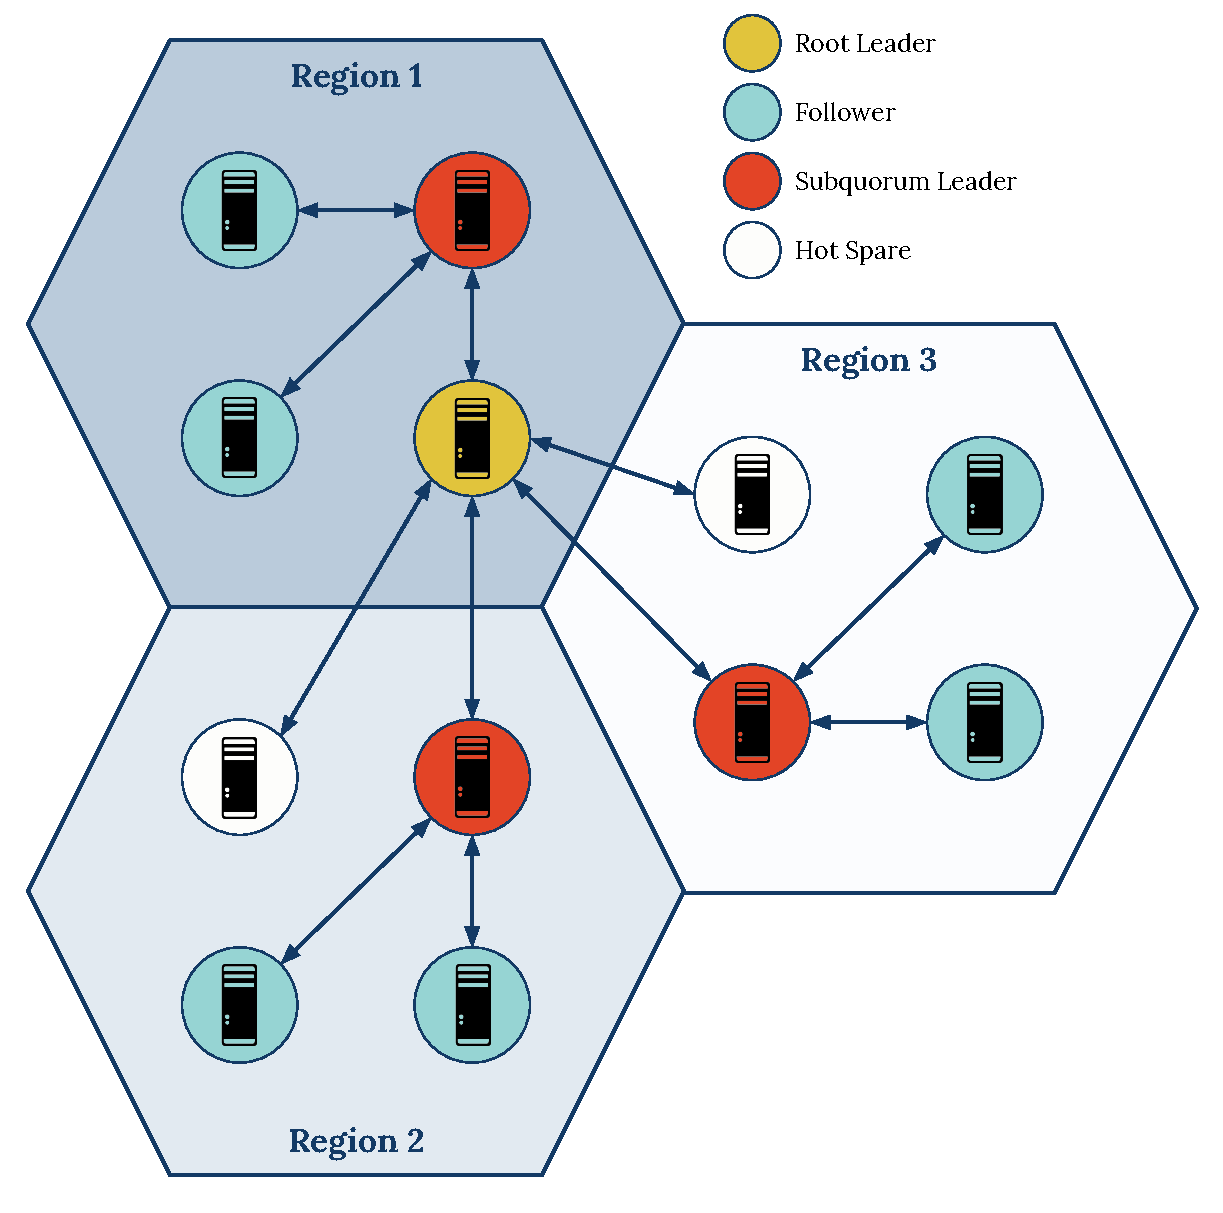
\includegraphics[width=5in]{figures/ch03_hierarchical_topology.pdf}
    \end{center}
    \renewcommand{\baselinestretch}{1}
    \small\normalsize

    \begin{quote}
        \caption[A 12x3 Hierarchical Consensus Network Topology]{A simple example of an HC network composed of 12 replicas with size 3 subquorums. Each region hosts its own subquorum and subquorum leader, while the subquorum leaders delegate their votes to the root quorum, whose leader is found in region 1. This system also has 2 hot spares that can be used to quickly reconfigure subquorums that experience failures. The hot spares can either delegate their vote, or participate directly in the root quorum.}
        \label{fig:ch03_hierarchical_topology}
    \end{quote}
\end{figure}
\renewcommand{\baselinestretch}{2}
\small\normalsize

Hierarchical consensus therefore organizes \emph{all} participating replicas to participate in a root quorum as shown in Figure~\ref{fig:ch03_hierarchical_topology}.
The root quorum guarantees correctness by pivoting the overall system through two primary functions.
First, the root quorum reconfigures subquorum memberships on replica failures and system membership changes (allocating hot-spares as needed).
Second, the root quorum adjusts the mapping of the object namespace to the underlying partitions.
Much of the system's complexity comes from handshaking between the root quorum and the lower-level subquorums during reconfigurations.

These handshakes are made easier, and much more efficient, by using \emph{fuzzy transitions}.
Fuzzy transitions allow individual subquorum to move through reconfiguration at their own pace, allowing portions of the system to transition to decisions made by the root quorum before others.
Given out heterogenous, wide-area environment, forcing the entire system to transition to new configurations in lockstep would be unacceptably slow.
Fuzzy transitions also ensure that there is no dedicated shard-master that has to synchronize all namespace allocations: at the cost of possibly multiple  redirections, clients can be redirected by any member of the root quorum to replicas who should be participating in consensus decisions for the requested objects.

Fuzzy transitions ensure that root quorum decisions need not be timely since those decisions do not disrupt accesses of clients.
Though root quorum decisions are rare with respect to the throughput of accesses inside the entire system, they still do require the participation of all members of the system, which could lead to extremely large quorum sizes, and therefore extremely slow consensus operations that may be extremely sensitive to partitions.
Because all subquorums make disjoint decisions and because all members of the system are part of the root quorum, we propose a safe relaxation of the participation requirements for the root quorum such that subquorum followers can \emph{delegate} their root quorum votes to their leader.
Delegation ensures that only a small number of replicas participate in most root quorum decisions, though decisions are made for the entire system.

In brief, the resulting system is local, in that replicas serving clients can be located near them.
The system is fast because individual operations are served by small groups of replicas, regardless of the total size of the system.
The system is nimble in that it can dynamically reconfigure the number, membership, and responsibilities of subquorums in response to failures, phase changes in the driving applications, or mobility among the member replicas.
Finally, the system is consistent, supporting the strongest form of per-object consistency without relying on special-purpose hardware~\cite{fawn,corfu,vcorfu,tango,spanner}.

\begin{figure}
    \begin{center}
        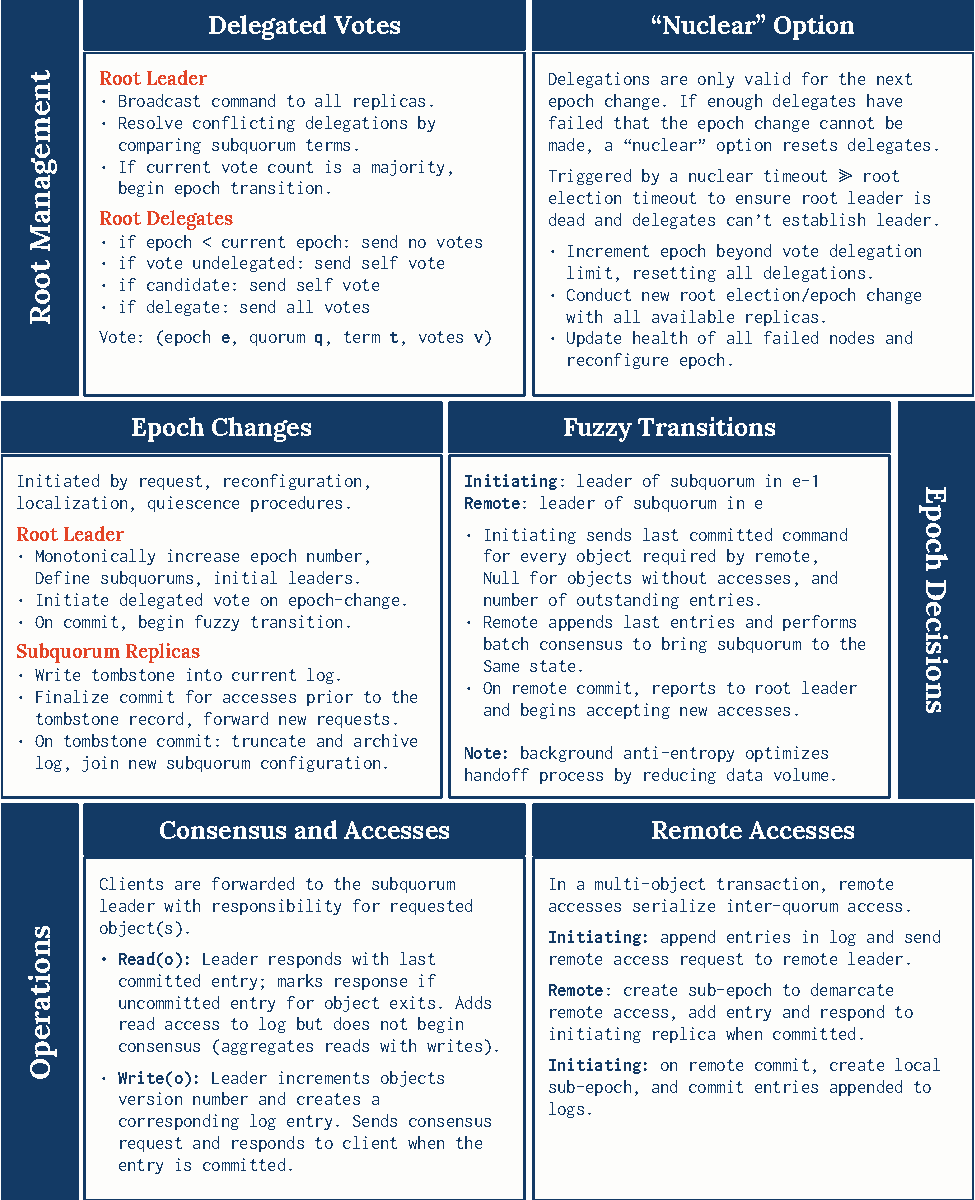
\includegraphics[width=5in]{figures/ch03_hc_operation_summary.pdf}
    \end{center}
    \renewcommand{\baselinestretch}{1}
    \small\normalsize

    \begin{quote}
        \caption[HC Operational Summary]{A condensed summary of the hierarchical consensus protocol. Operations are described in a top-to-bottom fashion where the top level is root quorum operations, the bottom is subquorum operations, and the middle is transition and intersection.}
        % Section numbers such as §5.2 indicate where particular features are discussed.
        \label{fig:ch03_hc_operation_summary}
    \end{quote}
\end{figure}
\renewcommand{\baselinestretch}{2}
\small\normalsize

A complete summary of hierarchical consensus is described in Figure~\ref{fig:ch03_hc_operation_summary}.

\section{Consensus}

The canonical distributed consensus used by systems today is Paxos~\cite{paxos,paxos_simple}.
Paxos is provably safe and designed to make progress even when a portion of the system fails.
Raft~\cite{raft} was designed not to improve performance, but to increase understanding of consensus behavior to better allow efficient implementations.
HC uses Raft as a building block, so we describe the relevant portions of Raft at a high level, referring the reader to the original paper for complete details.
Though we chose to base our protocol on Raft, a similar approach could be used to modify Paxos into a hierarchical structure.

Consensus protocols typically have two phases: leader \emph{election} and operations \emph{commit}\renewcommand{\baselinestretch}{1} \small\footnotesize\footnote{Election and commit phases correspond to PROPOSE and ACCEPT phases in Paxos}\renewcommand{\baselinestretch}{2} \small\normalsize.
Raft is a strong-leader consensus protocol, which allows the election phase to be elided while a leader remains available.
The protocol requires only a single communication round to commit an operation in the common case.
Raft uses timeouts to trigger phase changes and provide fault tolerance.
Crucially, it relies on timeouts only to provide progress, not safety.
New elections occur when another replica in the quorum times out waiting for communication from the leader.
Such a replica increments its \emph{term} until it is greater than the existing leader, and announce its candidacy.
Other replicas vote for the candidate if they have not seen a competing candidate with a larger term.
During regular operation, clients send requests to the leader, which broadcasts \texttt{AppendEntries} messages carrying operations to all replicas.
An operation is \emph{committed} and can be executed when the leader receives acknowledgments of the \texttt{AppendEntries} message from more than half the replicas (including itself).

\todo{We describe differences in our Raft implementation from the canonical implementation in Chapter~\ref{ch:system_implementation}}

Throughout the rest of this chapter we use the term \emph{root quorum} to refer to the upper, namespace-mapping and configuration-management tier of HC, and \emph{subquorum} to describe a group of replicas (called \emph{peers}) participating in consensus decisions for a section of the namespace.
The root quorum shepherds subquorums through \emph{epochs}, each with potentially different mappings of the namespace and replicas to subquorums.
An epoch corresponds to a single commit phase of the root quorum.
We use the term Raft only when describing details particular to our current use of Raft as the underlying consensus algorithm.
We refer to the two phases of the base consensus protocol as the \emph{election phase} and the \emph{commit phase}.
We use the term \emph{vote} as a general term to describe positive responses in either phase.
Epoch $x$ is denoted $e_x$.
Subquorum $i$ of epoch $e_x$ is represented as $q_{i,x}$, or just $q_i$ when the epoch is obvious.
$t_a$ represents a specific \emph{tag}, or disjoint subset of the namespace.

We assume faults are fail-stop~\cite{fail-stop} rather than Byzantine~\cite{byzantine-generals}.
We do not assume that either replica hosts or networks are homogeneous, nor do we assume freedom from partitions and other network faults.


\subsection{Root Consensus}

\begin{figure}
    \begin{center}
        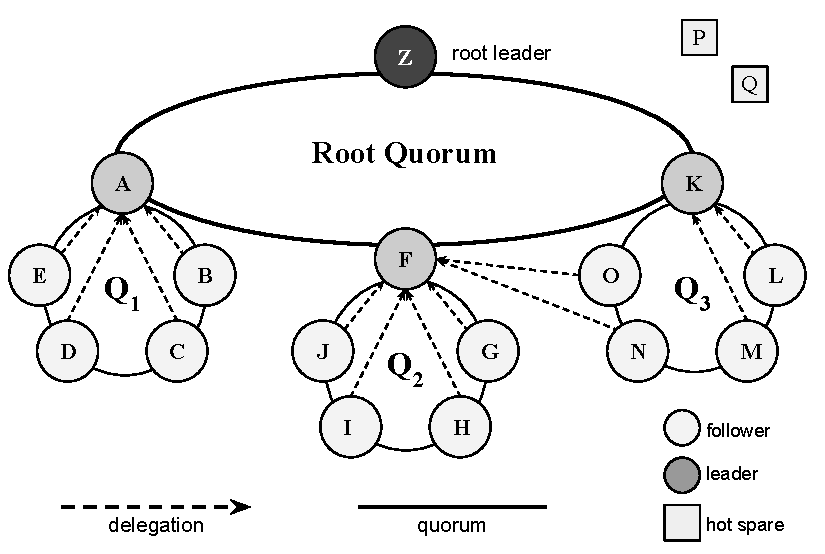
\includegraphics[width=5in]{figures/ch03_election.pdf}
    \end{center}
    \renewcommand{\baselinestretch}{1}
    \small\normalsize

    \begin{quote}
        \caption[Delegated Votes]{}
        \label{fig:ch03_tiers}
    \end{quote}
\end{figure}
\renewcommand{\baselinestretch}{2}
\small\normalsize

Hierarchical consensus is a leader-oriented protocol that organizes replicas into two tiers of quorums, each responsible for fundamentally different decisions (Figure~\ref{fig:ch03_tiers}).
The lower tier consists of multiple independent subquorums, each committing operations to local shared logs.
The upper,  \emph{root quorum}, consists of subquorum peers, usually their leaders, delegated to represent the subquorum in root elections and commits.
Hierarchical consensus's main function is to export a linearizable abstraction of shared accesses to some underlying substrate, such as a distributed object store or file system.
We assume that nodes hosting object stores, applications, and HC are frequently co-located across the wide area.

The root quorum's primary responsibilities are mapping namespaces and replicas to individual subquorums.
Each such map defines a distinct epoch, $e_i$, a monotonically increasing representation of the term of $q_{i,e}$.
The root quorum is effectively a consensus group consisting of subquorum leaders.
Somewhat like subquorums, the effective membership of the root quorum is not defined by the quorum itself, but in this case by leader election or peer delegations in the lower tier.

The root quorum partitions the namespace across multiple subquorums, each with a disjoint portion as its scope.
The intent of subquorum localization is ensure that the \emph{domain} of a client, the portion of the namespace it accesses, is entirely within the scope of a local, or nearby, subquorum.
If true across the entire system, each client interacts with only one subquorum, and subquorums do not interact at all during execution of a single epoch.
This \emph{siloing} of client accesses simplifies implementation of strong consistency guarantees and allows better performance.

\subsection{Delegation}

Fault tolerance scales with increasing system size.
The root quorum's membership is, at least logically, the set of all system replicas, at all times.
However, running consensus elections across large systems is inefficient in the best of cases, and prohibitively slow in a geo-replicated environment.
Root quorum decision-making is kept tractable by having replicas \emph{delegate} their votes, usually to their leaders, for a finite duration.
With leader delegation, the root membership effectively consists of the set of subquorum leaders.
Each leader votes with a count describing its own and peer votes from its
subquorum.

Consider an alternative leader-based approach where root quorum membership is defined as the current set of subquorum leaders.
Both delegation and the leader approach have clear advantages in performance and flexibility over direct votes of the entire system.
However, the leader approach dramatically decreases fault tolerance.
Furthermore, the root quorum becomes unstable in the leader approach as its membership changes during partitions or subquorum elections.
% Furthermore, \roo membership changes with \sub leaders and at \sub
% repartitions in the leader approach.
These changes would require heavyweight \emph{joint consensus} decisions in the root quorum for correctness in Raft-like protocols~\cite{raft}.

With delegation, however, root quorum membership is always the entire system and remains unchanged over subquorum re-configuration.
Delegation is essentially a way to optimistically shortcut contacting every replica for each decision.
Subquorum repartitioning merely implies that a given replica's vote might need to be delegated to a different leader.

Delegation does add one complication: the root quorum leader must know all vote delegations to request votes when committing epoch changes.
We deal with this issue, as well as the requirement for a nuclear option (Section~\ref{sec:nuclear}), by simplifying our protocol.
Instead of sending vote requests just to subquorum leaders, \textbf{the root quorum leader sends vote requests to all system replicas.}
This is true even for \emph{hot spares}, which are not currently in any subquorum.

This is correct because vote requests now reach all replicas, and because replicas whose votes have been delegated merely ignore the request.
We argue that it is also efficient, as a commit's efficiency depends only on receipt of a majority of the votes.
Large consensus groups are generally slow (see Section~\ref{sec:evaluation}) not just because of communication latency, but because large groups in a heterogeneous setting are more likely to include replicas on very slow hosts or networks.
In the usual case for our protocol, the root leader still only needs to wait for votes from the subquorum leaders.
Leaders are generally those that respond more quickly to timeouts, so the
speed of root quorum operations is unchanged.
% Not generally true, as timeouts are stochastic.

\subsection{Epoch Transitions}

% - tagspace (prefix-trie)
% - fuzzy transitions
% - anti-entropy and tombstones

An epoch change is initiated by the leader in response to one of several events, including:

\renewcommand{\baselinestretch}{1}
\begin{itemize}
    \item a namespace repartition request from a subquorum leader
    \item notification of join requests by new replicas
    \item notification of failed replicas
    \item changing network conditions that suggest re-assignment of replicas
\end{itemize}
\renewcommand{\baselinestretch}{2}

The root leader transitions to a new epoch through the normal commit phase in the root quorum.
The command proposed by the leader is an enumeration of the new subquorum partition, namespace partition, and assignment of namespace portions to specific subquorums.
The announcement may also include initial leaders for each subquorum, with the usual rules for leader election applying otherwise, or if the assigned leader is unresponsive.
Upon commit, the operation serves as an \emph{announcement} to subquorum leaders.
Subquorum leaders repeat the announcement locally, disseminating full knowledge of the new system configuration, and eventually transition to the new epoch by committing an \texttt{epoch-change} operation locally.

The epoch change is lightweight for subquorums that are not directly affected by the underlying re-configuration.
If a subquorum is being changed or dissolved, however, the \emph{epoch-change} commitment becomes a tombstone written to the logs of all local replicas.
No further operations will be committed by that version of the subgroup, and the local shared log is archived and then truncated.
Truncation is necessary to guarantee a consistent view of the log within a subquorum, as peers may have been part of different subquorums, and thus have different logs, during the last epoch.
Replicas then begin participating in their new subquorum instantiation.
In the common case where a subquorum's membership remains unchanged across the transition, an \texttt{epoch-change} may still require additional mechanism because of changes in namespace responsibility.

\begin{landscape}
\begin{figure}
    \begin{center}
        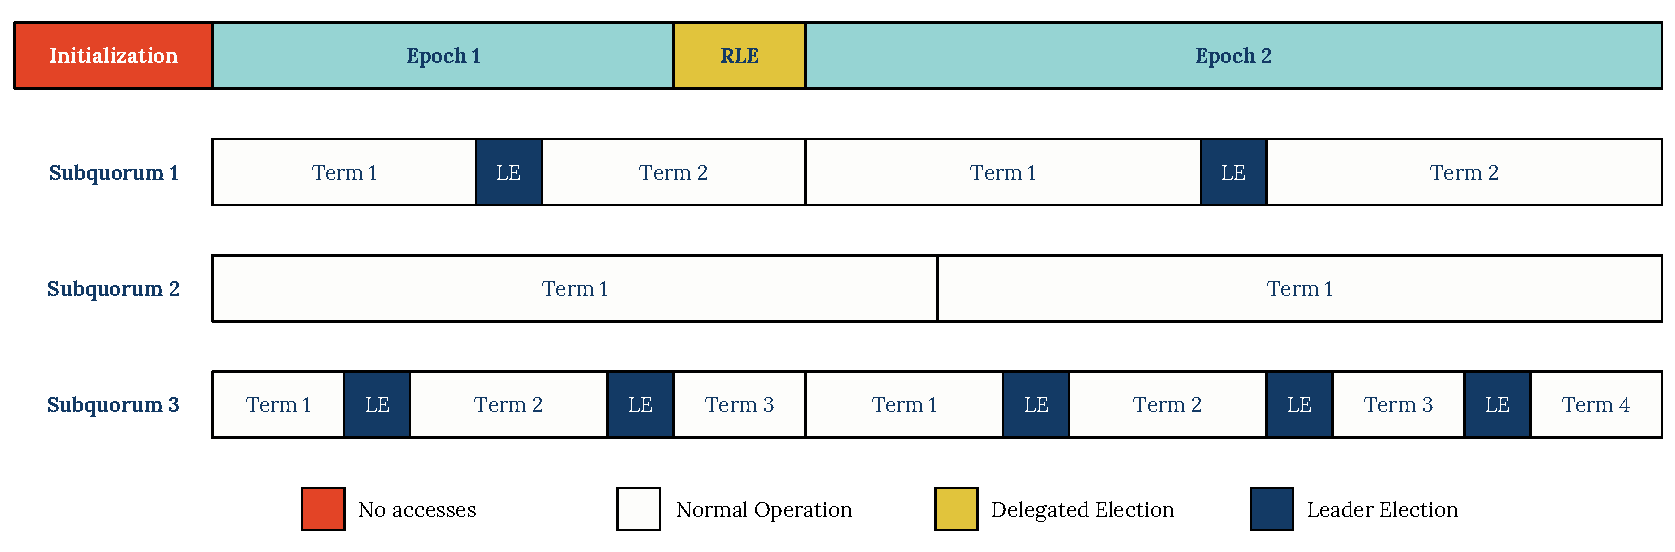
\includegraphics[width=8.2in]{figures/ch03_epochs_terms.pdf}
    \end{center}
    \renewcommand{\baselinestretch}{1}
    \small\normalsize

    \begin{quote}
        \caption[Ordering of Epochs and Terms in Root and Subquorums]{}
        \label{fig:ch03_epochs_terms}
    \end{quote}
\end{figure}
\renewcommand{\baselinestretch}{2}
\small\normalsize
\end{landscape}

\subsection{Fuzzy Handshakes}

Epoch handshakes are required whenever the namespace-to-subquorum mapping changes across an epoch boundary.
HC separates epoch transition announcements in the root quorum from implementation in subquorums.
Epoch transitions are termed \emph{fuzzy} because subquorums need not all transition synchronously.
There are many reasons why a subquorum might be slow.
Communication delays and partitions might delay notification.
Temporary failures might block local commits.
A subquorum might also delay transitioning to allow a local burst of activity to cease such as currently running transactions\renewcommand{\baselinestretch}{1} \small\footnotesize\footnote{The HC implementation discussed in this chapter does not currently support transactions.}\renewcommand{\baselinestretch}{2} \small\normalsize.
Safety is guaranteed by tracking subquorum dependencies across the epoch boundary.

\begin{figure}
    \begin{center}
        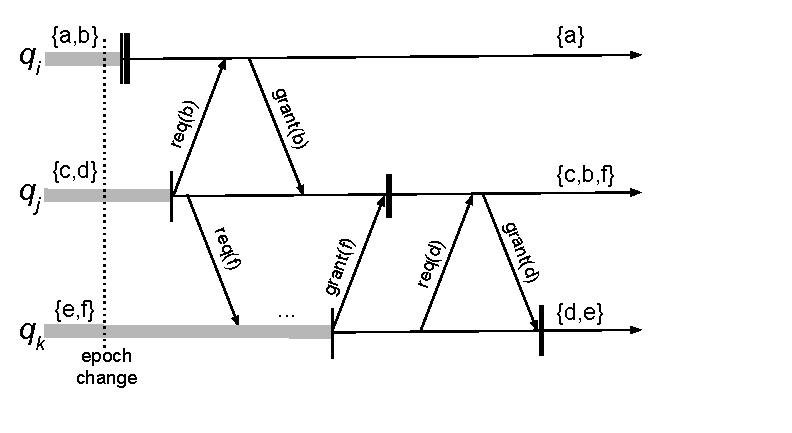
\includegraphics[width=5in]{figures/ch03_namespace_handoff.pdf}
    \end{center}
    \renewcommand{\baselinestretch}{1}
    \small\normalsize

    \begin{quote}
        \caption[Epoch Transition: Fuzzy Handshakes]{Readiness to transition to the new epoch is marked by a thin vertical bar; actual transition is the thick vertical bar.  Thick gray lines indicate operation in the previous epoch.  Subquorum $q_j$ transitions from tag ${c,d}$ to ${c,b,f}$, but begins only after receiving version information from previous owners of those tags.  The request to $q_k$ is only answered once $q_k$ is ready to transition as well.}
        \label{fig:ch03_namespace_handoff}
    \end{quote}
\end{figure}
\renewcommand{\baselinestretch}{2}
\small\normalsize

Figure~\ref{fig:ch03_namespace_handoff} shows an epoch transition where the scopes of $q_i$, $q_j$, and $q_k$ change across the transition as follows:

\todo{Fix the alignment of the below equations:}

\renewcommand{\baselinestretch}{1}
\begin{eqnarray}
    q_{i,x-1} = t_a, t_b  &\longrightarrow q_{i,x} = t_a\\
    q_{j,x-1} = t_c, t_d  &\longrightarrow q_{j,x} = t_c,t_d,t_f\\
    q_{k,x-1} = t_e, t_f  &\longrightarrow q_{k,x} = t_d,t_e
\end{eqnarray}
\renewcommand{\baselinestretch}{2}

All three subquorums learn of the epoch change at the same time, but become ready with varying delays.
These delays could be because of network lags or ongoing local activity.
Subquorum $q_i$ gains no new tags across the transition and moves immediately to the new epoch.
Subquorum $q_j$'s readiness is slower, but then it sends requests to the owners of both the new tags it acquires in the new epoch.
Though $q_i$ responds immediately, $q_k$ delays its response until locally operations conclude.
Once both handshakes are received, $q_j$ moves into the new epoch, and $q_k$ later follows suit.

These bilateral handshakes allow an epoch change to be implemented incrementally, eliminating the need for lockstep synchronization across the entire system.
This flexibility is key to coping with partitions and varying connectivity in the wide area.
However, this piecewise transition, in combination with subquorum re-definition and configuration at epoch changes, also means that individual replicas \emph{may be part of multiple subquorums at a time}.

This overlap is possible because replicas may be mapped to distinct subgroups from one epoch to the next.
Consider $q_k$ in Figure~\ref{fig:ch03_namespace_handoff} again.
Assume the epochs shown are $e_x$ and $e_{x+1}$.
A single replica, $r_a$, may be remapped from subquorum $q_{k,x}$ to subquorum $q_{i,x+1}$ across the transition.
Subquorum $q_{k,x}$ is late to transition, but $q_{i,x+1}$ begins the new epoch almost immediately.
Requiring $r_a$ to participate in a single subquorum at a time would potentially delay $q_{i,x+1}$'s transition and impose artificial synchronicity constraints on the system.
One of the many changes we made in the base Raft protocol is to allow a replica to have multiple distinct shared logs.
Smaller changes concern the mapping of requests and responses to the appropriate consensus group.

\subsection{Subquorum Consensus}

\todo{this section is bad}

Each subquorum, $q_i$, elects a leader to coordinate local decisions.
Fault tolerance of the subquorum is maintained in the usual way, detecting leader failures and electing new leaders from the peers.
Subquorums do not, however, ever change system membership on their own.
Subquorum membership is always defined in the root quorum.

Subquorum consensus is used to commit object writes.
Reads are not committed by default, but are always served by the leader of the
appropriate subquorum.
Namespace assignments in HC result in the object space being partitioned (or
sharded) across distinct subqourms.
The mapping of the shared object namespace to individual subquorums is the
\emph{tagset}, or the tagset partition.
An individual \emph{tag} defines a disjoint subset of the object space.

As writes are committed through HC, the shared logs provide a complete version history of all distributed objects.
Subquorum leaders use in-core caches to provide fast access to recently accessed objects in the local subquorums's tag.
Replicas perform background anti-entropy~\cite{dynamo,bayou,anti_entropy}, disseminating log updates a user-defined number of times across the system.

The most complex portion of the HC protocol is in handling data-related issues at epoch transitions.
Transitions may cause tags to be transferred from one subquorum to another, forcing the new leader to load state remotely to serve object requests.
Transitions handshakes are augmented in three ways.
First, an replica can demand-fetch an object version from any other system replica.
Second, epoch handoffs contain enumerations of all current object versions, though not the data itself.
Knowing an object's current version gives the new handler of a tag the ability to demand fetch an object that is not yet present locally.
Finally, handshakes start immediate fetches of the in-core version cache from the leader of the tag's subquorum in the old epoch to the leader in the new.

We do not currently gather the entire shared log onto a single replica because of capacity and flexibility issues.
Capacity is limited because our system and applications are expected to be long-lived.
Flexibility is a problem because HC, and applications built on HC, gain much of their value from the ability to pivot quickly, whether to deal with changes in the environment or for changing application access patterns.
We require handoffs to be as lightweight as possible to preserve this advantage.

\subsection{Client Operations}

\todo{- Sessions
- Connect to closest available replica, redirected to closest available leader.}

Client namespace accesses are forwarded to the leader of the subquorum for the appropriate part of the namespace.
The underlying Raft semantics ensure that leadership changes do not result in loss of any commits.
Hence, individual- or multiple-client accesses to a single subquorum are totally ordered.
\emph{Remote accesses}, or client accesses to other than their local subquorum, are transparent to the primary protocol.
However, creation of a single shared log of all system operations requires remote accesses to be logged.

\section{Consistency}

Pushing all writes through subquorum commits and serving reads at leaders allows us to guarantee that accesses are linearizable (Lin), which is the strongest non-transactional consistency~\cite{linearizability,sequential_consistency}.
As a recap, linearizability is a combination of atomicity and timeliness guarantees about accesses to a single object.
Both \texttt{reads} and \texttt{writes} must appear atomic, and also instantaneous at some time between a request and the corresponding response to a client.
\texttt{Reads} must always return the latest value.
This implies that reads return values are consistent \emph{with any observed ordering}, i.e., the ordering is \emph{externalizable}~\cite{externalizable}.

Linearizability of object accesses can be \emph{composed}.
If operations on each object are linearizable, the entire object space is also linearizable.
This allows our subquorums to operate independently while providing a globally consistent abstraction.

\subsection{Globally Consistent Logs}
\label{sec:ch03_log_ordering}

Our default use case is in providing linearizable access to an object store.
Though this approach allows us to guarantee all observers will see linearizable results of object accesses in real-time, the system is not able to enumerate a total order, or create a linearizable shared log.
Such a linear order would require fine-grained (expensive) coordination across the entire system, or fine-grained clock synchronization~\cite{spanner}.
Though many or most distributed applications (objects stores, file systems, etc.) will work directly with HC, shared logs are a useful building block for distributed systems.

HC \emph{can} be used to build a sequentially consistent (SC) shared log as shown in Figure~\ref{fig:ch03_log_ordering}.
Like Lin, SC requires all observers to see a single total ordering.
SC differs in that this total ordering does not have to be externalizable.
Instead, it merely has to conform to local operation orders and all reads-from dependencies.

\todo{write about grid consistency}

\begin{landscape}
\begin{figure}
    \begin{center}
        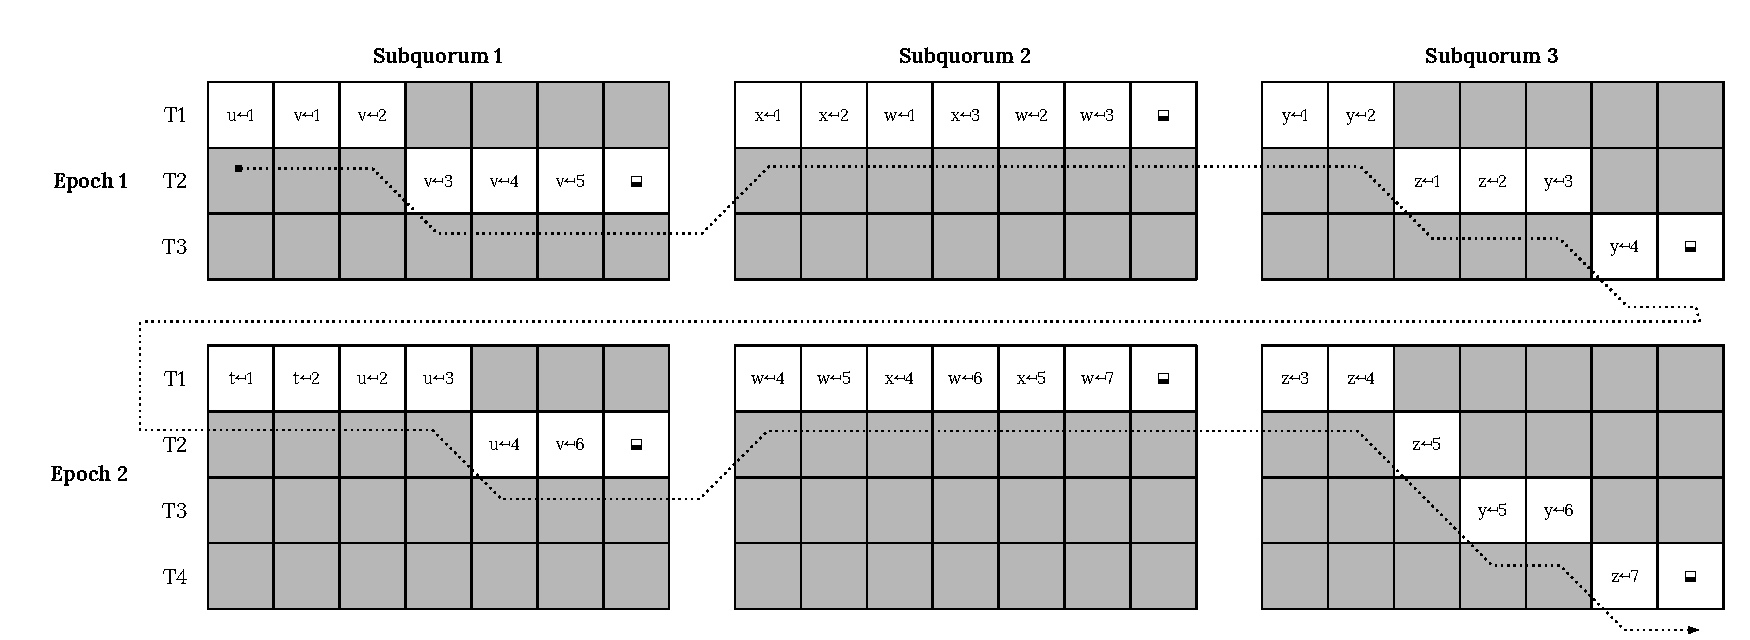
\includegraphics[width=8.2in]{figures/ch03_log_ordering.pdf}
    \end{center}
    \renewcommand{\baselinestretch}{1}
    \small\normalsize

    \begin{quote}
        \caption[Grid Consistency: A Sequential Log Ordering]{}
        \label{fig:ch03_log_ordering}
    \end{quote}
\end{figure}
\renewcommand{\baselinestretch}{2}
\small\normalsize
\end{landscape}


Figure~\ref{fig:ch03_event_ordering} shows a system with subquorums $q_i$ and $q_j$, each of which performs a pair of writes.
Dotted lines show one possible event ordering for replicas $q_i$ (responsible for objects $a$ and $b$), and $q_j$ ($c$ and $d$).
Without cross-subquorum reads or writes, ordering either
subquorums's operations first creates a SC total ordering: $q_i \rightarrow q_j$ (``happened-before''~\cite{lamport_time_1978})
implies $w_{i,1} \rightarrow w_{i,3} \rightarrow w_{j,1} \rightarrow w_{j,3}$,
for example.

\begin{figure}
    \begin{center}
        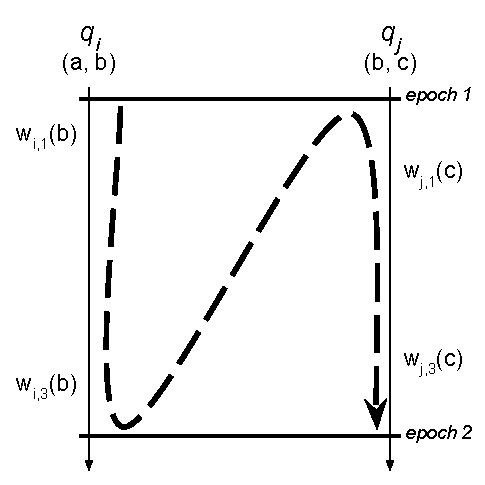
\includegraphics[width=5in]{figures/ch03_event_ordering.pdf}
    \end{center}
    \renewcommand{\baselinestretch}{1}
    \small\normalsize

    \begin{quote}
        \caption[Sequential Event Ordering in HC]{Default ordering: $w_{i,1\rightarrow w_{i,3}\rightarrow w_{j,1}\rightarrow w_{j,3}}$}
        \label{fig:ch03_event_ordering}
    \end{quote}
\end{figure}
\renewcommand{\baselinestretch}{2}
\small\normalsize

By contrast, the subquorums in Figure~\ref{fig:ch03_event_ordering_remote_write} create additional dependencies by issuing remote writes to other subquorums: $w_{i,2} \rightarrow w_{j,3}$ and $w_{j,2} \rightarrow w_{i,3}$.
Each remote write establishes a partial ordering between events of the sender before the sending of the write, and writes by the receiver after the write is received.
Similar dependencies result from remote reads.


\begin{figure}
    \begin{center}
        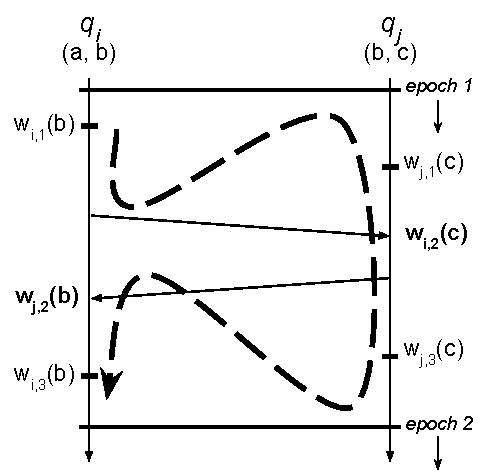
\includegraphics[width=5in]{figures/ch03_event_ordering_remote_write.pdf}
    \end{center}
    \renewcommand{\baselinestretch}{1}
    \small\normalsize

    \begin{quote}
        \caption[Event Ordering with Remote Writes in HC]{Remote writes add additional ordering constraints: $w_{i,1} \rightarrow w_{i,2}\rightarrow w_{j,3}$, and $ w_{j,1} \rightarrow w_{j,2} \rightarrow w_{i,3}$}
        \label{fig:ch03_event_ordering_remote_write}
    \end{quote}
\end{figure}
\renewcommand{\baselinestretch}{2}
\small\normalsize

These dependencies cause the epochs to be split (not shown in picture).
The receipt of write $w_{i,2}$ in $q_j$ causes $q_{j,1}$ to be split into
$q_{j,1.1}$ and $q_{j,1.2}$.
Likewise, the receipt of write $w_{j,2}$ into $q_i$ causes $q_i$ to be split
into $q_{i,1.1}$ and $q_{i,1.2}$.
Any topological sort of the subepochs that respects these orderings, such as
$q_{i,1.1} \rightarrow q_{j,1.1} \rightarrow q_{j,1.2} \rightarrow q_{i,1.2}$,
results in a valid SC ordering.

Presenting a sequentially consistent global log across the entire system, then, only requires tracking these inter-subquorum data accesses, and then performing an $\mathcal{O}(n)$ merge of the subepochs.

By definition, this log's ordering respects any externally visible ordering of cross-subquorum accesses (accesses visible to the system).
However, the log does not necessarily order other accesses according to external visibility.
The resulting shared log could not be mined to find causal relationships between accesses through external communication paths unknown to the system.

For example, assume that log events are published posts, and that one user claimed plagiarism.
The accused would not be able to prove that his post came first unless there were some causal chain of posts and references visible to the protocol.


\section{Fault Tolerance}
\label{sec:fault_tolerance}

We assert that consensus at the leaf replicas is correct and safe because decisions are implemented using well-known leader-oriented consensus approaches.
Hierarchical consensus therefore has to demonstrate linearizable correctness and safety between subquorums for a single epoch and between epochs.
Briefly, linearizability requires external observers to view operations to objects as instantaneous events.
Within an epoch, subquorum leaders serially order local accesses, thereby guaranteeing linearizability for all replicas in that quorum.
% Remote accesses and the internal invariant also enforce linearizability of accesses
% between \subs.

Epoch transitions raise the possibility of portions of the namespace being re-assigned from one subquorum to another, with each subquorum making the transition independently.
Correctness is guaranteed by an invariant requiring subquorums to delay serving newly acquired portions of the namespace until after completing all appropriate handshakes.


\begin{landscape}
\renewcommand{\baselinestretch}{1}
\small\normalsize
 \begin{table}[ht]
\caption[HC Failure Categories]{Failure categories: Peer failure is detected by missed heartbeat messages. The rest are triggered by the appropriate election timeout.}
\begin{center}
\begin{tabular}{l|l}
\hline
Failure Type & Response \\
\hline \hline
subquorum peer & request replica repartition from root quorum \\
subquorum leader & local election, request replacement from root quorum \\
root leader & root election (with delegations)\\
majority of majority of subquorums & (nuclear option) root election after delegations timed out \\
\hline
\end{tabular}
\end{center}
\label{tab:failure_categories}
\end{table}
 \renewcommand{\baselinestretch}{2}
\small\normalsize
\end{landscape}

\subsection{Failures}

During failure-free execution, the root quorum partitions the system into\ disjoint subquorums, assigns \emph{subquorum leaders}, and assigns partitions of the tagspace to subquorums.
Each subquorum coordinates and responds to accesses for objects in its assigned tagspace.
We define the system's \emph{safety} property as guaranteeing that non-linearizable (or non-sequentially-consistent, see Section~\ref{sec:ch03_log_ordering}) event orderings can never be observed.
We define the system's \emph{progress} property as the system having enough live replicas to commit votes or operations in the root quorum.

The system can suffer several types of failures, as shown in Table~\ref{tab:failure_categories}.
Failures of subquorum and root quorum leaders are handled through the normal consensus mechanisms.
Failures of subquorum peers are handled by the local leader petitioning the root quorum to re-configure the subquorum in the next epoch.
Failure of a root quorum peer is the failure of subquorum leader, which is handled as above.
Root quorum heartbeats help inform other replicas of leadership changes, potentially necessary when individual subquorums break down.

\todo{describe assasination}

HC's structure means that some faults are more important than others.
Proper operation of the root quorum requires the majority of replicas in the majority of subquorums to be non-faulty.
Given a system with $2m+1$ subquorums, each of $2n+1$ replicas, the entire system's progress can be halted with as few as $(m+1)(n+1)$ well-chosen failures.
Therefore, in worst case, the system can only tolerate: $f_{worst}=mn+m+n$ failures and still make progress.
At maximum, HC's basic protocol can tolerate up to: $f_{best} = (m+1)*n + m*(2n+1) = 3mn+m+n$ failures.
As an example, a 25/5 system can tolerate at least 8 and up to 16 failures out of 25 total replicas.
A 21/3 system can tolerate at least 7, and a maximum of 12, failures out of 21 total replicas.
Individual subquorums might still be able to perform local operations despite an impasse at the global level.

Total subquorum failure can temporarily cause a portion of the namespace to be unserved.
However, the root quorum eventually times out and moves into a new epoch with that portion assigned to another subquorum.

\subsection{Obligations Timeout}

\todo{write this section}

\subsection{The Nuclear Option}
\label{sec:nuclear}

\todo{fix this section}

Singleton consensus protocols, including Raft, can tolerate just under half of the entire system failing.
As described above, HC's structure makes it more vulnerable to clustered failures.
Therefore we define a \emph{nuclear option}, which uses direct consensus decision among all system replicas to tolerate any $f$ replicas failing out of $2f+1$ total replicas in the system.

A nuclear vote is triggered by the failure of a root leader election.
A \emph{nuclear candidate} increment's its term for the root quorum and broadcasts a request for votes to all system replicas.
The key difficulty is in preventing delegated votes and nuclear votes from reaching conflicting decisions.
Such situations might occur when temporarily unavailable subquorum leaders regain connectivity and allow a wedged root quorum to unblock.
Meanwhile, a nuclear vote might be concurrently underway.

Replica delegations are defined as intervals over specific slots.
Using local subquorum slots would fall prey to the above problem, so we define delegations as a small number (often one) of root slots, which usually correspond to distinct epochs.
During failure-free operation, peers delegate to their leaders and are all represented in the next root election or commit.
Peers then renew their delegations to their leaders by appending them to the next local commit reply.
This approach works for replicas that change subquorums over an epoch boundary, and even allows peers to delegate their votes to arbitrary other peers in the system (see replicas $r_N$ and $r_O$ in Figure~\ref{fig:ch03_tiers}).

This approach is simple and correct, but deals poorly with leader turnovers in the subquorum.
Consider a subquorum where all peers have delegated votes to their leader for the next root slot.
If that leader fails, none of the peers will be represented.
We finesse this issue by re-defining such delegations to count root elections, root commits, \emph{and} root heartbeats.
The latter means that local peers will regain their votes for the next root quorum action if it happens after to the next heartbeat.

Consider the worst-case failure situation discussed in Section~\ref{sec:fault_tolerance}: a majority of the majority of subquorums have failed.
None of the failed subquorum leaders can be replaced, as none of those subquorums have enough local peers.

The first response is initiated when a replica holding delegations (or its own vote) times out waiting for the root heartbeat.
That replica increments its own root term, adopts the prior system configuration as its own, and becomes a root candidate.
This candidacy fails, as a majority of subquorum leaders, with all of their delegated votes, are gone.
Progress is not made until delegations time out.
In our default case where a delegation is for a single root event, this happens after the first root election failure.

At the next timeout, any replica might become a candidate because delegations have lapsed (under our default assumptions above).
Such a \emph{nuclear} candidate increments its root term and sends candidate requests to all system replicas, succeeding if it gathers a majority across all live replicas.

The first candidacy assumed the prior system configuration in its candidacy announcement.
This configuration is no longer appropriate unless some of the ``failed'' replicas quickly regain connectivity.
Before the replica announces its candidacy for a second time, however, many of the replica replies have timed out.
The candidate alters its second proposed configuration by recasting all such replicas as hot spares and potentially reducing the number and size of the subgroups.
Subsequent epoch changes might re-integrate the new hot spares if the replicas regain connectivity.

\section{Performance Evaluation}
\label{sec:evaluation}

HC was designed to adapt both to dynamic workloads as well as variable network conditions.
We therefore evaluate HC in two distinct environments: a homogeneous data center and a heterogeneous real-world network.
The homogeneous cluster is hosted on Amazon EC2 and includes 26 ``t2.medium'' instances: dual-core virtual machines running in a single VPC with inter-machine latencies of $\lambda_{\mu}=0.399ms$ and $\lambda_{\sigma}=0.216ms$.
These machines are cost effective and, though lightweight, are easy to scale to large cluster sizes as workload increases.
Experiments are set up such that each instance runs a single replica process and multiple client processes.

The heterogeneous cluster (UMD) consists of several local machines distributed across a wide area, with inter-machine latencies ranging from
$\lambda_{\mu}=2.527ms$,
$\lambda_{\sigma}=1.147ms$ to $\lambda_{\mu}=34.651ms$,
$\lambda_{\sigma}=37.915ms$.
Machines in this network are a variety of dual and quad core desktop servers that are solely dedicated to running these benchmarks.
Experiments on these machines are set up so that each instance runs multiple replica and client processes co-located on the same host.
In this environment, localization is critical both for performance but also to ensure that the protocol can elect and maintain consensus leadership.
The variability of this network also poses challenges that HC is uniquely suited to handle via root quorum-guided adaptation.
We explore two distinct scenarios -- sawtooth and repartitioning -- using this cluster; all other experiments were run on the EC2 cluster.

\begin{figure}
    \begin{center}
        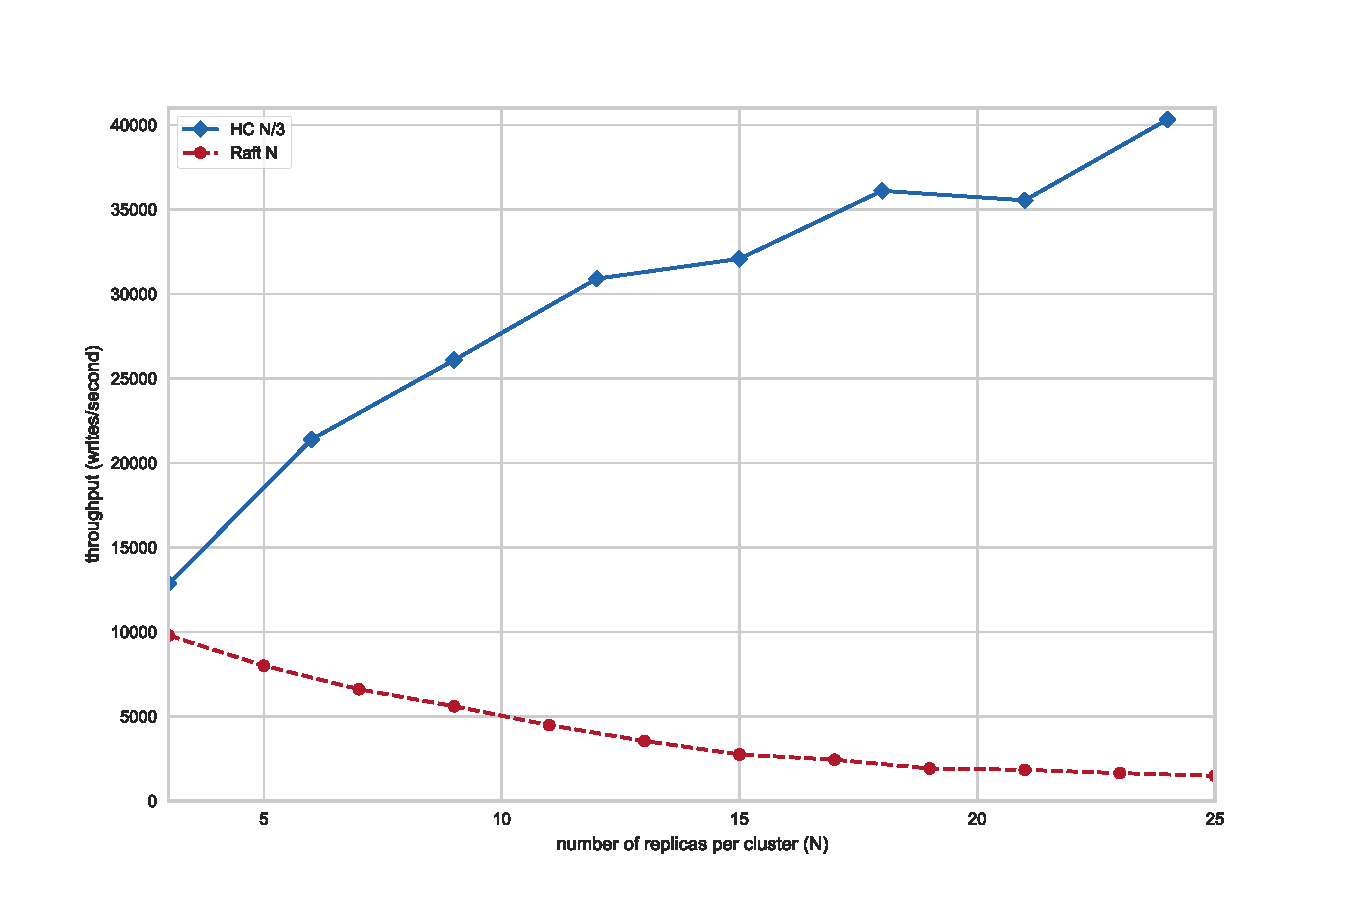
\includegraphics[width=5in]{figures/ch03_scaling_consensus.pdf}
    \end{center}
    \renewcommand{\baselinestretch}{1}
    \small\normalsize

    \begin{quote}
        \caption[Scaling Consensus HC vs. Raft]{Mean throughput of workloads of up to 120 concurrent clients}
        \label{fig:ch03_scaling_consensus}
    \end{quote}
\end{figure}
\renewcommand{\baselinestretch}{2}
\small\normalsize

HC is partially motivated by the need to scale strong consistency to large cluster sizes.
We based our work on the assumption that consensus performance decreases as the quorum size increases, which we confirm empirically in Figure~\ref{fig:ch03_scaling_consensus}.
This figure shows the maximum throughput against system size for a variety of workloads, up to 120 concurrent clients.
A workload consists of one or more clients continuously sending writes of a specific object or objects to the cluster without pause.

Standard consensus algorithms, Raft in particular, scale poorly with uniformly decreasing throughput as nodes are added to the cluster.
Commit latency increases with quorum size as the system has to wait for more responses from peers, thereby decreasing overall throughput.
Figures~\ref{fig:ch03_scaling_consensus} and~\ref{fig:ch03_hc_throughput_workload} clearly show the multiplicative advantage of HC's hierarchical structure, though HC does not scale linearly as we had expected.

\begin{figure}
    \begin{center}
        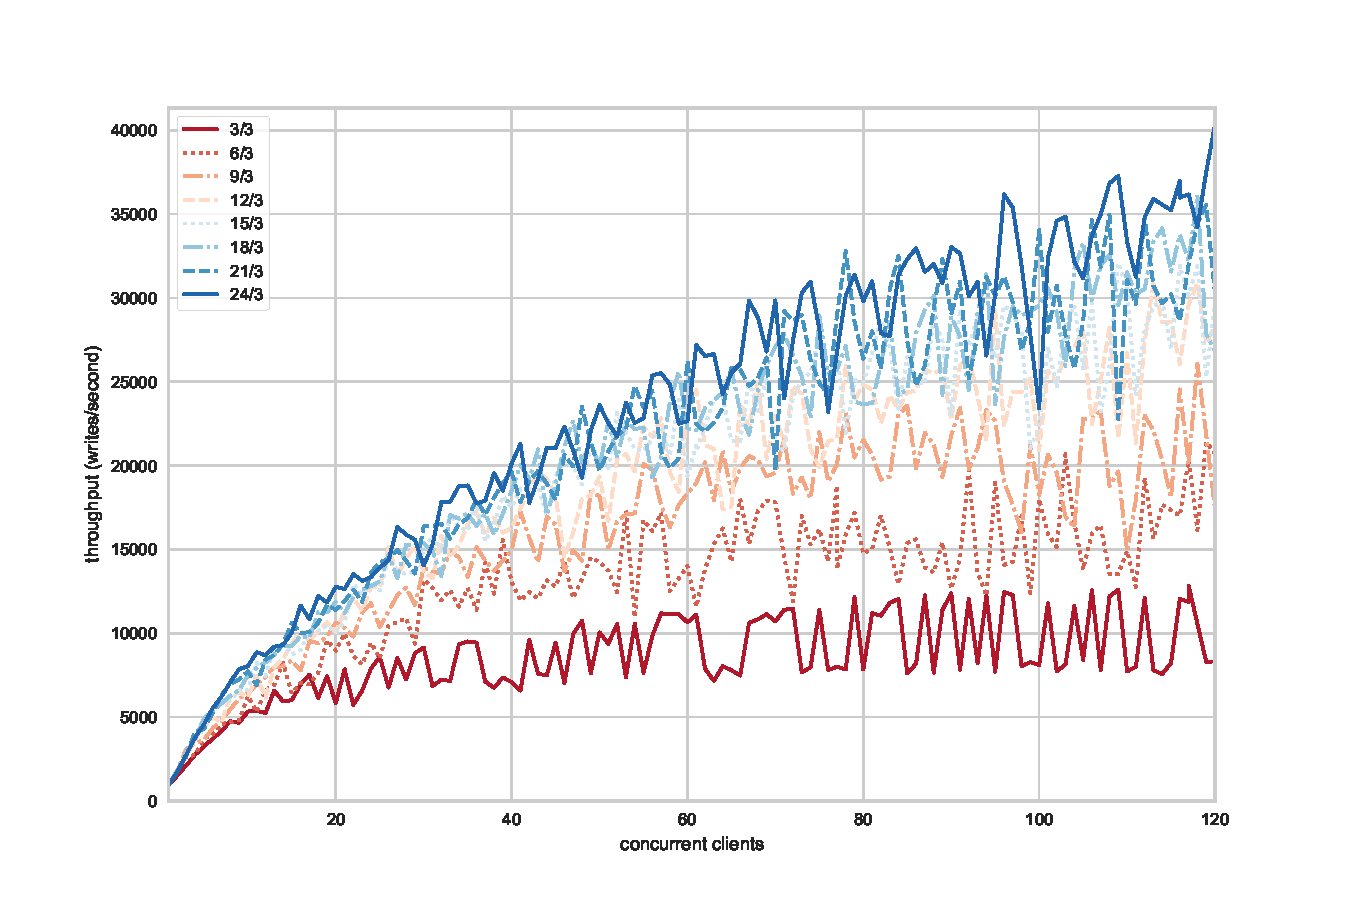
\includegraphics[width=5in]{figures/ch03_hc_throughput_workload.pdf}
    \end{center}
    \renewcommand{\baselinestretch}{1}
    \small\normalsize

    \begin{quote}
        \caption[HC Throughput vs. Workload in the Wide Area]{Performance of distributed consensus with an increasing workload of concurrent clients. Performance is measured by throughput, the number of writes committed per second.}
        \label{fig:ch03_hc_throughput_workload}
    \end{quote}
\end{figure}
\renewcommand{\baselinestretch}{2}
\small\normalsize

There are at least two factors currently limiting the HC throughput shown here.
First, the HC subquorums for the larger system sizes are not saturated.
A single 3-node subquorum saturates at around 25 clients and this experiment has only about 15 clients per subquorum for the largest cluster size.
We ran experiments with 600 clients, saturating all subquorums even in the 24-node case.
This throughput peaked at slightly over 50,000 committed writes per second, better but still lower than the linear scaling we had expected.

We think the reason for this ceiling is hinted at by Figure~\ref{fig:ch03_hc_throughput_workload}.
This figure shows increasingly larger variability with increasing system sizes.
A more thorough examination of the data shows widely varying performance across individual subquorums in the larger configurations.
We suspect that the cause is either VM misconfiguration or misbehavior.
We are adding more instrumentation to diagnose the problem.

\begin{figure}
    \begin{center}
        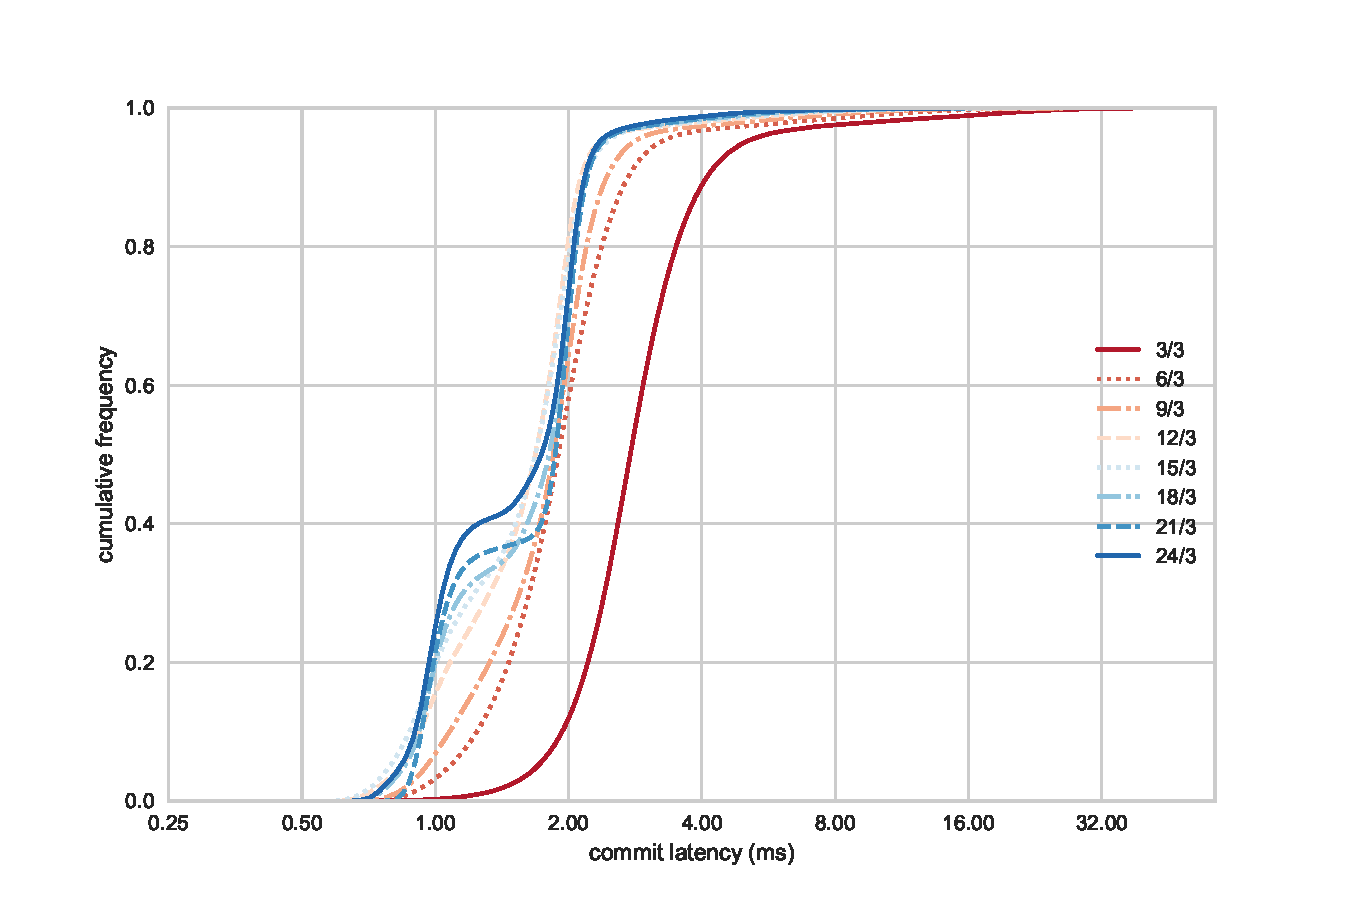
\includegraphics[width=5in]{figures/ch03_ec2_latency_cumfreq.pdf}
    \end{center}
    \renewcommand{\baselinestretch}{1}
    \small\normalsize

    \begin{quote}
        \caption[HC Cumulative Latency Distribution]{}
        \label{fig:ch03_ec2_latency_cumfreq}
    \end{quote}
\end{figure}
\renewcommand{\baselinestretch}{2}
\small\normalsize

The effect of saturation is also demonstrated in Figure~\ref{fig:ch03_ec2_latency_cumfreq}, which shows cumulative latency distributions for different system sizes holding the  workload (number of concurrent clients) constant.
The fastest (24/3) shows nearly 80\% of client write requests being serviced in under 2 msec.
Larger system sizes are faster because the smaller systems suffer from contention (25 clients can saturate a single subquorum).
Because throughput is directly related to commit latency, throughput variability can be mitigated by adding additional subquorums to balance load.

Besides pure performance and scaling, HC is also motivated by the need to adapt to varying environmental conditions.
In the next set of experiments, we explore two common runtime scenarios that motivate adaptation: shifting client workloads and failures.
We show that HC is able to adapt and recover with little loss in performance. These scenarios are shown in Figures~\ref{fig:ch03_umd_sawtooth} and \ref{fig:ch03_umd_fault_tolerance} as throughput over time, where vertical dotted lines indicate an epoch change.

\begin{figure}
    \begin{center}
        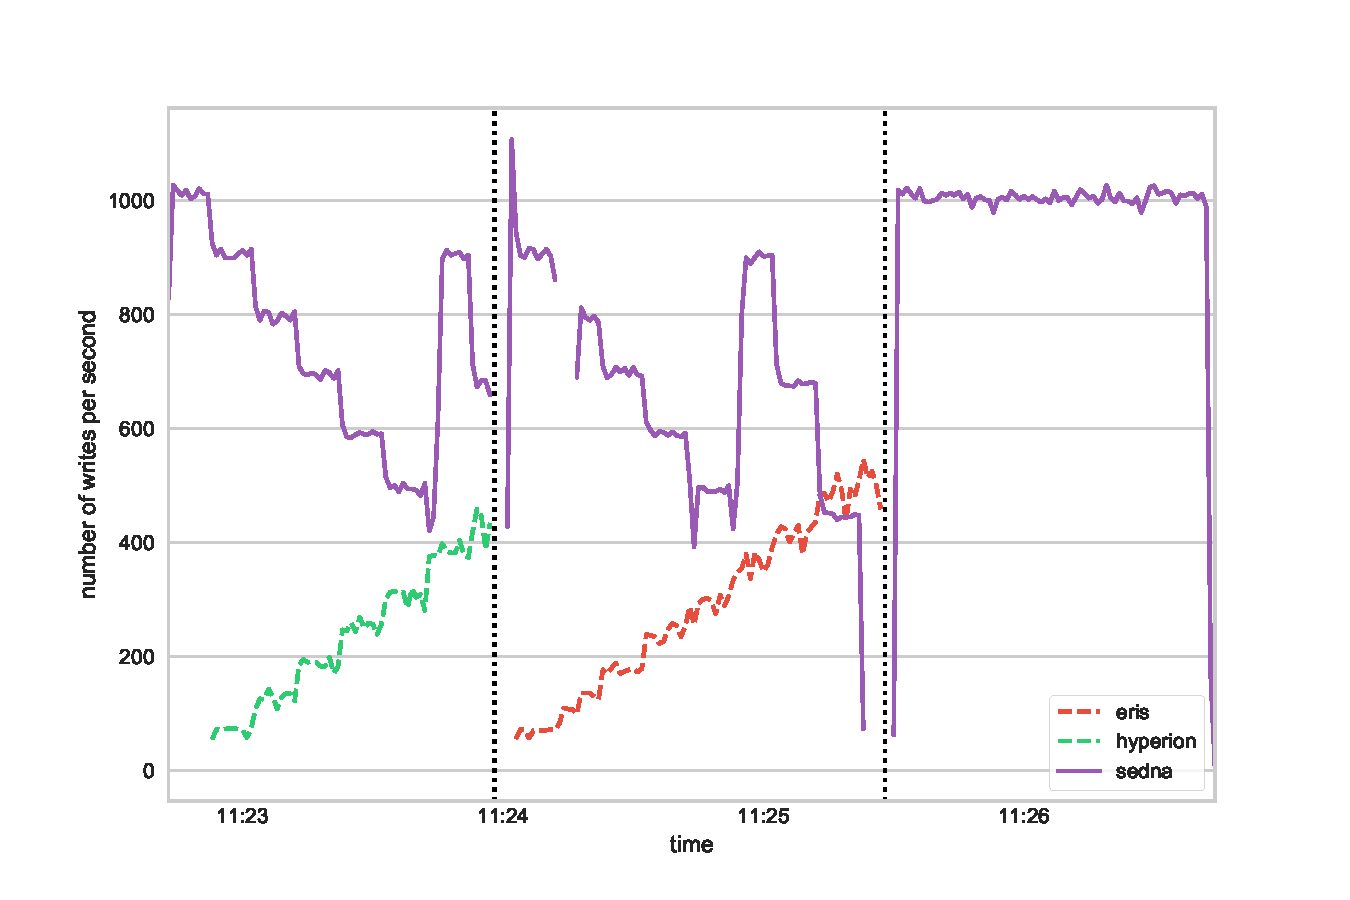
\includegraphics[width=5in]{figures/ch03_umd_sawtooth.pdf}
    \end{center}
    \renewcommand{\baselinestretch}{1}
    \small\normalsize

    \begin{quote}
        \caption[Sawtooth Graph]{9/3 system adapting to changing client access patterns by repartitioning the tag space so that clients are co-located with subquorums that serve tags they need.}
        \label{fig:ch03_umd_sawtooth}
    \end{quote}
\end{figure}
\renewcommand{\baselinestretch}{2}
\small\normalsize

The first scenario, described by the time series in Figure~\ref{fig:ch03_umd_sawtooth} shows an HC 3-replica configuration moving through two epoch changes.
Each epoch change is triggered by the need to localize tags accessed by
clients to nearby subquorums.
% The experiment was run over machines with widely varying latency.
The scenario shown starts with all clients co-located with the subquorum serving the tag they are accessing.
However, clients incrementally change their access patterns first to a tag located on one remote subquorum, and then to the tag owned by the other.
In both cases, the root quorum adapts the system by repartitioning the tagspace such that the tag defining their current focus is served by the co-located subquorum.

\begin{figure}
    \begin{center}
        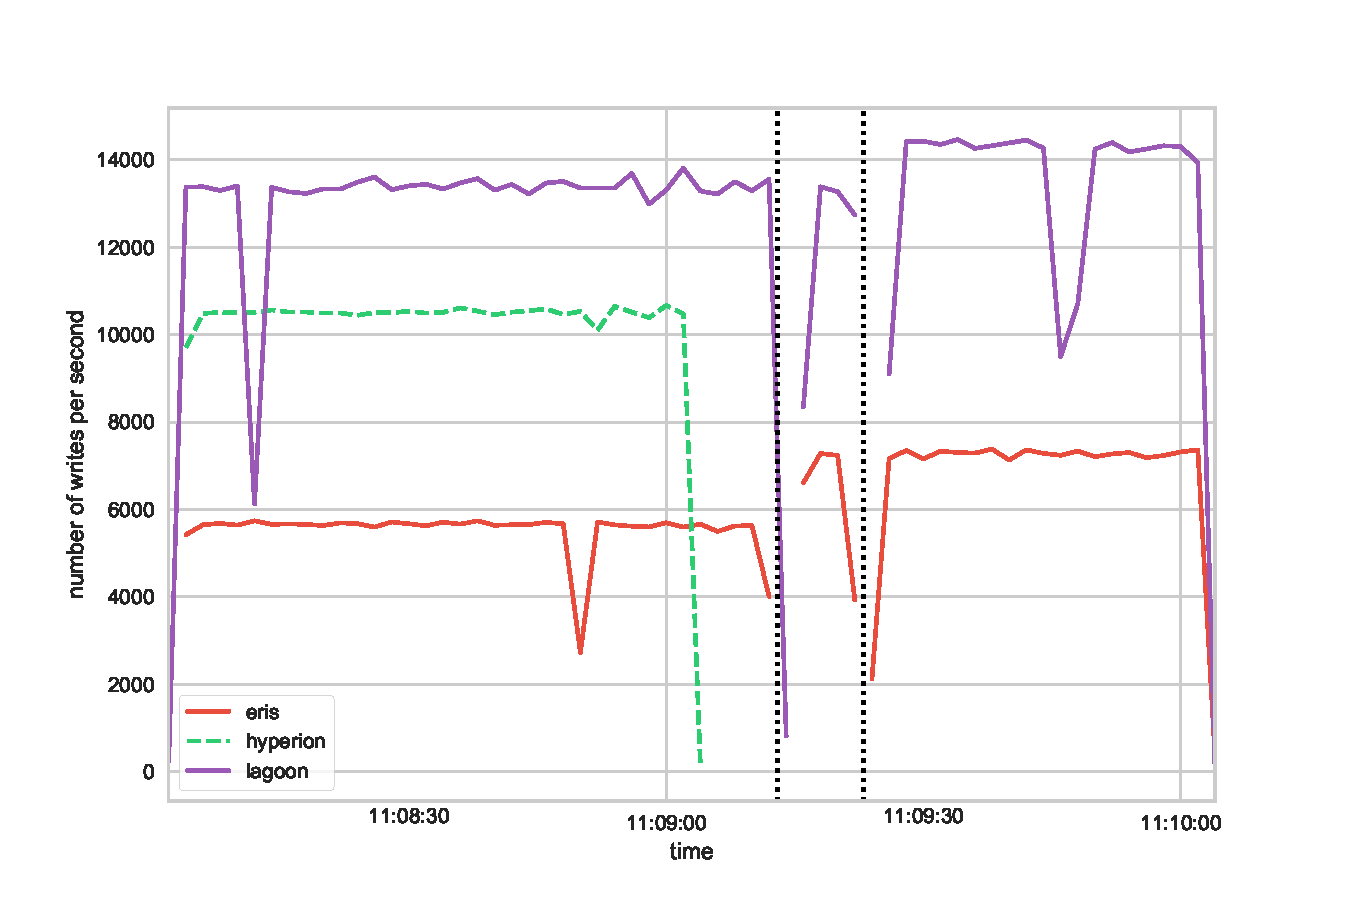
\includegraphics[width=5in]{figures/ch03_umd_fault_tolerance.pdf}
    \end{center}
    \renewcommand{\baselinestretch}{1}
    \small\normalsize

    \begin{quote}
        \caption[HC Fault Repartitioning]{9/3 System that adapts to failure (partition) of entire subquorum. After timeout, the root quorum re-partitions the tag allocated to the failed subquorum among the other two subquorums.}
        \label{fig:ch03_umd_fault_tolerance}
    \end{quote}
\end{figure}
\renewcommand{\baselinestretch}{2}
\small\normalsize

Finally, Figure~\ref{fig:ch03_umd_fault_tolerance} shows a 3-subquorum configuration where one entire subquorum becomes partitioned from the others.
After a timeout, the root uses an epoch change to re-allocate the tag of the partitioned subquorum over the two remaining subquorums.
The partitioned subquorum eventually has an \emph{obligation timeout}, after which the root quorum is not obliged to leave the tag with the current subquorum.
The tag may then be re-assigned to any other subquorum.
Timeouts are structured such that by the time an obligation timeout fires, the root quorum has already re-mapped that subquorum's tag to other subquorums.
As a result, the system is able to recover from the partition as fast as possible.
Note that in this figure, the repartition occurs through two epoch changes, the first allocating part of the tagspace to the first subquorum, and the second allocating the rest of the tag to the other.
Gaps in the graph are periods where the subquorums are electing local leaders.
This may be optimized by having leadership assigned or maintained through root consensus.

\section{Conclusion}

Most consensus algorithms have their roots in the Paxos algorithm, originally described in parliamentary terms.
The metaphor of government still applies well as we look at the evolution of distributed coordination as systems have grown to include large numbers of processes and geographies.
Systems that use a dedicated leader are easy to reason about and implement, however, like chess, if the leader goes down the system cannot make any\ progress.
Simple democracies for small groups solve this problem but do not scale, and as the system grows, it fragments into tribes.
Inspired by modern governments, we have proposed a representative system of consensus, hierarchical consensus, such that replicas elect leaders to participate in a root quorum that makes decisions about the global state of the system.
Local decision making, the kind that effects only a subset of clients and objects is handled locally by subquorums as efficiently as possible.
The result is a a hierarchy of decision making that takes advantage of hierarchies that already exist in applications.

Hierarchical Consensus is an implementation and extension of Vertical Paxos.
Like Vertical Paxos, HC reasons about consistency across all objects by identifying commands with a grid ordering (rather than a log ordering) and is reconfigurable to adapt to dynamic environments that exist in geo-replicated systems.
Adaptability allows HC to exploit locality of access, allowing for high performance coordination, even with replication across the wide area.
HC extends Vertical Paxos to ensure that intersections exist between the subquorums and the root quorum to ensure coordination exists between subquorums and to ensure that the system operates as a coordinated whole.
To scale the consensus protocol of the root quorum, we propose a novel approach, delegation, to ensure that all replicas participate in consensus but limit the number and frequency of messages required to achieve majority.
Finally, we generalized HC from primary-backup replication to describe more general online replication required by distributed databases and file systems.

In the next chapter we'll explore a hybrid consistency model implemented by federating replicas that participate in different consistency protocols.
In a planetary scale network, HC provides the strong consistency backbone of the federated model, increasing the overall consistency of the system by making coordinating decisions at a high level, and allowing high availability replicas in the fog operate independently where necessary.

%Chapter 4

\renewcommand{\thechapter}{4}

\chapter{Federated Consistency}
\label{ch:federated_consistency}
% Overview, details, consistency, performance, lessons learned.

Hybrid consistency model

\section{Overview}

\section{Eventual Consistency}

\todo{Read/Write Quorums}

Clients can \texttt{Put} (write) and \texttt{Get} (read) key-value pairs to
 and from one or more replicas in a single operation.
The set of replicas that responds to a client creates a quorum that must
agree on the state of the operation at its conclusion.
Clients can vary read and write quorum sizes to improve consistency or
availability -- larger quorums reduce the likelihood of inconsistencies
caused by concurrent updates, but smaller quorums respond much more quickly,
particularly if the replicas in the quorum are co-located with the client.
In large, geo-replicated systems we assume that clients will prefer to choose
fewer, local replicas to connect with, optimistic that collisions across the
wide-area are rare, e.g. that writes are localized but reads are global.

On \texttt{Put}, the instance of the key-value pair created by the update is
assigned a monotonically increasing, conflict-free \textit{version
number}~\cite{version_conflict_detection,version_vectors}.
For simplicity, we assume a fixed number of replicas, therefore each version
is made up of two components: the \textit{update} and \textit{precedence ids}.
Precedence ids are assigned to replicas during configuration, and update ids
are incremented to the largest observed value during synchronization.
As a result, any two versions generated by a \texttt{Put} anywhere in the
system are comparable such that the \textit{latest} version of the key-value
pair is the version with the largest update id, and in the case of ties, the
largest precedence id.

Additional version metadata, including the parent version of the update (in a
read-then-write system or simply the latest version of the key stored
locally), implements a virtual object history that allows us to reason about
consistency.
Keys can be managed independently, e.g. each key has its own update id
sequence resulting in per-object consistency, or all objects can be managed
together with a single sequence; in the latter case, it is possible to
construct an ordering history of operations to all objects and in the former,
a sequence of operations for each object.
Object histories allow us to reason about the global consistency of the
system.

There are two primary inconsistencies that can occur in this system:
\textit{stale reads} and \textit{forked writes}.
A stale read means that the \texttt{Get} operation has not returned
the globally most recent version of the object, e.g. the local replica is
behind in the object history.
A forked write is caused when there are two concurrent writes to the same
object, a symptom of stale reads.
Forked writes cause a divergence in the object history such that there are
two or more branches of update operations.
As we will see in the next section, one of these writes will eventually be
\textit{stomped} before it can become fully replicated, meaning that the
eventual consistency prunes these branches at the cost of losing
the update.
The ideal consistency for a system is represented by a linear object history
without forks~\cite{rethinking_eventual}, which demonstrates that the
system was in a consistent state during all accesses.

% In chapter 6
% Both forms of inconsistency can be primarily attributed to \emph{visibility
% latency}, that is the time it takes for an update to propagate to all
% replicas in the system.
% Visibility latency is directly related to the likelihood of stale reads with
% respect to the frequency of accesses~\cite{quantifying_pbs}; said
% another way, decreasing the visibility latency improves the overall
% consistency of a system.
% However, in a system that uses anti-entropy for replication, the propagation
% speed of an update is not governed solely by network connections, it is also
% bound to the number and frequency of anti-entropy sessions conducted as well
% as the radius of the network.

\todo{Anti-Entropy Sessions and Synchronization}

Anti-entropy sessions are conducted in a pairwise fashion on a periodic
interval to ensure that the network is not saturated with synchronization
requests which may reduce client availability.
At each interval, every replica selects a synchronization partner such that
all replicas have a uniform likelihood of selection.
This ensures that an update originating at one replica will be propagated to
all online replicas given the continued operation of replication.
This mechanism also provides robustness in the face of failure; a single
unresponsive replica or even network partition does not become a bottleneck
to synchronization, and once the failure is repaired synchronization will
occur without reconfiguration.

There are two basic forms of synchronization: \textit{push} synchronization
is a fire-and-forget form of synchronization where the remote replica is sent
the latest version of all objects, whereas \textit{pull} synchronization
requests the latest version of objects and minimizes the size of data
transfer.
To get the benefit of both, we consider \textit{bilateral} synchronization
which combines push and pull in a two-phase exchange.
Bilateral synchronization increases the effect of anti-entropy during each
exchange because it ensures that in the common case each replica is
synchronized with two other replicas instead of one during every anti-entropy
period.

Bilateral anti-entropy starts with the initiating replica sending a vector of
the latest local versions of all keys currently stored, usually optimized
with Merkel or prefix trees to make comparisons faster.
The remote replica compares the versions sent by the initiating replica with
its current state and responds with any objects whose version is
\textit{later} than the initiating replica's as well as another version
vector of requested objects that are earlier on the remote.
The initiating replica then replies with the remote's requested objects,
completing the synchronization.
We refer to the first stage of requesting later objects from the remote as
the pull phase, and the second stage of responding to the remote the push
phase.

There are two important things to note about this form of anti-entropy
exchange.
First, this type of synchronization implements a \textit{latest writer wins}
policy.
This means that not all versions are guaranteed to become fully replicated
-- if a later version is written during propagation of an earlier version,
then the earlier version gets \emph{stomped} by the later version because
only the latest versions of objects are exchanged.
If there are two concurrent writes, only one write will become fully
replicated, the write on the replica with the greater precedence.

% IN Chapter 6 
% Second, visibility latency is maximized when all replicas choose a remote
% synchronization partner that does not yet have the update.
% This means that maximal visibility latency is equal to $t\log_3n$, where
% $t$ is the anti-entropy interval and $n$ is the number of replicas in the
% network.
% In practice, however, because of inefficient exchanges due to uniform random
% selection of synchronization partners, this latency is never practically
% achieved, and is instead modulated by a noise variable that is
% proportional to the size of the network.

Policies: latest writer wins

Bilateral anti-entropy

\subsection{Consistency Failures}

Forks

Stale Reads

\section{Integration}

\subsection{Communication Integration}

\subsection{Consistency Integration}

- Forte Number

\section{Performance Evaluation}

Communication Topology
Inconsistencies due to outages
Inconsistency due to system latency

%Chapter 5

\renewcommand{\thechapter}{5}

%TODO: Add better title
\chapter{System Implementation}

Given its grandiose title, it may seem that the engineering behind the development of a planetary scale data storage system would require thousands of man-hours of professional software engineers and a highly structured development process.
In fact, this is not necessarily the case for two reasons.
First, data systems benefit from an existing global network topology and commercial frameworks for deploying applications.
This means that both the foundation and motivation for creating large geo-replicated systems exists, as described earlier.
Second, like the internet, complex global systems emerge through the composition of many simpler components following straight forward rules~\cite{internet}.
Instead of architecting a monolithic system, the design process is decomposed to reasoning about the behavior of single processes.
Rather than being built, a robust planetary data system evolves from its network environment.

To facilitate system evolution, the consistency models we have described thus far have been \emph{composable} to allow heterogeneous replicas to participate in the same system.
However, while composability allows us to reason about consistency expectations, it does not necessarily mean interoperability.
In order to ensure reason about system expectations we must outline our assumptions for communication, security, processing, and data storage.
In this chapter, we describe the implementation of the replicas and applications of our experimental system and the assumptions we made.

%TODO: make this opening section better when we figure out where it fits.

\section{System Model}

A \emph{replica} is an independent process that maintains a portion of the objects stored as well as a \emph{view} of the state of the entire system.
Replicas must be able to communicate with one another and may also \emph{serve} requests from clients.
A system is composed of multiple communicating replicas and is defined by the behavior the replicas.
For example, a totally replicated system is one where each replica stores a complete copy of all objects as in the primary-backup approach~\cite{primary_backup}, whereas a partially replicated system ensures durability such that multiple replicas store the same object but not all replicas store all objects as in the Google File System~\cite{gfs}.
At the scale of a multi-region, globally deployed system, we assume that total replication is impractical and primarily consider the partial replication case.

Let's unpack some of the assumptions made by the seemingly simple statements made in the previous paragraph.
First, independence means replicas have a shared-nothing architecture~\cite{shared_nothing} and cannot share either memory or disk space.
For practical purposes of fault tolerance, we generally assume that there is a one-to-one relationship between a replica and a disk so that a disk failure means only a single replica failure.
Second, that each replica must maintain a view of the state of the entire system means both that replicas must be aware of their peers on the network and that they should know the locations of objects stored on the network.
A strict interpretation of this requirement would necessarily make system membership brittle as it would be difficult to add or remove replicas.
Alternatively, a centralized interpretation of the view requirement would allow for


Second, the ability to communicate with replicas and serve requests from clients means that the replica must be addressable.


This requirement is seemingly innocuous when taken by itself, however when we also describe a replica as requiring a view of the state of the entire system, it means that a replica must know about the existence of all other replicas in the system.
A strict interpretation of having a complete view would necessarily make the system composition brittle, unable to add or remove replicas.
Instead we take a less strict view


- networking
- actors
- event loop
- reasons why the above are important
-

\section{Applications}

\subsection{Distributed Log}

\subsection{Key-Value Database}

\subsection{File System}

\section{Consistency Model}

Client-side vs. system-side consistency

Log model of consistency

Continuous consistency scale

Grid consistency model


\section{Conclusion}

We did not optimize our research for the minimum set of assumptions required to facilitate interoperability between heterogeneous replicas.
However, we hope that the assumptions we did make shed light on what is required to achieve the minimum set of assumptions.

Further research is required to ...

%Chapter 6

\renewcommand{\thechapter}{6}

\chapter{Adaptive Consistency}
\label{ch:adaptive_consistency}

Throughout this dissertation we have outlined a planetary-scale data storage system composed of a two-tier structure that provides a hybrid consistency model.
Both tiers are designed to scale to thousands of replicas, and together could represent millions of replicas operating in concert around the world.
Management and systems administration of such a large scale system using external monitoring processes is impractical at best and prohibitively complex at worst.
Even with a trusted infrastructure of cloud services, building a single synchronization point for monitoring and optimization would require the online collection of live information from across the globe.
This synchronization point would itself be susceptible to delays and partitions and would have to manage a huge number of events streaming in from many sources, which has challenges in and of itself~\cite{spark_streaming}.

Instead, we propose that an \emph{emergent model} of network behavior is required to tune and optimize planetary scale systems at runtime such that local, simple rules lead to globally emergent behavior~\cite{bengfort_evolutionary_2014}.
Specifically we hypothesize that when individual replicas follow simple optimization procedures based on monitoring of their local network performance, access patterns, queries to their neighbors, and other environmental factors the performance of the system will collectively increase.
Because we focus primarily on the consistency aspects of geo-replicated data storage, we have termed this behavior \emph{adaptive consistency}, because with a hybrid or continuous consistency model, such optimizations will minimize inconsistent behaviors due to latency or configuration.

In this chapter we will show we can improve consistency of the system as a whole with localized machine learning implemented on a per-replica basis.
Although this work is largely left for future research on a fully deployed platform, we have built our system with this kind of adaptation in mind.
Our preliminary experiments suggest that adapting anti-entropy selection with reinforcement learning techniques will meaningfully enhance consistency in the federated fog layer of the system~\cite{bengfort_anti-entropy_2018}.
We will then finish with a discussion of how we can generalize this process to other techniques in the system as a whole.

\section{Anti-Entropy Bandits}
\label{ch06_anti_entropy_bandits}

A distributed system is made highly available when individual servers are
allowed to operate independently without failure-prone, high latency
coordination.
The independent nature of the server's behavior means that it can immediately
respond to client requests, but that it does so from a limited, local
perspective which may be inconsistent with another server's response.
If individual servers in a system were allowed to remain wholly independent,
individual requests from clients to different servers would create a lack of
order or predictability, a gradual decline into inconsistency, i.e. the
system would experience \textit{entropy}.
To combat the effect of entropy while still remaining highly available,
servers engage in periodic background \textit{anti-entropy
  sessions}~\cite{bayou}.

Anti-entropy sessions synchronize the state between servers ensuring that,
at least briefly, the local state is consistent with a portion of the global
state of the system.
If all servers engage in anti-entropy sessions, the system is able to make
some reasonable guarantees about consistent replication; the most well known
of which is that without requests the system will become
globally consistent, eventually~\cite{anti_entropy}.
More specifically, inconsistencies in the form of stale reads can be bound by
likelihoods that are informed by the latency of anti-entropy sessions and the
size of the system~\cite{probabilistically_bounded_staleness,quantifying_pbs}.
Said another way, overall consistency is improved in an eventually consistent
system by decreasing the likelihood of a stale read, which is tuned by
improving the \textit{visibility latency} of a write, the speed at which a
write is propagated to a significant portion of servers.
This idea has led many system designers to decide that eventual consistency
is ``consistent enough''~\cite{bermbach_eventual_2011,wada_data_2011},
particularly in a data center context where visibility latency is far below
the rate of client requests, leading to practically strong consistency.

However, propagation rates need to be re-evaluated when replicas move outside of data center contexts and when anti-entropy is replicating across the wide area.
Our system envisions a \emph{fog layer} that provides data services to localized regions with a hybrid consistency model.
The fog is specifically designed to handle mobile users, sensor systems, and high throughput applications at the edge of the data center backbone~\cite{edge_computing,geo_cdn}.
However, scaling an eventually consistent system to dozens or even hundreds
of nodes increases the radius of the network, which leads to increased noise
during anti-entropy e.g. the possibility that an anti-entropy session will be
between two already synchronized nodes.
Geographic distribution and extra-datacenter networks also increase the
latency of anti-entropy sessions so that inconsistencies become more apparent
to external observers.

To address this challenge, we propose the use of reinforcement learning techniques to optimize network behavior by minimizing latency.
Anti-entropy uses gossip and rumor spreading to propagate updates
deterministically without saturating the
network even in the face of network
outages~\cite{gossip_protocols,rumor_spreading,rumor_spreading_dynamics}.
These protocols use uniform random selection to choose synchronization peers,
which means that a write occurring at one replica is not efficiently
propagated across the network.
In this section we explore the use of \textit{multi-armed bandit}
algorithms~\cite{epoch_greedy_mab,contextual_bandits} to optimize
for fast, successful synchronizations by modifying peer selection
probabilities.
The result is a synchronization topology that emerges according to access
patterns and network latencies.
As we will show in the next sections, such topologies produce efficient synchronization,
localize most data exchanges, lower visibility latency, and increase
consistency.

\subsection{Visibility Latency}
\label{ch06_visbility}

In this section we review the access and consistency model in the context of bandits as well as how anti-entropy is conducted.
A more complete discussion of these topics can be found in Chapter~\ref{ch:federated_consistency}.

Clients can \texttt{Put} (write) and \texttt{Get} (read) key-value pairs to
and from one or more replicas in a single operation, creating read and write quorums that improve consistency by enforcing coordination between replicas on the access.
In large, geo-replicated systems, we assume that clients prefer to choose fewer, local replicas to connect with, assuming that writes are primarily local and reads are global.
On \texttt{Put}, a new conflict-free version of the write is created.
This results in the possibility of two types of inconsistencies that occur during concurrent accesses: stale reads and forked writes.
As a write is propagated through the system, the latest-writer wins policy means that at least one of the forks will be ``stomped,'' e.g. not fully replicated.

Both forms of inconsistency can be primarily attributed to \emph{visibility
latency}, that is the time it takes for an update to propagate to all
replicas in the system.
Visibility latency is directly related to the likelihood of stale reads with
respect to the frequency of accesses~\cite{quantifying_pbs}; said
another way, decreasing the visibility latency improves the overall
consistency of a system.
However, in a system that uses anti-entropy for replication, the propagation
speed of an update is not governed solely by network connections, it is also
bound to the number and frequency of anti-entropy sessions conducted as well
as the radius of the network.

Visibility latency is minimized when all replicas choose a remote
synchronization partner that does not yet have the update.
This means that minimal visibility latency is equal to $t\log_3n$, where
$t$ is the anti-entropy interval and $n$ is the number of replicas in the
network.
In practice, however, because of inefficient exchanges due to uniform random
selection of synchronization partners, this latency is never practically
achieved, and is instead modulated by a noise variable that is
proportional to the size of the network.

\subsection{Multi-Armed Bandits}
\label{ch06_multi_armed_bandits}

To combat the effect of noise on visibility latency our initial approach
employs a technique commonly used in active and reinforcement learning:
multi-armed bandits.
Multi-armed bandits refer to a statistical optimization procedure that is
designed to find the optimal payout of several choices that each have
different probabilities of reward.
In this case, we use bandits to improve uniform random selection of peers so
that replicas choose synchronization partners that are most likely to exchange
information, and thus more quickly propagate updates, while still maintaining
the properties of full replication and fault tolerance.

A bandit problem is designed by identifying several (usually more than two)
competing choices called ``arms''\renewcommand{\baselinestretch}{1} \small\footnotesize\footnote{Arms refer to the pulling
mechanism of a slot machine, the metaphor generally used to motivate the
multi-armed bandit problem.}\renewcommand{\baselinestretch}{2} \small\normalsize, as well as a reward function that determines how
successful the selection of an arm is.
During operation, the bandit selects an arm, observes the rewards, then
updates the payout likelihood of the selected arm, normalized by the number
of selections.
As the bandit selects arms, it learns which arm or arms have the highest
likelihood of reward, and can modify it's arm selection \emph{strategy} to
maximize the total reward over time.

Bandits must balance exploration of new arms with possibly better reward
values and exploitation of an arm that has higher rewards than others.
In an \emph{epsilon greedy strategy}, the bandit will select the arm with
the best reward with some probability $1-\epsilon$, otherwise it will select
any of the arms with uniform probability.
The smaller $\epsilon$ is, the more the bandit favors exploitation of known
good arms, the larger $\epsilon$ is, the more it favors exploration.
If $\epsilon=1$ then the algorithm is simply uniform random selection.
A simple extension of this is a strategy called \emph{annealing epsilon
greedy}, which starts with a large $\epsilon$, then as the number of trials
increases, steadily decreases $\epsilon$ on a logarithmic scale.
There are many other bandit strategies but we have chosen these two simple
strategies for our initial research to demonstrate a bolt-on effective
improvement to existing systems.

Peer selection for anti-entropy is usually conducted with uniform random
selection to guarantee complete replication.
To extend anti-entropy with bandits, we design a selection method whose arms
are remote peers and whose rewards are determined by the success of
synchronization.
The goal of adding bandits to anti-entropy is to optimize selection of peers
such that the visibility latency becomes closer to the optimal propagation
time as a synchronization topology emerges from the bandits.
A secondary goal is to minimize anti-entropy latency by preferring local (in
the same data center) and regional (e.g. on the same continent) connections.

Our initial reward function favors synchronizations to replicas where the
most writes are occurring by giving higher rewards to anti-entropy sessions
that exchange later versions in either a push or a pull, as well as additional
rewards if more than one object is exchanged.
Additionally, the latency of the synchronization RPCs is computed to reward
replicas that are near each other.
The complete reward function is given in Table~\ref{tab:ch06_rewards}: for each
phase of synchronization (push and pull), compute the reward as the sum of the
propositions given.
For example if a synchronization results in three objects being pulled in
250 ms, and one object being pushed in 250 ms, the reward is 0.75.

\renewcommand{\baselinestretch}{1}
\small\normalsize
 \begin{table}[t!]
\caption[Bandit Reward Function]{The rewards function for our initial anti-entropy bandits. Rewards are computed by introspecting the results of the pull and push phases of bilateral anti-entropy.}
\begin{center}
\begin{tabular}{@{}l c c c @{}}
\hline
& \textbf{Pull} & \textbf{Push} & \textbf{Total} \\
\hline \hline
Synchronize at least 1 object & 0.25 & 0.25 & 0.50 \\
Additional for multiple objects  & 0.05 & 0.05 & 0.10 \\
Latency $\leq$ 5 ms (local)        & 0.10 & 0.10 & 0.20 \\
Latency $\leq$ 100 ms (regional)   & 0.10 & 0.10 & 0.20 \\
\hline
\textit{Total} & \textit{0.50} & \textit{0.50} & \textit{1.00} \\
\hline
\end{tabular}
\end{center}
\label{tab:ch06_rewards}
\end{table}
 \renewcommand{\baselinestretch}{2}
\small\normalsize

The design of reward functions can be implemented to the needs of a specific
system.
For example, in a system that has workloads with variable sized writes, object
size could be considered or systems with imbalanced deployments might
consider a reward function that prioritizes inter-region communication.

\subsection{Experiments}
\label{ch06_experiments}

We conducted experiments using a distributed key-value store totally
replicated across 45 replicas in 15 geographic regions on 5 continents
around the world.
Replicas were hosted using AWS EC2 t2.micro instances and were connected to
each other via internal VPCs when in the same region, using external
connections between regions.
The store, called Honu, is implemented in Go 1.9 using gRPC and protocol
buffers for RPC requests; all code is open source and available on GitHub.

The workload on the system was generated by 15 clients, one in each region and
colocated with one of the replicas.
Clients continuously created Put requests for random keys with a unique
prefix per-region such that consistency conflicts only occur within a
single region.
The average throughput generated per-client was 5620.4 puts/second.
The mean synchronization latency between each region ranged from 35 ms to
630 ms as shown in Figures~\ref{fig:ch06_latency_sync_heatmap} and \ref{fig:ch06_push_pull_frankfurt_latencies}.
To ensure at least one synchronization per anti-entropy session, we set the
anti-entropy interval to 1 second to train the system, then reduced the
interval to 125 ms while measuring visibility latency.
To account for lag between commands sent to replicas in different regions,
each experiment was run for 11 minutes, the bandit learning period was 4
minutes then visibility latency was observed for 6 minutes, buffered by 30
seconds before and after the workload to allow replicas to initialize and
gracefully shutdown.

\begin{figure}
    \begin{center}
        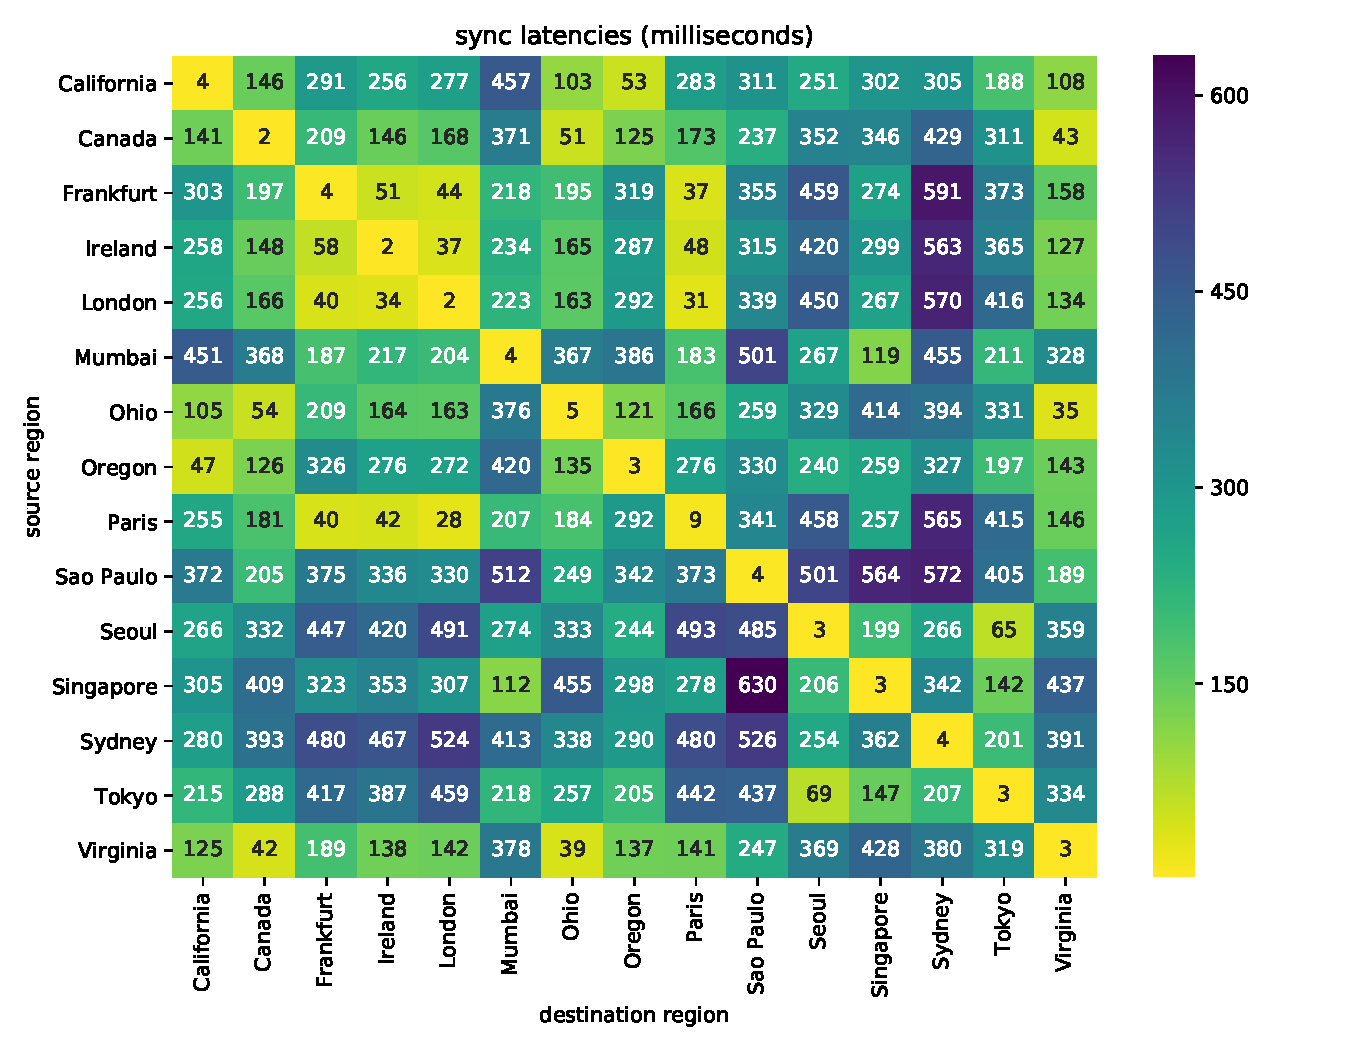
\includegraphics[width=5in]{figures/ch06_latency_sync_heatmap.pdf}
    \end{center}
    \renewcommand{\baselinestretch}{1}
    \small\normalsize

    \begin{quote}
        \caption[Anti-Entropy Synchronization Latencies]{Inter-Region Synchronization Latencies (Push+Pull)}
        \label{fig:ch06_latency_sync_heatmap}
    \end{quote}
\end{figure}
\renewcommand{\baselinestretch}{2}
\small\normalsize

\begin{figure}
    \begin{center}
        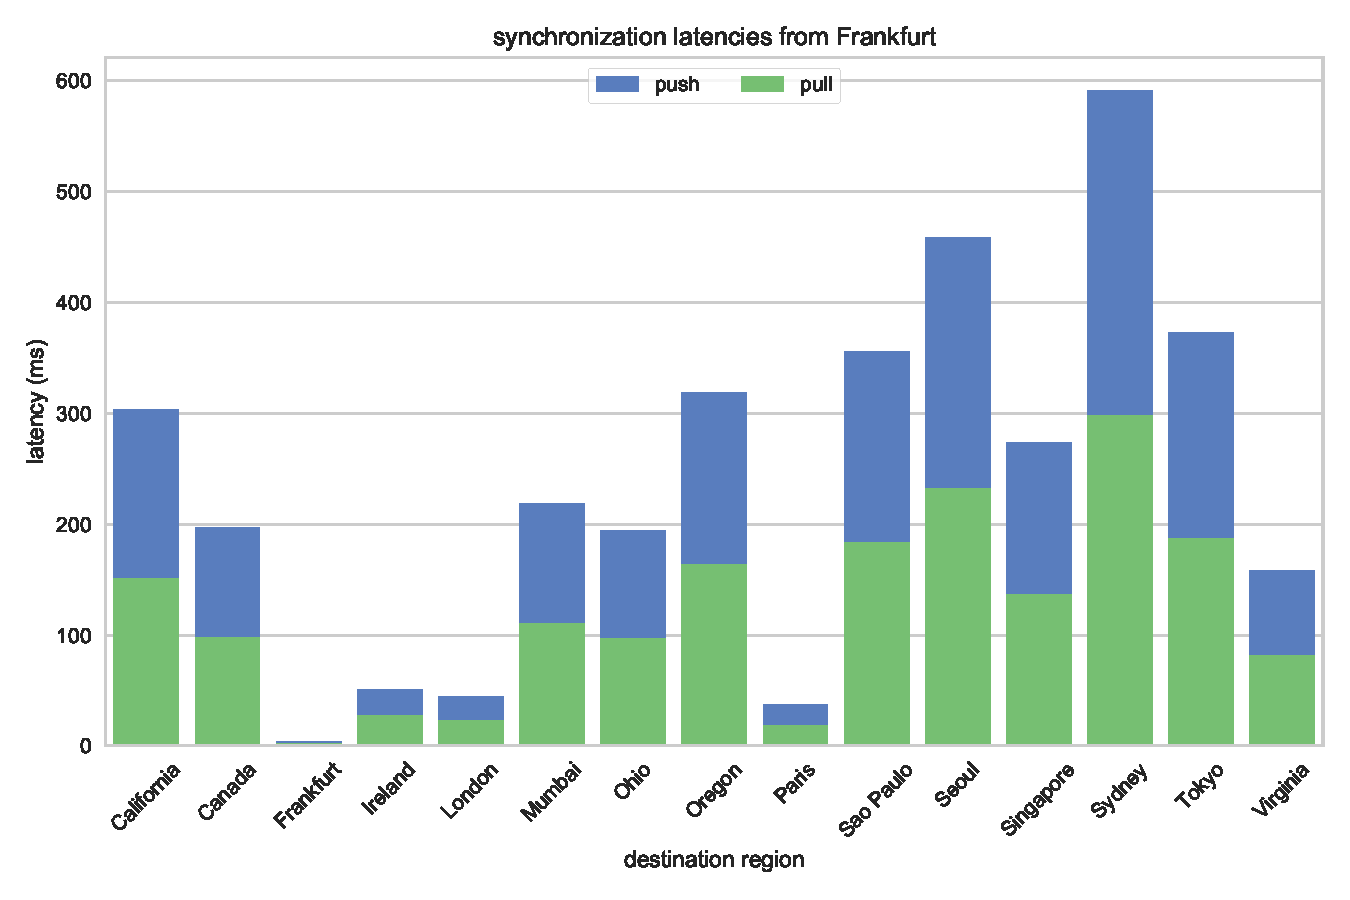
\includegraphics[width=5in]{figures/ch06_push_pull_frankfurt_latencies.pdf}
    \end{center}
    \renewcommand{\baselinestretch}{1}
    \small\normalsize

    \begin{quote}
        \caption[Anti-Entropy Synchronization Latency from Frankfurt]{View of anti-entropy synchronization latency from Europe and corresponding network distances.}
        \label{fig:ch06_push_pull_frankfurt_latencies}
    \end{quote}
\end{figure}
\renewcommand{\baselinestretch}{2}
\small\normalsize

Our first experiments compared uniform random peer selection with epsilon
greedy bandits using $\epsilon \in \{0.1, 0.2, 0.5\}$ as well as an annealing
epsilon greedy bandit.
The total system rewards as a rolling mean over a time window of 20
synchronizations are shown in Figure~\ref{fig:ch06_rewards}.
The rewards ramp up from zero as the clients come online and start
creating work to be synchronized.
All of the bandit algorithms eventually improve over the baseline of uniform
selection, not only generating more total reward across the system, but also
introducing less variability in rewards over time.
None of the bandit curves immediately produces high rewards as they explore
the reward space; lower $\epsilon$ values may cause exploitation of incorrect
arms, while higher $\epsilon$ values take longer to find optimal topologies.
However, in the static workload case, the more aggressive bandit strategies
converge more quickly to the optimal reward.

Visibility latencies were computed by reducing the workload rate to once
every 4 seconds to ensure the write becomes fully visible across the entire
network.
During the visibility measurement period, replicas locally logged the
timestamp the write was pushed or pulled; visibility latency is computed as
the difference between the minimum and maximum timestamp.
The average visibility latency per region is shown in
Figure~\ref{fig:ch06_visibility_latency} measured by the left y-axis.
Because the anti-entropy delay is a fixed interval, the estimated number of
required anti-entropy sessions associated with the visibility delay is shown
on the right y-axis of the same figure.
Employing bandit strategies reduces the visibility latency from 2360 ms on
average in the uniform case to 1870 ms, reducing the number of required
anti-entropy intervals by approximately 4.

\begin{figure}
    \begin{center}
        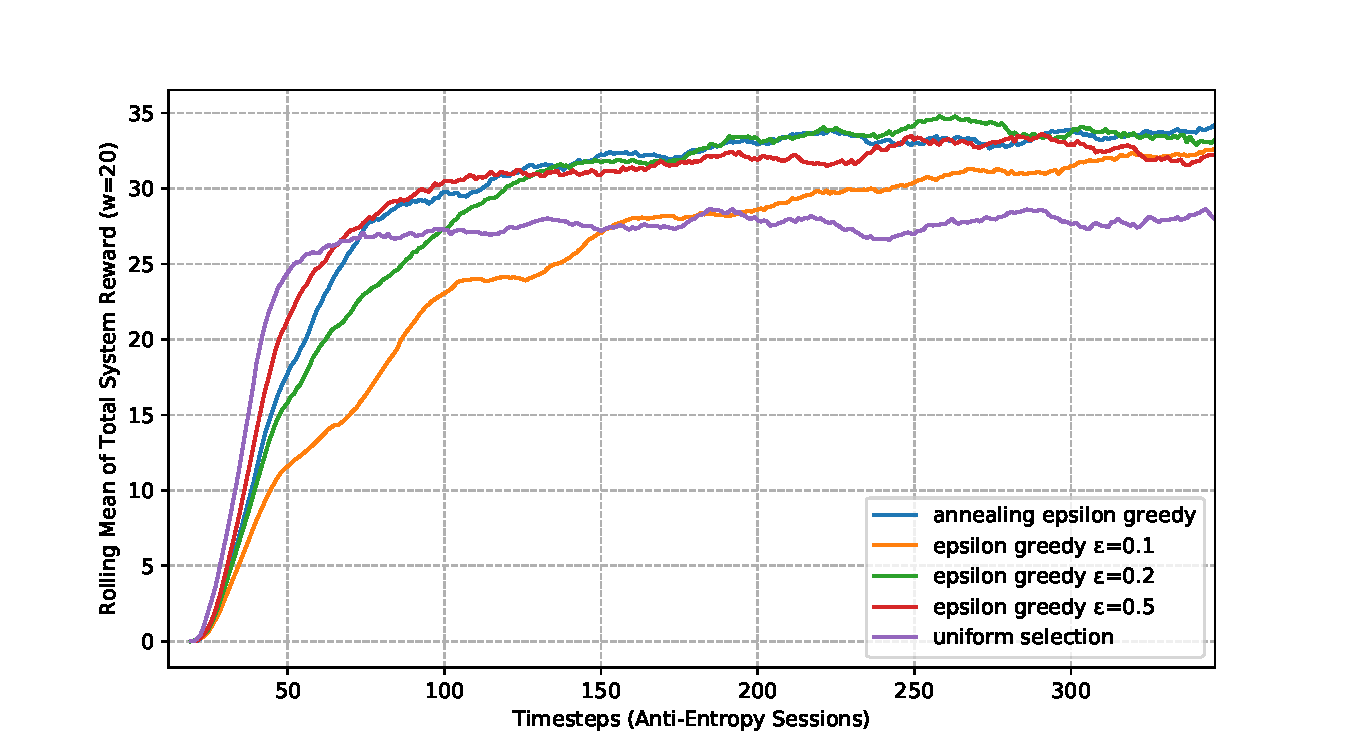
\includegraphics[width=5in]{figures/ch06_rewards.pdf}
    \end{center}
    \renewcommand{\baselinestretch}{1}
    \small\normalsize

    \begin{quote}
        \caption[Bandit Rewards]{Total system rewards over time.}
        \label{fig:ch06_rewards}
    \end{quote}
\end{figure}
\renewcommand{\baselinestretch}{2}
\small\normalsize

\begin{figure}
    \begin{center}
        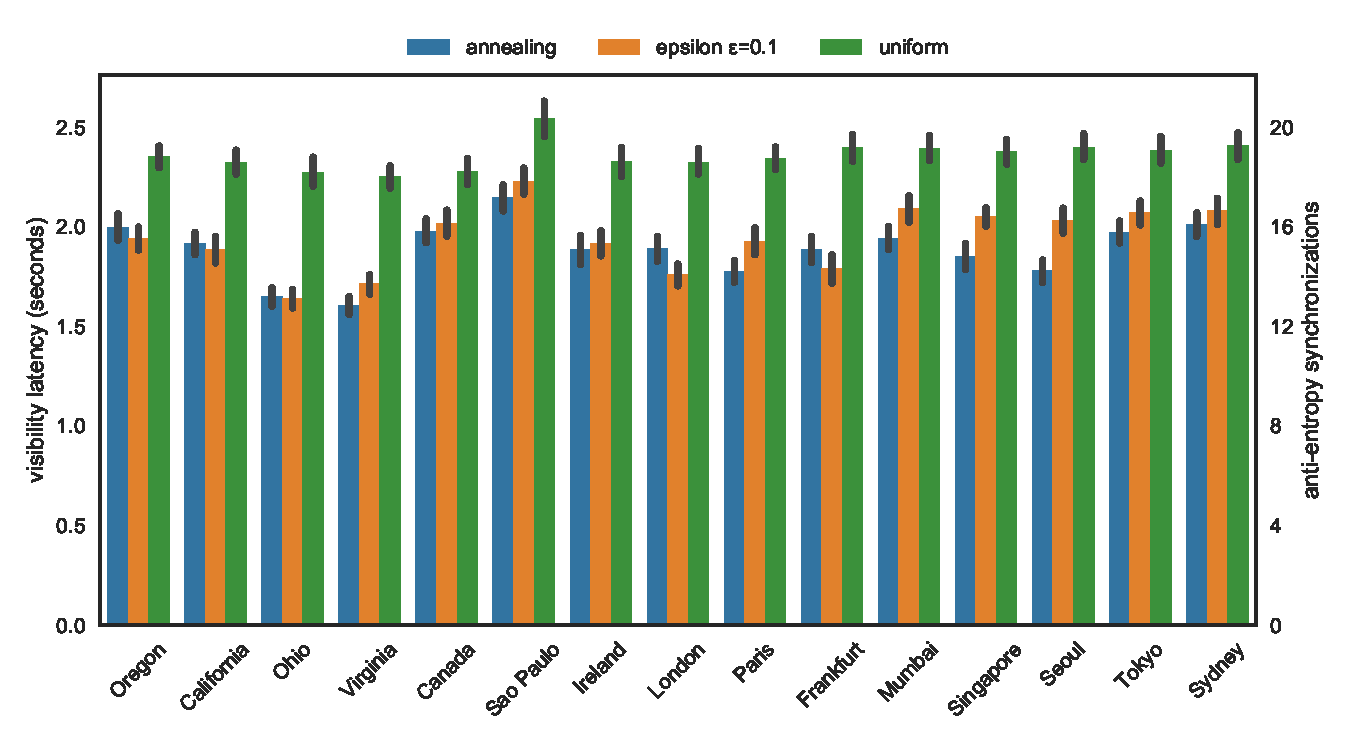
\includegraphics[width=5in]{figures/ch06_visibility_latency.pdf}
    \end{center}
    \renewcommand{\baselinestretch}{1}
    \small\normalsize

    \begin{quote}
        \caption[Visibility Latency]{Decreasing visibility latency from bandit approaches.}
        \label{fig:ch06_visibility_latency}
    \end{quote}
\end{figure}
\renewcommand{\baselinestretch}{2}
\small\normalsize

To show the emergent behavior of bandits, we have visualized the resulting
topologies as network diagrams in Figure~\ref{fig:ch06_uniform_selection_topology} (uniform
selection), Figure~\ref{fig:ch06_annealing_epsilon_toplogy} (annealing epsilon) and
Figure~\ref{fig:ch06_epsilon_greedy_topology} (epsilon greedy $\epsilon=0.2$).
Each network diagram shows each replica as a vertex, colored by region e.g.
purple is California, teal is Sao Paulo, Brazil, etc.
Each vertex is also labeled with the 2-character UN country or US state
abbreviation as well as the replica's precedence id.
The size of the vertex represents the number of \texttt{Put} requests that
replica received over the course of the experiment; larger vertices
represent replicas that were colocated with workload generators.
Each edge between vertices represents the total number of successful
synchronizations, the darker and thicker the edge is, the more
synchronizations occurred between the two replicas.
Edges are directed; the source of the edge is the replica that initiated
anti-entropy with the target of the edge.

\begin{figure}
    \begin{center}
        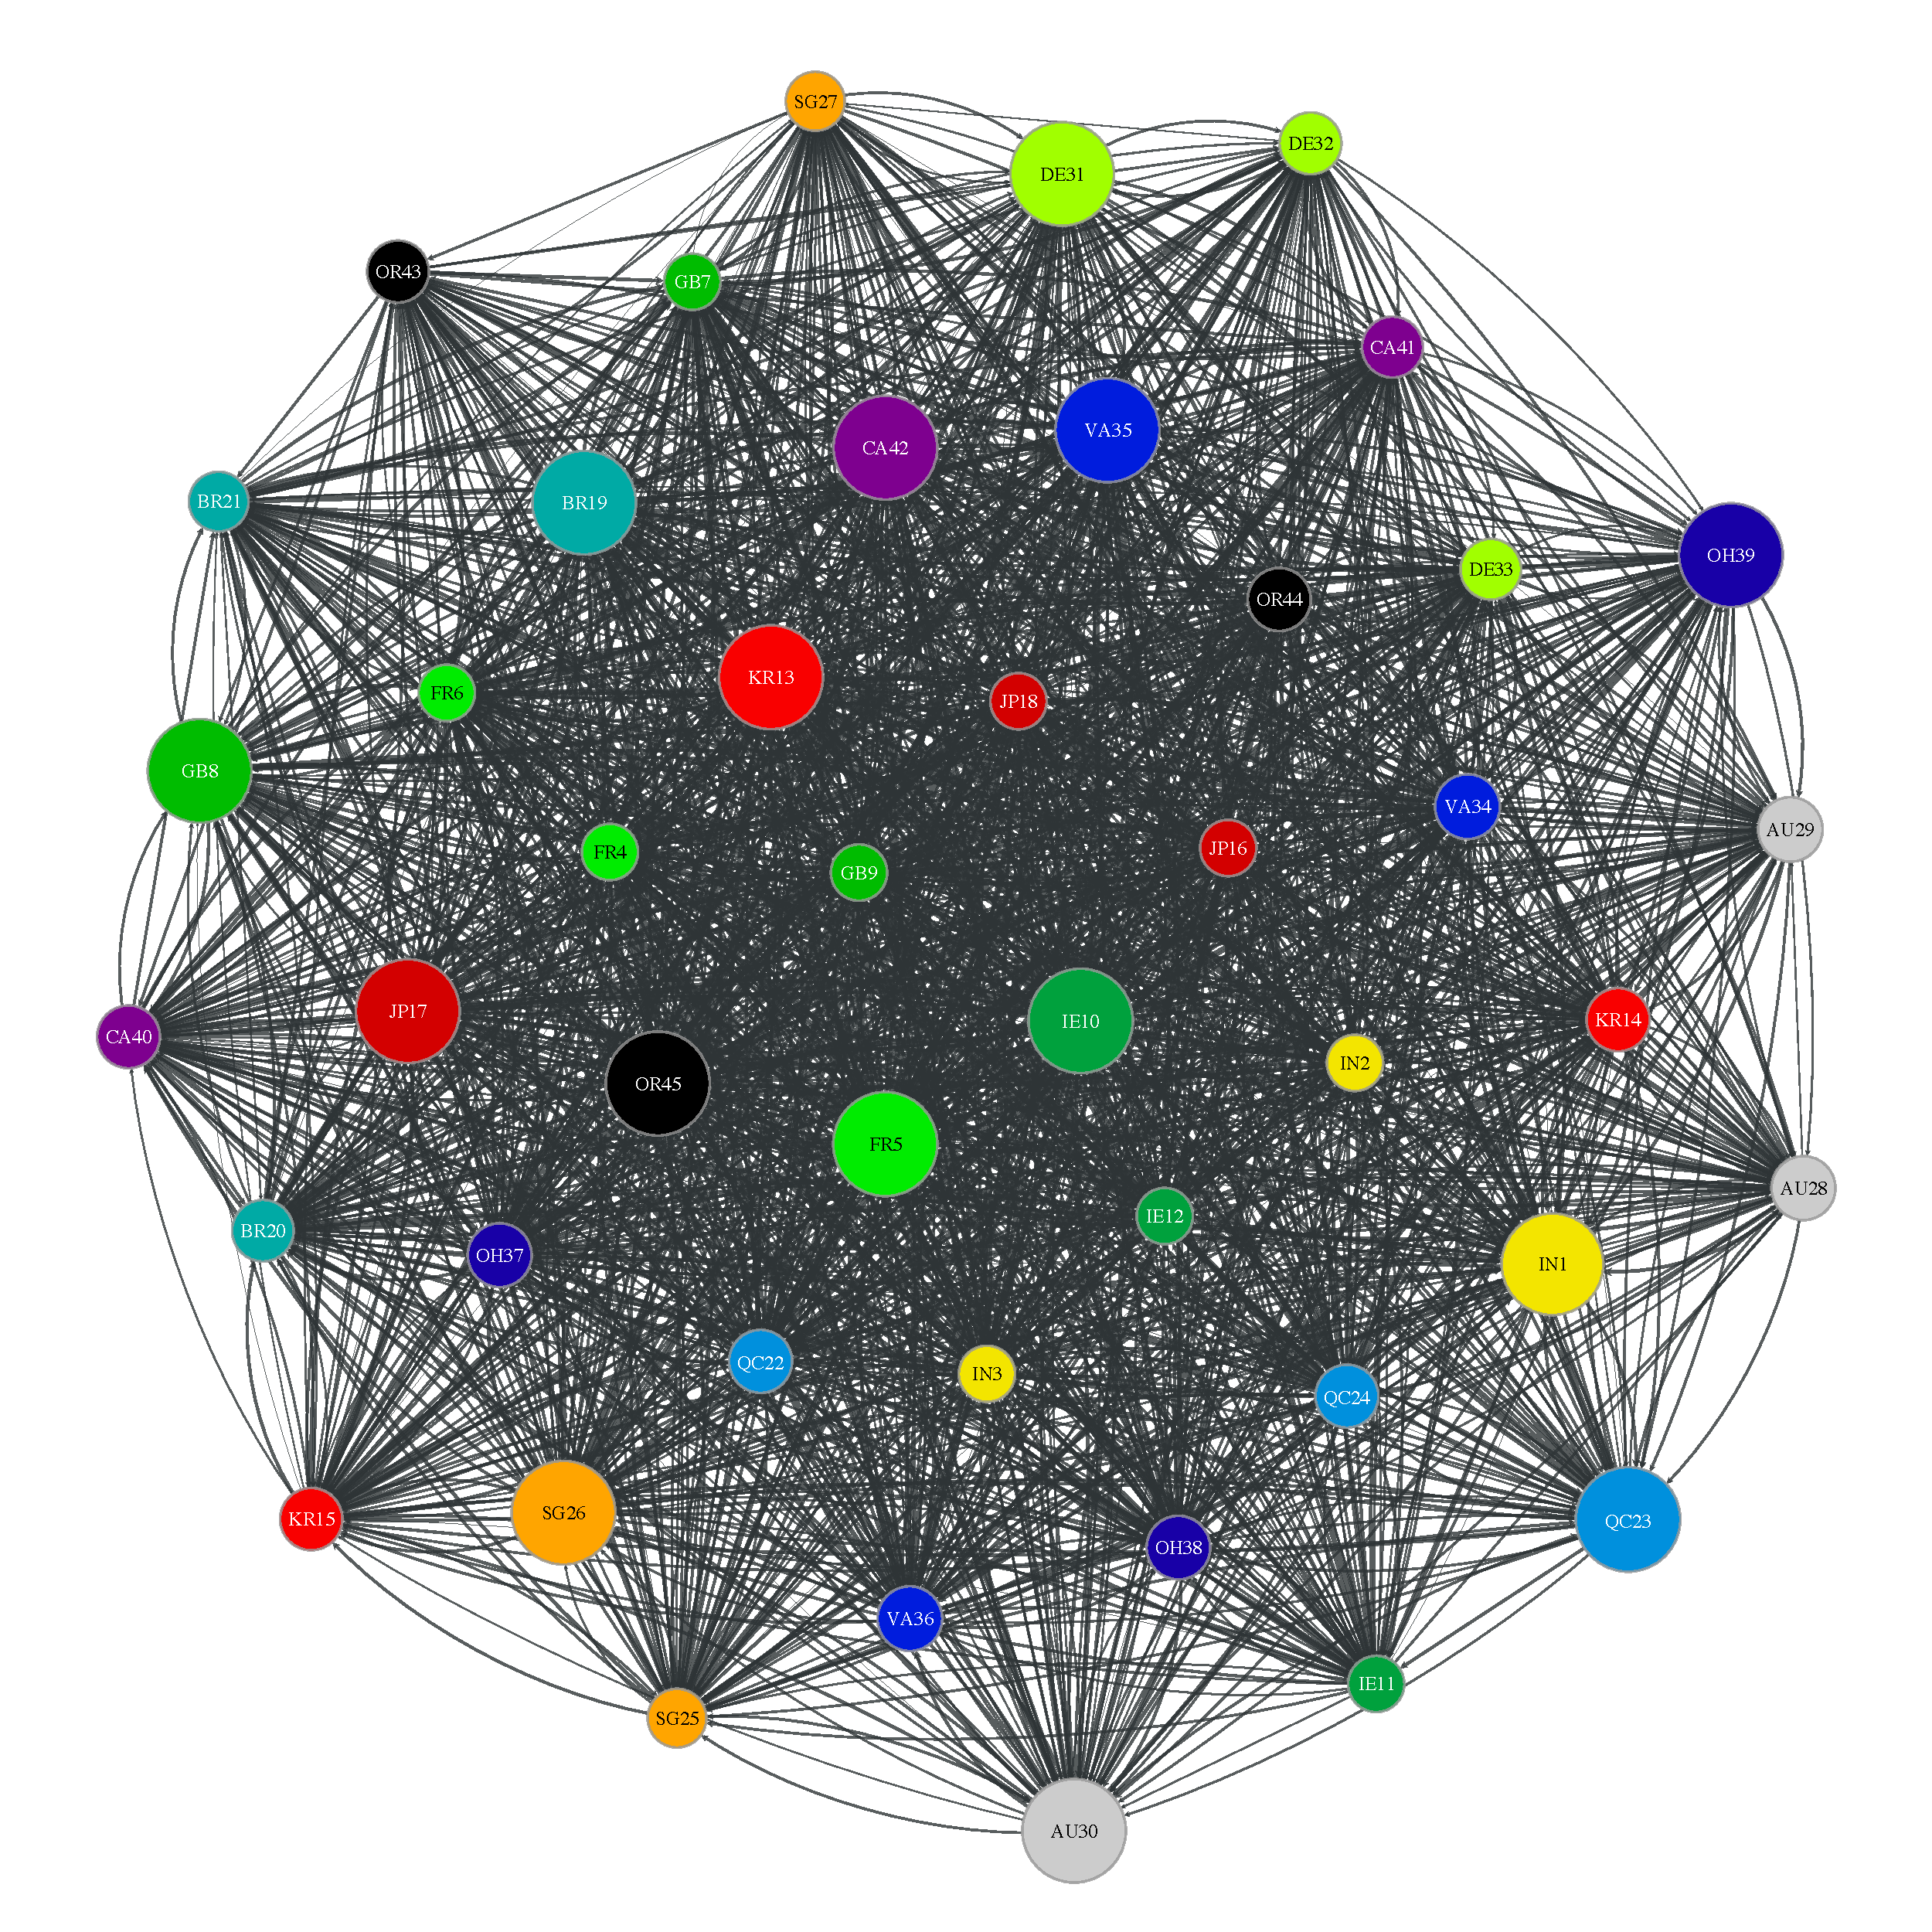
\includegraphics[width=5in]{figures/ch06_b-uniform-selection-e1.pdf}
    \end{center}
    \renewcommand{\baselinestretch}{1}
    \small\normalsize

    \begin{quote}
        \caption[Uniform Anti-Entropy Synchronization Network]{Synchronization network using uniform random selection of synchronization peers.}
        \label{fig:ch06_uniform_selection_topology}
    \end{quote}
\end{figure}
\renewcommand{\baselinestretch}{2}
\small\normalsize

\begin{figure}
    \begin{center}
        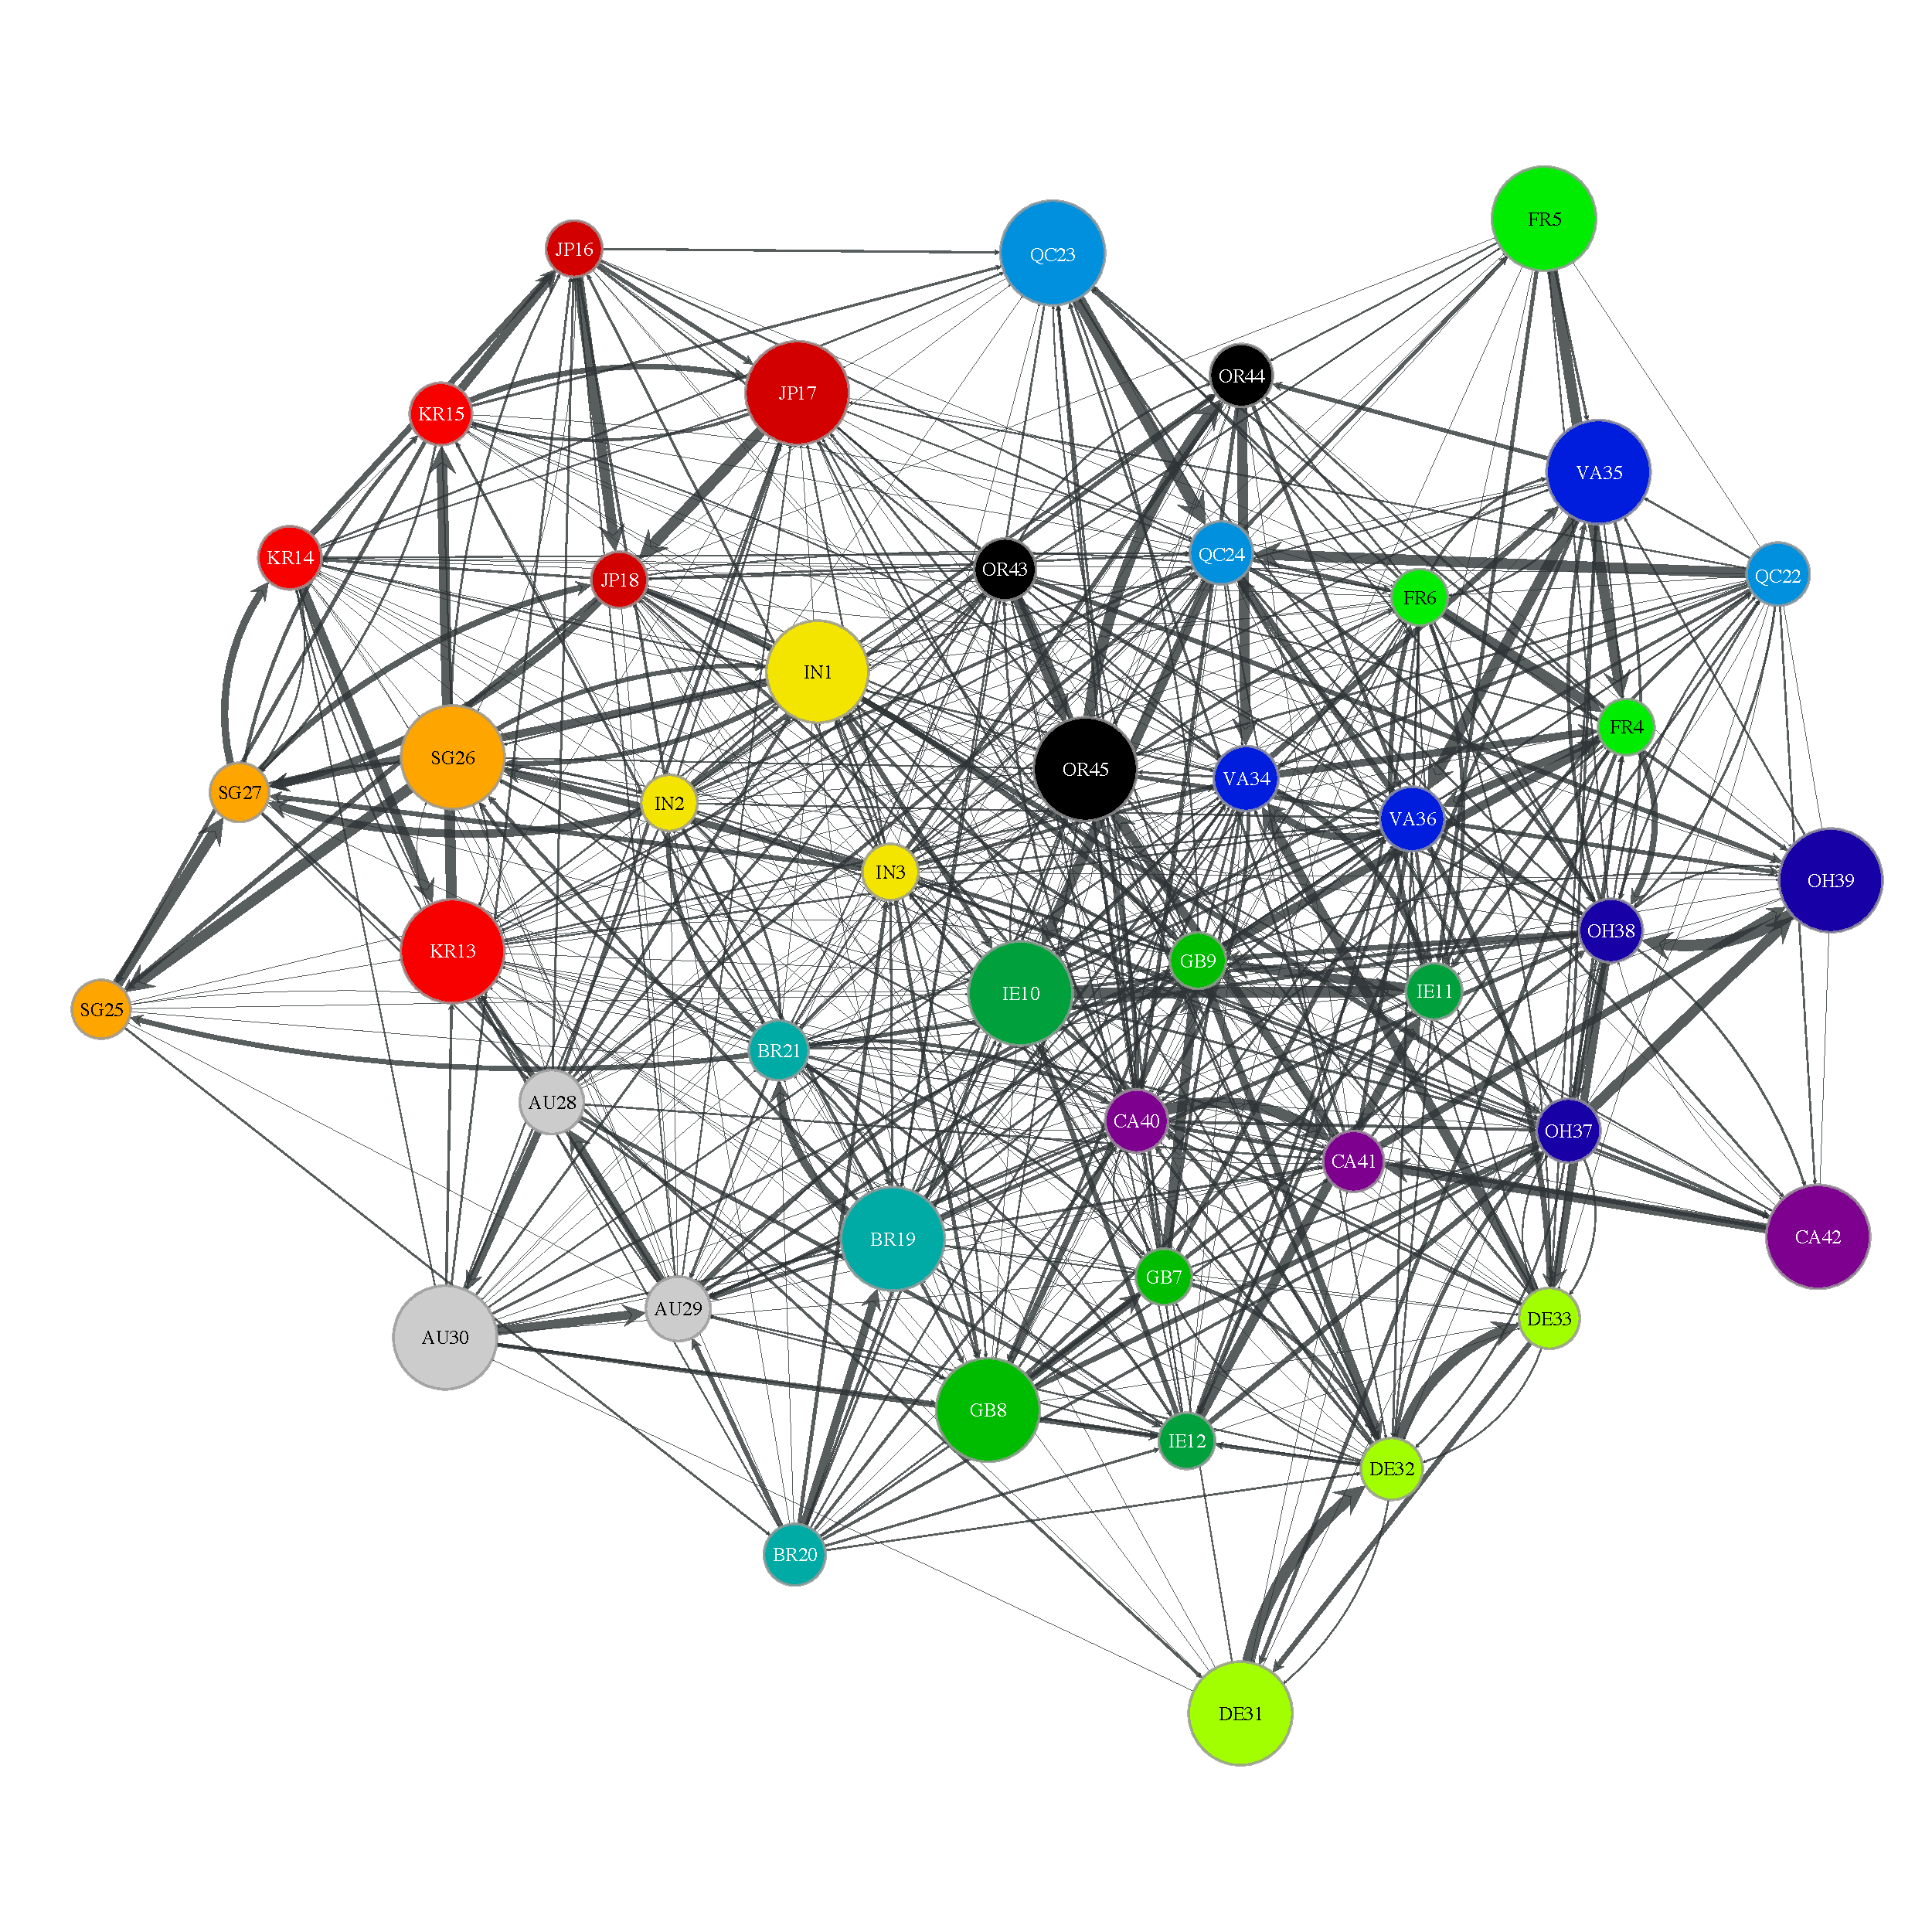
\includegraphics[width=5in]{figures/ch06_b-epsilon-greedy-0-2-e3.pdf}
    \end{center}
    \renewcommand{\baselinestretch}{1}
    \small\normalsize

    \begin{quote}
        \caption[Greedy Epsilon Anti-Entropy Synchronization Network]{Synchronization network using bandit based selection of synchronization peers with $\epsilon=0.2$.}
        \label{fig:ch06_epsilon_greedy_topology}
    \end{quote}
\end{figure}
\renewcommand{\baselinestretch}{2}
\small\normalsize

\begin{figure}
    \begin{center}
        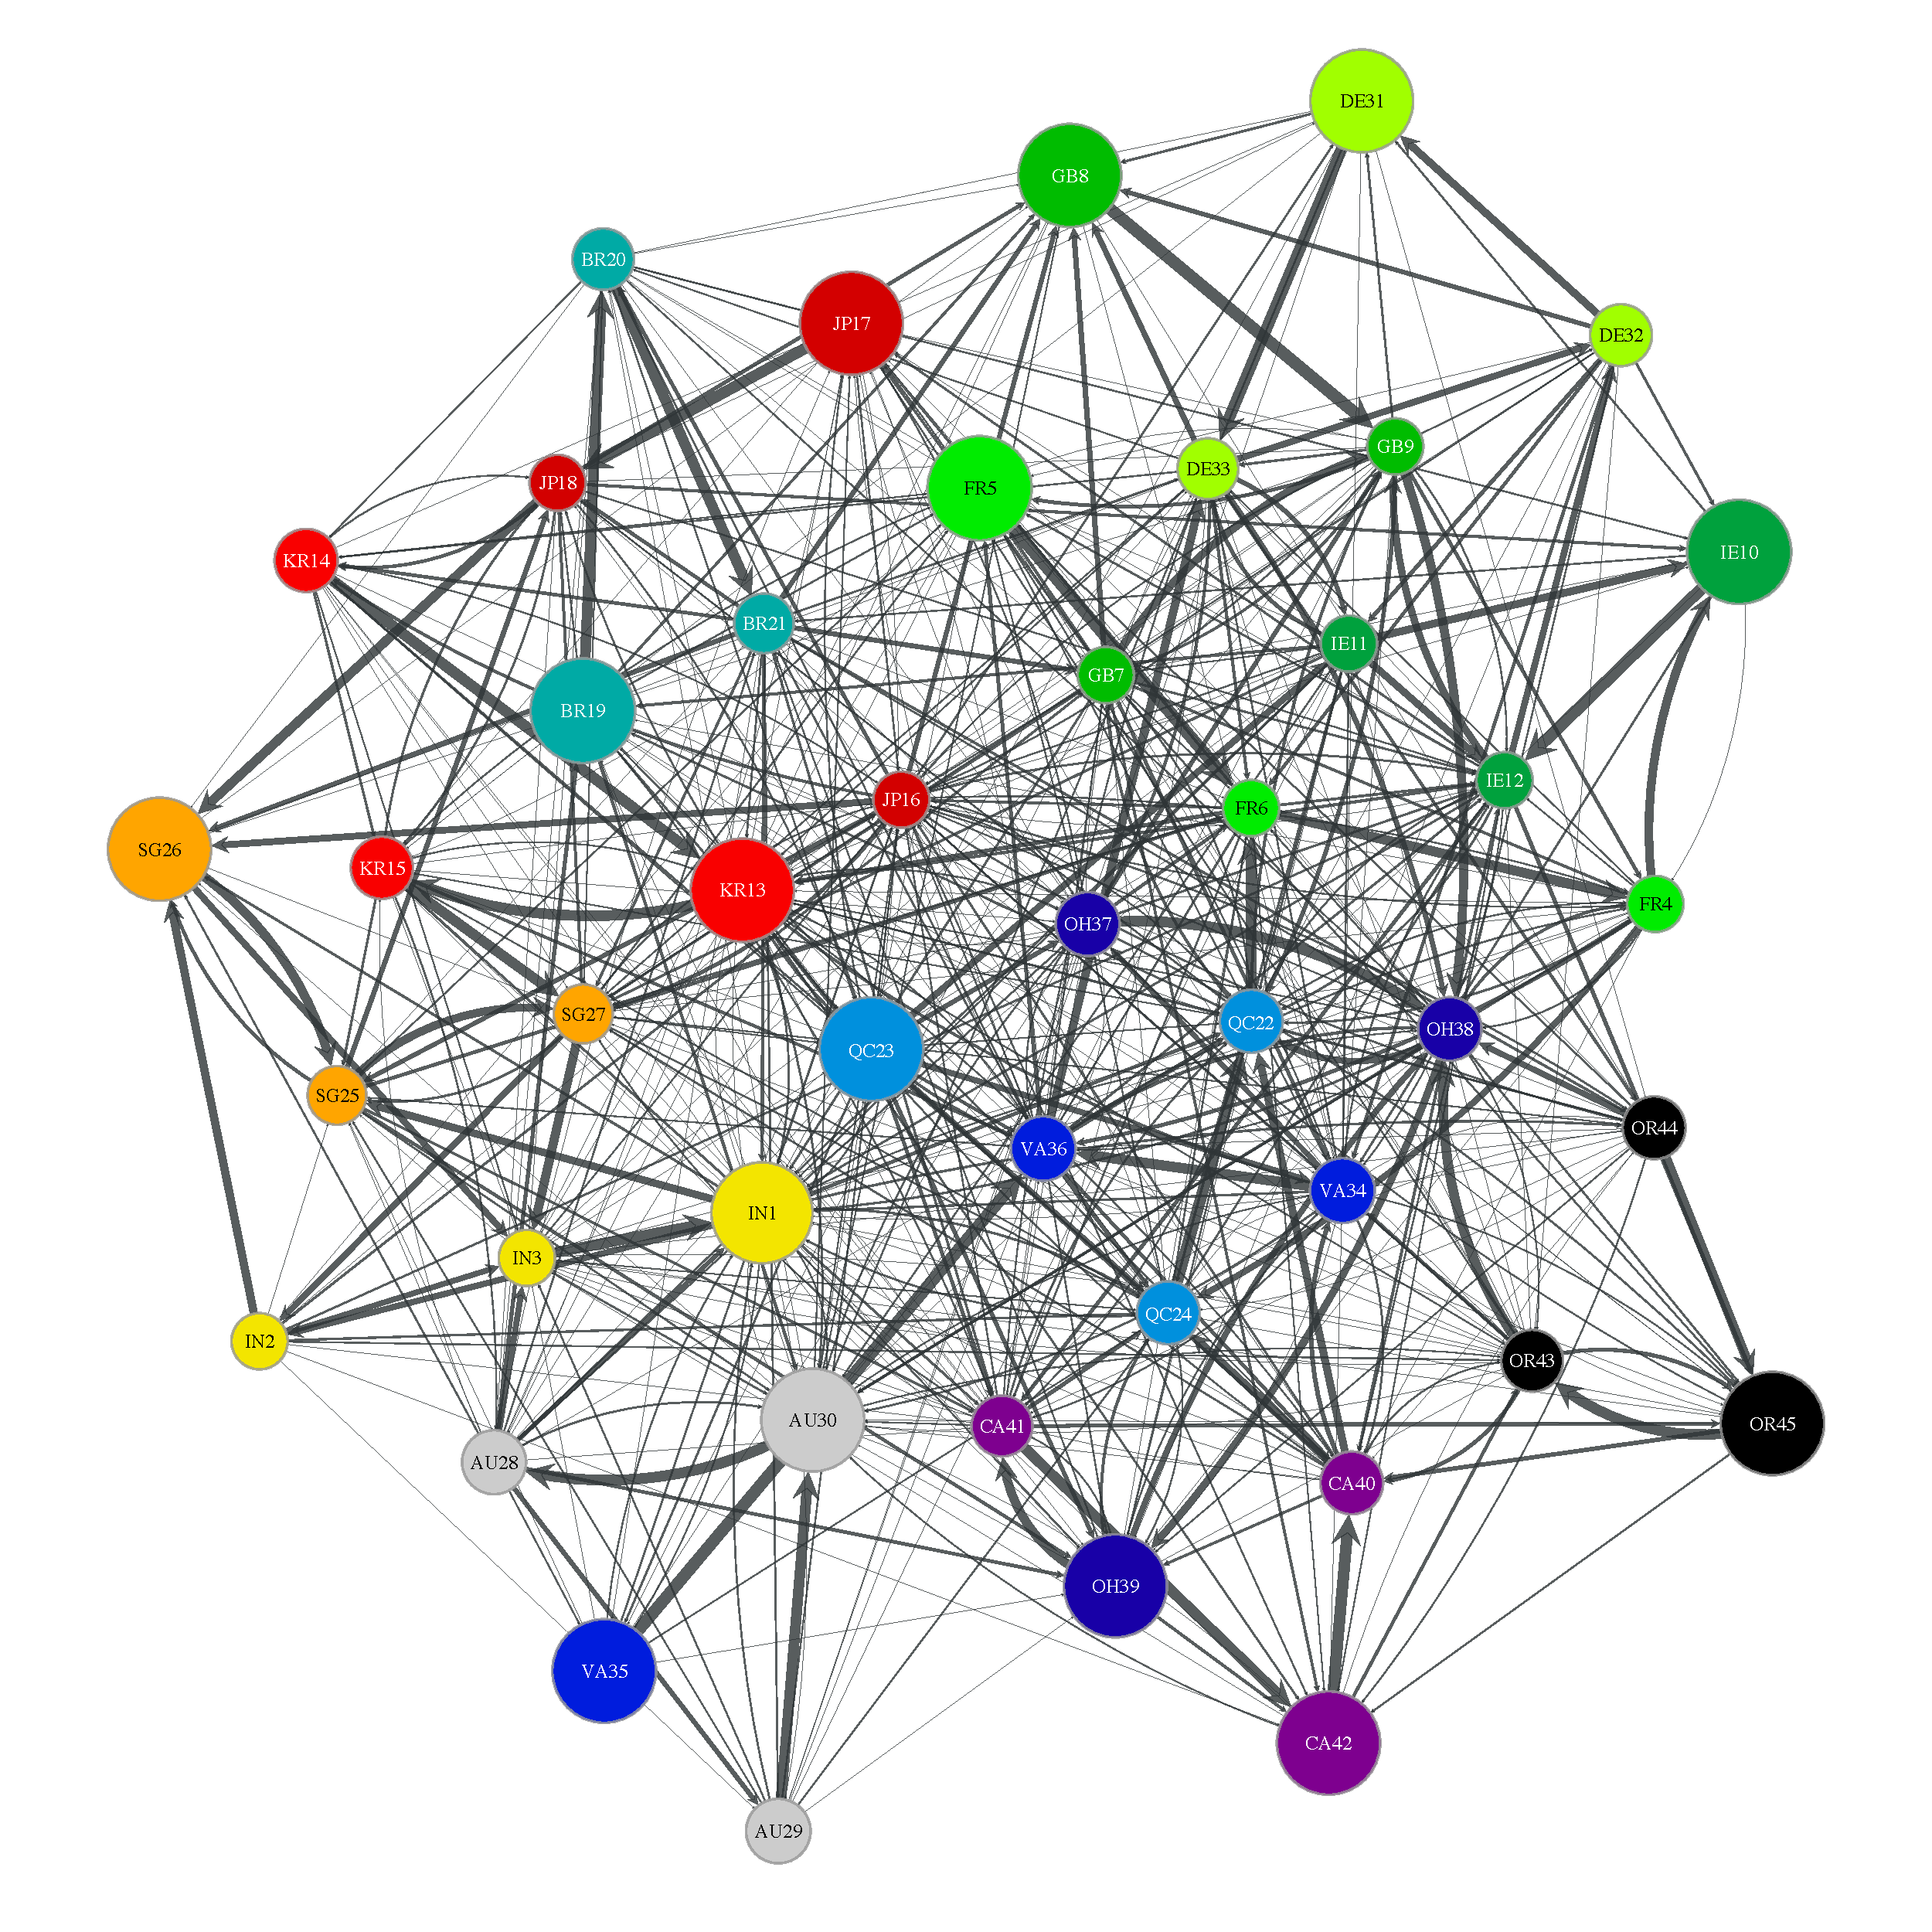
\includegraphics[width=5in]{figures/ch06_b-annealing-epsilon-greedy-e5.pdf}
    \end{center}
    \renewcommand{\baselinestretch}{1}
    \small\normalsize

    \begin{quote}
        \caption[Annealing Epsilon Anti-Entropy Synchronization Network]{Synchronization network using annealing epsilon bandit based selection of synchronization peers.}
        \label{fig:ch06_annealing_epsilon_toplogy}
    \end{quote}
\end{figure}
\renewcommand{\baselinestretch}{2}
\small\normalsize

Comparing the resulting networks, it is easy to see that more defined topologies result from the bandit-based approaches.
The uniform selection network is simply a hairball of connections with a limited number of synchronizations.
By contrast, clear optimal connections have emerged with the bandit strategies; dark lines represent extremely successful synchronization connections between replicas, while light lines represent synchronization pairs that are selected less frequently.
Based on our observations, we posit that fewer edges in the graph represents a more stable network; the fewer synchronization pairs that are selected, the less noise that occurs from selecting a peer that is in a similar state.

\section{Bandits Discussion}
\label{ch06_bandits_discussion}

To achieve stronger eventual consistency, the visibility latency
of a system replicated with anti-entropy must be reduced.
We believe that this can be achieved with two primary goals: increasing
the number of successful synchronizations and maximizing the number
of local and regional synchronizations such that the average latency of
anti-entropy sessions is as low as possible.
These goals must also be tempered against other requirements, such as
fault and partition tolerance, a deterministic anti-entropy solution that
ensures the system will become consistent eventually, and load balancing
the synchronization workload evenly across all replicas.

Bandit based approaches to peer selection clearly reduce noise inherent
in uniform random selection as shown in Figure~\ref{fig:ch06_rewards}.
The bandit strategies achieve better rewards over time because peers
are selected that are more likely to have an update to synchronize.
Moreover, based on the network diagrams shown in
Figures~\ref{fig:ch06_uniform_selection_topology}-\ref{fig:ch06_epsilon_greedy_topology}, this is
not the result of one or two replicas becoming primary syncs: most
replicas have only one or two dark in-edges meaning that most replicas
are only the most valuable peers for one or two other replicas.

Unfortunately, the rewards using a bandit approach, while clearly better
than the uniform case, are not significantly better -- this is an interesting
demonstration of the possibility of adaptive systems to improve consistency
but further investigation is required.
The primary place we see for adjustment is future work to explore the reward
function in detail.
For example, the inclusion of penalties (negative rewards) might make
the system faster to adjust to a high quality topology.
Comparing reward functions against variable workloads may also reveal a
continuum that can be tuned to the specific needs of the system.

As for localization, there does appear to be a natural inclination for
replicas that are geographically proximate to be a more likely selection.
In Figure~\ref{fig:ch06_epsilon_greedy_topology}, replicas in Canada (light blue),
Virginia (dark blue), Sydney (grey), California (purple), and Frankfurt
(light green) all prioritize local connections.
Regionally, this same figure shows strong links such as those between Ohio
and California (\texttt{CA42} $\rightarrow$ \texttt{OH38}) or Japan and
Singapore (\texttt{JP17} $\rightarrow$ \texttt{SG25}).
Replicas such as \texttt{BR19} and \texttt{IN3} appear to be hubs that
specialize in cross-region collaboration.
Unfortunately there does also seem to be an isolating effect, for example
Sydney (grey) appears to have no significant out of region synchronization
partners.
Isolated regions could probably be eliminated by scaling rewards with
the number of transmitted updates, or by using larger epsilons.
Multi-stage bandits might be used to create a tiered reward system to
specifically adjust the selection of local, regional, and global peers.
Other strategies such as upper confidence bounds, softmax, or Bayesian
selection may also create more robust localization.

Finally, and perhaps most significantly, the experiments conducted in
this paper were on a static workload; future work must explore dynamic
workloads with changing access patterns to more closely simulate real
world scenarios.
While bandit algorithms are considered online algorithms that do respond
to changing conditions, the epsilon greedy strategy can be slow to change
since it prefers to exploit high-value arms.
Contextual bandits use side information in addition to rewards to make
selection decisions, and there is current research in exploring contextual
bandits in dynamic worlds that may be applicable~\cite{contextual_bandits}.
Other strategies such as periodic reseting of the values may incur a small
cost to explore the best anti-entropy topology, but could respond to changing
access patterns or conditions in a meaningful way.

Future efforts will consider different reward functions, different selection
strategies, dynamic environments, and how the priorities of system designers
can be embedded into rewards.
Reward functions that capture more information about the expected workload of
the system such as object size, number of conflicts, or localizing objects
may allow specific tuning of the adaptive approach.
We will also specifically explore in detail the effect of dynamic workloads
on the system and how the reinforcement learning can adapt in real time to
changing conditions.
We plan to investigate periodic resets, anomaly detection, and auction
mechanisms to produce efficient topologies that are not brittle as access
patterns change.
We also plan to evaluate other reinforcement learning strategies such as
neural or Bayesian networks to determine if they handle dynamic environments
more effectively.

\section{Generalizing Adaptation}
\label{ch06_generalizing_adaptation}

% I would very much like to redo this section.

Using bandits for anti-entropy peer selection is a demonstration of an introspective model of adaptability~\cite{oceanstore}.
Introspection is an architectural paradigm that augments a systems normal operation with two components: \emph{monitoring} and \emph{optimization}.
Monitoring components must keep track of a historical record of system behavior, often summarizing or aggregating information at local nodes to minimize the amount of data that must be propagated to neighbors.
Optimization components use the observed and summarized data to extract patterns of behavior which can then be used to adapt the behavior of a system either by adjusting the configuration of a local replica~\cite{oates_investigating_1998} or by providing predictive models that are propagated to all replicas with active learning~\cite{kalai_efficient_2005,osugi_balancing_2005}.

Adaptation improves the manageability, performance, and consistency of the system in a number of ways.
Monitoring of data movement can establish continuous confidence intervals of the durability of the system and the requirements for archiving blocks in deep storage.
Adaptation can also be used to identify unreliable groups of machines or to detect anomalies that may destabilize the system.
Accesses might be classified to tune portions of the system to handle high throughput small updates vs fewer, high volume writes, or to support more reads than writes.
We believe that most systems administration tasks at a planetary scale will require some form of stochastic online adaptation behavior because a centralized monitoring and manual management is simply unrealistic.
Currently there are two primary goals for learning based adaptation that will guide the architecture for other adaptive services: object placement and replica management.

\emph{Replica management} adjusts the network topology to serve requests as efficiently as possible, repairing outages to ensure the system is maximally available.
Replicas monitor message latencies when communicating between replicas, constructing a network proximity map that influences timing parameter behavior and the system tick rate.
Message latencies can also be used to adapt other configurations in real time, such as synchronization probabilities as described by the bandit approach in this chapter or to modify the integration of federated consistency protocols.
Network proximity between replicas and clients can also be used to ensure that clients experience a high quality of service, by ensuring that quorums are constructed as close as possible to the objects the quorums serve.

Replica management can also elastically scale and provision extra capacity when needed reducing capacity when it is not.
In a planetary system, there is an expected pattern of accesses, e.g. many objects will be accessed more during daylight hours and less frequently at night.
Other objects will experience geographically shifting access patterns, for example, as passengers travel between locations on flights.
If access patterns can be extracted for specific objects or groups of objects, then optimistic root quorum decisions to allocate new quorums with hot spares or shift the locale of the quorums managing an object will increase the overall quality of service of the system.

\emph{Object placement} groups related or similar objects together to ensure inter-object consistency is maintained and to minimize access latency from a variety of geographic locations.
Hierarchical consensus is most efficient when subquorums manage accesses to a group of objects from a specific geographic locale.
If accesses to related objects cross subquorum boundaries, then remote reads between subquorums is required to maintain linearizable consistency.
Automatic discovery of relationships between objects ensures that a single subquorum manages the objects most likely to be accessed together thereby minimizing the access latency.
Alternatively if reads and writes of an object are from different regions, the frequency of the type of access in each region can determine how to configure a subquorum for maximum benefit.
Clustering algorithms can also be used to group objects and to prefetch them to locales of expected access.

The challenge for generalized adaptation is to carefully balance local behaviors and coordinated learning.
In principle, local reinforcement learning is preferred so that neighborhoods of common behavior emerge, creating efficient global behaviors.
However, other learning techniques such as anomaly detection, event classification, or confidence reporting require a global view of access patterns and the network environment.
Balancing these two opposing requirements is an area of essential future research, though one that requires real data to demonstrate the influence of learning systems on consistency.

\section{Conclusion}

In this chapter we have presented a demonstration of adaptive consistency in
the geo-replicated eventually consistent systems by employing a novel
approach to peer selection during anti-entropy -- replacing uniform random
selection with multi-armed bandits.
Multi-armed bandits consider the historical reward obtained from
synchronization with a peer, defined by the number of objects synchronized
and the latency of RPCs, when making a selection.
Bandits balance the exploitation of a known high-value synchronization
peer with the exploration of possibly better peers or the impact of
failures or partitions.
The end result is a replication network that is less perturbed by noise
due to randomness and capable of more efficiently propagating updates.

In an eventually consistent system, efficient propagation of updates is
directly tied to higher consistency.
By reducing visibility latency, the likelihood of a stale read decreases,
which is the primary source of inconsistency in a highly available system.
We have demonstrated that bandit approaches do in fact lower visibility
latency in a large network.

We believe that the results presented show a promising start to a renewed
investigation of highly available distributed storage systems in novel
network environments, particularly those that span the globe.
Specifically, this work is part of a larger exploration of adaptive,
globally distributed data systems that federate consistency levels to provide
stronger guarantees~\cite{federated_consistency_poster}.
Federated consistency combines adaptive eventually consistent systems such as
the one presented in this paper with scaling geo-replicated consensus such as
Hierarchical Consensus~\cite{hc_brief_announcement} in order to create robust
data systems that are automatically tuned to provide the best availability
and consistency.
Distributed systems that adapt to and learn from their environments and
access patterns, such as the emerging synchronization topologies we observed
in this paper, may form the foundation for the extremely large, extremely
efficient networks of the future.

%Chapter 7

\renewcommand{\thechapter}{7}

\chapter{Related Work}
\label{ch:related_work}

Spanner~\cite{spanner} provides global consistency by sharding each tablet across multiple Paxos groups then externalizes their consistency using TrueTime, delaying the commit until a window of uncertainty has passed.

CalvinFS~\cite{calvindb,calvinfs} batches transaction operations across the wide area, but still requires paxos to be deployed across the wide area.

Systems that implement many small quorums of
coordination~\cite{mdcc,scatter,spanner} avoid the centralization bottleneck
and reliability concerns of master-service
systems~\cite{gray_dangers_1996,gfs} but create silos of independent
operation that are not coordinated with respect to each other.

We have theorized that cloud services present the opportunity for deploying data services on a trusted infrastructure. If it is not trusted, however, we can use an encryption model similar to SPORC to combine multiple cloud providers into a single data system~\cite{sporc}. 

\section{Hierarchical Consensus}

Our principle contribution is Hierarchical Consensus, a general technique to compose consensus groups, maintain consistency invariants over large systems, and adapt to changing conditions and application loads.
HC is related to the large body of work improving throughput in distributed consensus over the Paxos protocol~\cite{paxos,epaxos,fexible_paxos,generalized_paxos}, and on Raft~\cite{raft,raft_refloated}.
These approaches focus on fast vs. slow path consensus, eliding phases with dependency resolution, and load balancing.

Our work is also orthogonal in that subquorums and the root quorums can be implemented with different underlying protocols, though the two levels must be integrated quite tightly.
Further, HC abstracts reconfiguration away from subquorum consensus, allowing multiple subquorums to move into new configurations and reducing the need for joint consensus~\cite{raft} and other heavyweight procedures.
Finally, its hierarchical nature allows the system to multiplex multiple consensus instances on disjoint partitions of the object space while still maintaining global consistency guarantees.

The global consistency guarantees of HC are in direct contrast to other systems that scale by exploiting multiple consensus instances~\cite{bigtable,mdcc,spanner} on a per-object basis.
These systems retain the advantage of small quorum sizes but cannot provide system-wide consistency invariants.
Another set of systems uses quorum-based decision-making but relaxes consistency guarantees~\cite{dynamo,pnuts,cops}; others provide no way to pivot the entire system to a new configuration~\cite{scatter}.
Chain replication~\cite{van2004chain} and Vertical Paxos~\cite{vertical_paxos} are among approaches that control Paxos instances through other consensus decisions.
However, HC differs in the deep integration of the two different levels.
Whereas these approaches are top down, HC consensus decisions at the root level replace system configuration at the subquorum level, and vice versa.

Possibly the closest system to HC is Scatter~\cite{scatter}, which uses an overlay to organize consistent groups into a ring.
Neighbors can join, split, and talk amongst themselves. The bottom-up approach potentially allows scaling to many subquorums, but the lack of central control makes it hard to implement global re-maps beyond the reach of local neighbors.
HC ties the root quorum and subquorums tightly together, allowing root quorum decisions to completely reconfigure the running system on the fly either on demand or by detecting changes in network conditions.

We claim very strong consistency across a large distributed system, similar to Spanner~\cite{spanner}.
Spanner provides linearizable  transactions through use of special hardware and environments, which are used to tightly synchronize clocks in the distributed setting.
Spanner therefore relies on a very specific, curated environment. HC targets a wider range of systems that require cost effective scaling in the data center to rich dynamic environments with heterogeneity on all levels.

Finally, shared logs have proven useful in a number of settings from fault tolerance to correctness guarantees.
However, keeping such logs consistent in even a single consensus instance has proven difficult~\cite{chubby,gfs,zookeeper}.
More recent systems are leveraging hardware support to provide fast access to shared logs~\cite{vcorfu,tango,calvindb,calvinfs,hyder-a,fawn}.
To our knowledge, HC is the first work to propose synchronizing shared logs across multiple discrete consensus instances in the wide area.

%Chapter 8

\renewcommand{\thechapter}{8}

\chapter{Conclusion}
\label{ch:conclusion}

Inspired by the work of Oceanstore and recent trends in cloud computing we present a consistency-centric architecture for a planetary scale data storage system.
This architecture provides support for extremely large systems with thousands or even millions of replicas geo-replicated across continents and oceans.
We envision that such a system will reside in heterogenous network environments, therefore we propose a two tier consistency model -- a hierarchical consensus core residing in cloud data centers federated with a highly available fog of devices that rapidly disseminate updates.
We also recognize that management of such a large system cannot easily be centralized therefore we also propose an adaptive scheme such that local optimizations lead to emergent global consistency.

Our work is motivated by recent trends in global scale software.
The success of cloud computing and app stores allows software developers to easily deploy their applications to an international audience.
Software development practices have shifted to meet these trends, from container based development to Web application localization, and most software is now deployed expecting international scaling.
The problem is that the data storage that backs these applications has not kept up.
International deployment therefore requires developers to isolate data in specific regions, or to use provisioned data services for geo-replicated databases developed by the cloud providers themselves.
There is a growing need for region-agnostic, generalized geo-replicated data services that provide SQL-like strong consistency guarantees.

Hierarchical consensus provides high-throughput, geo-replicated consensus to serve as a strata for the strongest possible consistency databases and file systems.
An implementation and extension of Vertical Paxos, HC shards accesses to independent subquorums, which themselves are configured by a root quorum.
The root quorum is composed by all replicas in the system to ensure maximal fault tolerance and an intersection between configuration decisions and access decisions.
To support such a large quorum, followers in subquorums delegate their votes to their leaders, who are the only active participants in the root quorum.
The root quorum makes configuration decisions to partition the object space to partitioned to subquorums localized in the region where accesses occur.
Subquorums fuzzily transition between configuration changes to ensure the system makes global progress, then replicate accesses from clients.
These techniques ensure that HC provides unified globally distributed consensus and that strong consistency semantics can be guaranteed and easily reasoned upon without region-specific considerations.

Next generation distributed systems will also have to support high throughput machine-to-machine geographically localized accesses.
Sensors systems from traffic coordination devices to the smart grid and an Internet of Things will push time-sensitive data from multiple distributed publishers, to fewer centralized subscribers.
These devices will exist in highly variable mobile network environments in a much wider area, creating a fog of extra datacenter devices that require higher availability rather than the strongest possible consistency.

We believe a single architecture should support both the cloud and the fog.
We therefore propose the consistency-centric federation of multiple synchronization protocols.
Federation of strong consistency provided by consensus and eventual consistency provided by anti-entropy synchronization involves both communication and consistency integration at the boundary of each system type.
Communication integration requires that all replicas respond to distinct RPC requests from either type of system in a manner that is correct if the system was homogenous.
Consistency integration requires the ability to communicate the strongest possible consistency back to the relaxed consistency model and resolve policy differences.
By defining a ``forte'' component of comparable version numbers, consensus leaders can arbitrate which version should be accepted across the entire system.
Federation provides a hybrid consistency model that is more continuous than discrete, depending on topology, e.g. more eventual replicas lead to higher system availability, more consensus replicas lead to higher system consistency.

Both federation and hierarchical consensus allow systems to scale to thousands of replicas and millions of clients.
At this scale, centralized system management and configuration tuning becomes intractable.
Our final proposition is for adaptive consistency -- the use of real-time machine learning to adjust the configuration of the system to maximize the consistency guarantees of the system.
Adaptive consistency monitors network behavior, access patterns, and object attributes locally, modifying the behavior of individual replicas.
This information is then forwarded to optimization computations that create global models which are disseminated to target replicas for decision making or to reconfigure replica or object placement.

We demonstrated the potential for adaptive consistency with a reinforcement learning approach to peer selection for anti-entropy.
Using multi-armed bandits, replicas modified the likelihood of selecting a peer for synchronization based on observing how successful the synchronization was.
By rewarding low latency connections as well as multiple objects sync'd, the network as a whole learned a topology based on accesses that efficiently propagated updates across the system.
This in turn reduced the visibility latency of a write, and reduced visibility latency means a lower probability of stale reads, the root cause of inconsistency.
Therefore anti-entropy bandits increased the overall consistency of the system.
We propose that replicas learning locally and creating emergent global properties is the best strategy for decentralized adaptation of the system.

Together, our observations about strong geo-distributed consensus, federated consistency, and adaptive consistency form a complete model for planetary scale systems.
Our architecture is composed of an HC core that propagates updates through broadcast mechanisms across the wide area while federating an eventual system in the fog, all of which is managed by adaptive consistency.
We evaluated HC with a system implementation spanning the globe, focused on maximizing throughput and minimizing access latency.
We evaluated our federated consistency model with a simulation to collect metrics that are difficult to measure in a distributed system.
Finally, we experimented with adaptive consistency using our eventual system, also distributed around the globe, optimizing the network based on global accesses.
We believe these systems create a rich platform for a variety of future lines of inquiry and research.

To date we have implemented the HC (Alia) and Fog (Honu) components individually.
Our next step is to federate them into a single system, moving our simulation experiments into the real world.
Both HC and Fog currently implement a distributed key/value store.
Our target application is a globally distributed file system, which will serve as a replication substrate for other applications.
Our file system, FluidFS, is currently implemented using a key/value store replicated using standard consensus algorithms.
By replacing consensus with our planetary scale consistency system, we believe that FluidFS will be able to support truly massive applications.

Once we have our fully integrated system, we plan to deploy it as two primary applications.
The first application is a direct deployment of FluidFS as a shared cloud storage drive.
The second application we envision is a global trading-card game.
In this game, users will use matchmaking to find other players to play 2--4 person short games and will be able to trade cards.
In particular we envision a system such that each region has its own faction with its own abilities to foster trading across the wide area.
Although the details are beyond the scope of this dissertation, these applications are designed to exercise the planetary scale system in meaningful ways.

We believe that the open source nature of our project will foster adoption and interest in these applications.
Even if the applications are short lived, real world workloads and access traces will allow us to create planetary-scale benchmarks that simply do not exist right now.
Additionally, real world deployments will allow us to construct realistic models of outages and downtime that will more easily allow us to test future research.
Finally, most of the questions around adaptive consistency require non-synthetic data to construct and evaluate models.
Acquiring real world users will allow us to address many future questions.

The most pressing question concerns when to make HC root decisions.
Currently, reconfiguration is manually triggered or triggered by simple heuristics appropriate to the experiments we were running.
However, new epochs should be proposed by monitoring demand and access patterns, ensuring that subquorums are localized with respect to their accesses.
The root quorum must monitor replica health and object placement to create a measurement of the ``system quality,'' then if a threshold in the quality metric is reached, it should adapt the system to improve or optimize quality.
Adaptive consistency and learning methods might also be used to pre-allocate subquorums to ensure there is as little down time as possible.

Our next question concerns the implementation of transactions in HC.
Our current implement does not directly implement transactions but does allow client-side transactions by allowing remote reads and writes to coordinate multi-object accesses.
Native support for transactions would significantly increase geo-replicated consistency, however, particularly if the native support fit into the hierarchical model.
We propose to investigate a transaction tier or other structural patterns such as batching transactions across the wide area in a hierarchical context.

We would like to explore adaptations of other consensus protocols.
We described HC with leader-oriented consensus, primarily because it allowed us to more easily reason about delegation.
We see no reason that leaderless consensus such as ePaxos or leader balanced mechanisms like Mencius could not fit into hierarchical consensus.
For example, if accesses are evenly balanced around a region of interest; for example between Ireland, London, and Frankfurt -- then an ePaxos subquorum would perform far better than a Raft subquorum.
The second generation of hierarchical consensus will support multiple consensus protocols that are designed to optimize subquorum behavior, configured by the root leader.

A weak point of HC is the obligations timeout that occurs when a single subquorum is partitioned from the rest of the system.
We briefly mentioned that federated consistency might provide flexibility to solve this issue by allowing the subquorum to relax consistency for the duration of the partition.
We would like to explore this in detail, particularly as the focus of our federated work was on how to make an eventual consistency system stronger with a core consensus background.
Federation creates a data fabric, where updates can be propagated across multiple channels, which we believe leads to important research questions about how such a mesh would influence failure behavior.

Another line of inquiry is the ability to federate other consistency protocols and automatically handle conflicts.
Causal consistency is ``the strongest form of weak consistency'' and we see no reason why it cannot be federated using similar strategies to the ones we proposed.
Any time consistency is relaxed, the possibility of conflicts increases.
However, users do not necessarily have to resolve conflicts just because a collision occurs.
Causal relations and dynamic blocking such as the ones used in Git may allow the system to automatically resolve conflicts.
We believe that enhancing conflict resolution as a native part of federated consistency will create much more robust policies than latest-writer-wins, which will lead to more robust generalized federation.

Using machine learning to automatically adapt and tune system behavior is also a large and important area of interest.
These techniques will play a large role in automatically scaling the system to meet demand at peak periods and to rollback resources to conserve energy.
Clustering objects and other smart access techniques will allow not only for faster cache access but also improve consistency overall.
We expect that systems research will natively move to including learning systems in the same way that security is taken seriously in systems now.

The object of this work was to consider a consistency-centric planetary scale data model.
This model will serve as a platform for future research into geo-replicated consensus and consistency.
As geographically distributed systems become more essential to software development, we hope that the open source nature of our software and the investigation proposed in the dissertation serve as a basis and inspiration
to bring the benefits of technology to every part of the earth, and perhaps farther.

% \titleformat{\chapter}
% {\normalfont\large}{Appendix \thechapter:}{1em}{}
% \appendix
\renewcommand{\thechapter}{A}
\renewcommand{\chaptername}{Appendix}

\chapter{Formal Specification}

Will add formal specification here.

% %Appendix -- January 2015
\appendix
\renewcommand{\thechapter}{B}
\renewcommand{\chaptername}{Appendix}

\chapter{Other Resources and Texts}


\renewcommand{\baselinestretch}{1}
\small\normalsize
% \begin{thebibliography}{99}
\setlength{\parskip}{1em}

\end{thebibliography}
 %Delete this line if using Bibtex or Natbib

%When using Bibtex, delete the previous line and use the following
%three lines:
\newpage
\bibliographystyle{unsrt}
\bibliography{Bibliography}

%When using Natbib, use the following three lines:
%\newpage
%\bibliographystyle{unsrtnat}
%bibliography{Galactic,Dottie} %replace "Galactic,Dottie" with the
%                 file name(s) of your bib file(s)

\end{document}
